% multiple1902 <multiple1902@gmail.com>
% doctor.tex
% Copyright 2011~2012, multiple1902 (Weisi Dai)
% https://code.google.com/p/xjtuthesis/
% 
% It is strongly recommended that you read documentations located at
%   http://code.google.com/p/xjtuthesis/wiki/Landing?tm=6
% in advance of your compilation if you have not read them before.
%
% This work may be distributed and/or modified under the
% conditions of the LaTeX Project Public License, either version 1.3
% of this license or (at your option) any later version.
% The latest version of this license is in
%   http://www.latex-project.org/lppl.txt
% and version 1.3 or later is part of all distributions of LaTeX
% version 2005/12/01 or later.
%
% This work has the LPPL maintenance status `maintained'.
% 
% The Current Maintainer of this work is Weisi Dai.
%
\documentclass[
    doctor,
    truefont,
    %nofont, % remember to manally set the fonts
    pdflinks,
    %colorlinks,
    %compact,
    ]{xjtuthesis}

\usepackage[vlined,ruled,linesnumbered]{algorithm2e}    
\usepackage{booktabs}
\renewcommand{\eqref}[1]{公式(\ref{#1})}
\newcommand{\figref}[1]{图~\ref{#1}~}
\renewcommand{\algorithmcfname}{\bf ~算法~ }


\ifnum 4>3
%明审
\def\authornames{\BlindPeerReviewOFF}
\def\swithON{\BlindPeerReviewOFF}
\else
%盲审
\def\authornames{\BlindPeerReview}
\def\swithON{\BlindPeerReviewON}
\fi
\graphicspath{{figures/}}

\begin{document}

% multiple1902 <multiple1902@gmail.com>
% meta.tex
% Copyright 2011~2012, multiple1902 (Weisi Dai)
% https://code.google.com/p/xjtuthesis/
% 
% It is strongly recommended that you read documentations located at
%   http://code.google.com/p/xjtuthesis/wiki/Landing?tm=6
% in advance of your compilation if you have not read them before.
%
% This work may be distributed and/or modified under the
% conditions of the LaTeX Project Public License, either version 1.3
% of this license or (at your option) any later version.
% The latest version of this license is in
%   http://www.latex-project.org/lppl.txt
% and version 1.3 or later is part of all distributions of LaTeX
% version 2005/12/01 or later.
%
% This work has the LPPL maintenance status `maintained'.
% 
% The Current Maintainer of this work is Weisi Dai.
%

\ctitle{ 面向网络MAC层的无线资源管理与控制关键技术研究}

\ifx\authornames\swithON
%明审
    \cauthor{燕志伟}
    \csupervisor{刘贵忠~ 教授}
    \eauthor{Zhiwei Yan}
    \esupervisor{Prof. Guizhong Lui}
\else
%盲审
    \cauthor{ }
    \csupervisor{}
    \eauthor{ }
    \esupervisor{}
\fi


\csubject{信息与通信工程}
\ckeywords{无线资源管理; MAC层; 基站切换; 呼叫接入控制; 博弈论}
\cproddate{\the\year 年\the\month 月}
\ctype{应用基础}

\etitle{Radio Resource Management and Control on MAC Layer}
\ekeywords{Radio resource management; MAC; Handover; Call admission control; Game theory}
\ecate{Philosophy}
\esubject{Information and Communication Engineering}
\eproddate{\monthname{\month}\ \the\year}
\etype{Application Fundamentals}

\cabstract{
信息技术与互联网的迅猛发展,极大地推动了人们对无线互联网及移动互联网应用的需求。新的互联网应用的出现,例如Facebook、Twitter等,也使人们对网络的依赖性逐步增强。
与此同时,宽带网络以及无线网络日新月异的技术发展,使人们感受到了宽带无线网络给人们生活带来的便利。
然而,无线频谱资源的稀缺性与多媒体业务日益增多的需求之间的矛盾,
却对无线资源管理的研究提出了更多的挑战。

本文从理论与应用相结合的角度出发,以无线网络的数据链路层为研究背景,
对数据链路层的资源管理与控制中的关键技术进行了深入细致地研究,取得了以下主要的研究成果。

\begin{enumerate}[(1)]
\item 
通过分析多媒体中的各种不同业务的特征,
建立了一个针对网络底层资源分配参数与网络高层业务服务质量(QoS)参数之间关系的映射模型,
实现不同业务用户的QoS水平统一标定以及系统整体性能的有效测量。
然后,基于这个映射模型,提出了一个基于系统效用和用户自身效用兼顾的呼叫接纳控制与资源分配的算法,满足不同业务QoS要求及实现系统资源的在线管理。
该算法以用户服务质量效用为最大化目标,在高负荷下依据用户业务负载情况调整接纳与资源分配策略,可以有效地提高资源利用率和保证用户的QoS水平。

\item 
针对用户资源竞争与分配的问题,提出了一个新的资源分配议价博弈模型及相应的分配算法。
从理论上分析了所提出的议价模型合理性,以及其可以满足纳什议价所提出的公理约束。
通过对议价能力的分析与讨论,提出了基于用户应用特征参数值的用户议价能力的函数定义形式。
实验的结果表明,所提出的议价博弈模型可以有效地描述用户之间的资源争用问题。
所提出的资源分配算法在保证系统资源利用率的同时,又可以兼顾单个用户自身通信资源的合理需求。

\item 
针对网络中业务逐渐增多的趋势,提出了通过连续概率随机变量来描述用户的业务类型的新方法。
与传统的离散分类方法不同,新方法可连续细致地刻化用户业务特征。
并且,根据业务随机分布情况,提出在网络不完备信息的情况下,通过构造Bayesian博弈模型的方法来寻求使用户满意的资源分配策略。
理论分析与仿真实验证明,所提出的业务描述方法、博弈模型和算法,可以有效地解决在不完备信息下的多用户竞争与资源分配问题。

\item 
针对高速移动终端的基站切换问题,通过分析移动终端的移动速度对误比特率的影响,
以及移动速度与相邻基站交叠区域距离的关系,
建立了以基于移动速度的基站切换成功概率模型。
此概率模型有效地描述了移动速度在频谱偏移和时间延迟上对切换协议信令接收与发送的影响,并直接建立了切换成功概率与移动速度之间的关系。
然后,基于此模型,提出了一个移动速度自适应的FEC保护方案。仿真结果表明,基站的切换成功率与切换效率可以有效地得到改善和提高。
\end{enumerate}
}
\endinput


\eabstract{
With the development of the Internet in recent years, 
popular demand is to keep their links to the Internet anytime and anywhere. The new Internet applications such as Facebook, Twitter, attract the people attention in their normal life.
People are experiencing the changes of their lives influenced by new technologies about broadband network and wireless networks.
However, the scarcity of radio-spectrum resource does challenge the demand of the increasing multiple media traffic from users. 
Therefore, it also challenges the intelligence of researchers for radio resource management.

This dissertation focuses on the resource management in data link layer over wireless networks, especially for the three important problems: 
handover algorithm with high velocity mobile station,  the mechanism of resource allocation in call admission control, and the application of game theory for the resource allocation.
The main work in this dissertation includes the several parts in the following:
\begin{enumerate}[(1)]

    \item According to the characteristic of multimedia traffic, the mapping model is proposed to examine the relationship between the resource management configuration in the data link layer and the quality of service in the application layer, perceived by  users. And we develop a new call admission control algorithm with the proposed mapping model. The new algorithm can manage both ongoing connections or calls and new ones efficiently. It also balances the utility of individual users and the utility of a system, especially under heavy load traffic.  

    \item In order to deal with the competition of resource among selfish users over wireless networks, we proposed a new competing model of game theory and its resource allocation algorithm. The game model introduces the Nash bargaining solution to solve the problem of competition. The proposed definition of utility of users can construct the convex utility set, which satisfy the Nash axioms. Then the bargaining powers of users are discussed. The results of following simulations confirms the validity of the game model, and the allocation of resource among selfish users are fair. 

    \item We proposed a new concept that the characteristic of traffic of user can be described by a continuous random variable because the number of traffic type is increasing sharply. It changes the range of description from current discrete traffic descriptions. Then, we analyze the change and  build a Bayesian game model with incomplete information to depict the situation.
Through adaptively adjusting the estimated traffic type random distribution, the resource management unit can allocate the resource into users more efficiently than before.

    \item The probability model of handover between base stations is built with the velocity of mobile station. We investigate the relationship between the velocity value and the handover operation flow by means of the model. The probability of successful handover is related with the bit error rate and the distance of overlap between base stations. Then, a new adaptive  redundancy protection scheme with forward error correction is proposed to improve the probability of handover success according to the velocity of mobile station.
\end{enumerate}

}





\xjtuchead
\xjtuehead
\xjtucinfopage
\xjtueinfopage
\xjtutoc
\xjtutoe
\clearpage

\begin{denotation}
\item[3G] 3rd Generation Mobile Telecommunications
\item[ADSL] Asymmetric Digital Subscriber Line
\item[AMPS] Advanced Mobile Phone System
\item[AMC] Adaptive Modulation and Coding
\item[ATM]Asynchronous Transfer mode
\item[AWGN]  Additive white Gaussian noise
\item[BU] Bandwidth Utilization
\item[CDMA] Code Division Multiple Access 
\item[CBP] Call Blocking Probability
\item[CDP] Call Dropping Probability
\item[CGC] Conventional Guard Channel
\item[CSMA/CD] Carrier Sense Multiple Access/Collision Detect
\item[FDMA]Frequency Division Multiple Access
\item[FGC] Fractional Guard Channel
  \item[GPRS] General packet radio service
  \item[GPS] Global Positioning System
  \item[GTFT] Generous Tit For Tat
  \item[IEEE] Institute of Electrical and Electronics Engineers
  \item[IP] Internet Protocol
  \item[ISI] Inter-symbol Interference
  \item[LFGC] Limited Fractional Guard Channel
  \item[LLC] Logical Link Control
  \item[LOS] Line-of-sight
  \item[MAC] Media Access Control
  \item[NLOS] Non-line-of-sight
  \item[OFDM] Orthogonal Frequency Division Multiplexing 
  \item[PTB] Priority Token Bank
  \item[QoS] Quality of Service
  \item[SIR] Signal to Interference Ratio
  \item[SINR]Signal-to-interference-and-noise Ratio
  \item[SNR] Signal-to-noise Ratio
  \item[TDMA]Time Division Multiple Access
  \item[UFGC] Uniform Fractional Guard Channel
  \item[VBR] Variable Bit Rate
  \item[VoIP] Voice over Internet Protocol 
  \item[WCDMA] Wide-band Code Division Multiple Access
  \item[WiMAX] Worldwide Interoperability for Microwave Access
  \item[WLAN] Wireless Local Area Network
  \item[WMN] Wireless Metropolitan Area Network
\end{denotation}


\xjtucontent

\parskip 0.5mm plus 1pt

\chapter{绪论}
\echapter{Preface}
\section{研究背景与意义}
\esection{Research Background}
二十一世纪以来,电子通信技术领域发生了许多重大的变化。
其中包括传统的固定电话交换网络,包交换网络,高速局域网,以及无线移动通信网络 \cite{LiShengLi2011}\cite{DingQi2010}。
从无线通信网络使用的技术来看,早期的模拟蜂窝网络已经完全被数字通信网络所代替。
同时,无线数据终端的类型也日趋多样化。例如,移动电话、普通台式计算机、笔记本电脑或平板电脑等等。
而且,它们所使用的数字通信技术也多种多样,包括GPRS,CDMA,WCMDA,OFDM等等。
在通信技术发展的同时,互联网(Internet)发生了翻天覆地的变化。
首先其所承载的内容发生了重大变化。从单一的文字和低分辨率的图片发展为集交互性与实时性并重的多媒体内容。
其次从连接的方式看,从固定的连接向无线的连接迅速转变。
再次,从连接的需求看,从断续的连接向持续稳定的连接转变。
也正是由于互联网的发展,使得人们对于通过无线数字通信技术来连接互联网,并且传输海量数据信息的要求成为了现实中迫在眉睫的问题。
进而,这也使得无线通信技术所承载的业务也从单一的话音业务为主转变为宽带多媒体数据为主。
总的来说,目前无线通信网络的发展与互联网的发展已经紧密地结合在一起。
\par 从技术的角度讲,如何研发并成功布署一个无线宽带网络而言,面临着诸多旧的和新的问题。
\par 为了能够满足用户对多媒体海量数据业务的需求,无线宽带网络系统必须能够承载每秒数兆比特流的数据,并能够安全、快速、稳定地传送到每一个终端用户的设备上。
同时还可以支持不同用户等级的服务质量要求(Quality of Service, QoS),及不同类型数据的业务等级服务质量要求。例如,话音、数据、视频或其它类型的多媒体等等。
从现实的宽带网络技术布署情况看,目前的有线宽带技术在室内已经比较好地支持当前的多媒体业务运营。
所以,人们希望无线移动宽带网络技术也能够在空中将有线宽带网络所能支持的业务承担起来,把各类业务的数据通过空中接口发送到用户的移动电话、笔记本电脑、平板电脑或是其它的移动终端上。
用户对无线宽带技术的要求与有线宽带技术一样,希望在服务质量、可靠性与安全性上都能够得到保证。
为了能满足这些严格的要求,无线宽带网络技术的发展面临着下面的关键技术需求:
\begin{itemize}
\item   在一个不确定性的无线空间环境中,可靠的数据发送及接收方案。
\item   在有限的无线频谱资源与多样且大量宽带业务之间作出合理规划。
\item   同时支持不同服务质量要求的多个业务流。
\item   支持无缝的小区或基站切换技术和漫游技术。
\item   针对电池供电的移动设备,开发相对应的低功耗技术。
\item   兼容基于IP协议的应用,以保证快速且低成本的应用布署。
\item   可靠的数据安全技术。
\end{itemize}

在处理这些技术需求时,往往会出现矛盾的情况:改善了一个技术指标的同时,又把另一个技术指标的性能恶化了。
比如,系统容量与覆盖范围就是这样一对矛盾。
所以,在设计无线宽带系统时,要综合考虑各种相互矛盾的因素,根据实际情况做出适当的折衷与平衡。
具体的来说,从技术上可归纳为以下几个大的方面的内容:无线信道、频谱稀缺、服务质量和移动性。
%%
\begin{enumerate}[1)]
    \item {无线信道:}
对于宽带无线技术而言,最基本的技术挑战是传输介质本身。
在有线通信信道中,一个物理实体的连接,例如同轴线缆或是光纤,将信号从发送端传递到接收端。
而在无线的传输环境中,信号的传递依赖于一个比有线环境复杂得多的空间电波传播机制。
对于大多数的无线应用,需要在不可视距(Non Line of Sight, NLOS)环境下传递信号。
在这样的传播过程中,空间中大小不同的物体、距离上的远近、发送端与接收端之间的相互运动、以及空间电波噪声干扰等等都会影响信号的传递质量。
因此,设计一个在此复杂条件下工作性能良好的数字通信系统,同时又要满足高速率的数据传输以及发送端与接收端相互间高速运动的情况,
对研究者而言,是一个艰难的挑战。
一般来讲,对于宽带无线信道,存在以下技术难点:
\begin{enumerate}[(1)]
\item 不可视距下的路径传播损耗(path loss):在不可视距下,接收端的信号功率随距离衰减的速度比可视距下会更快。
接收信号的功率会受到天线的高度、地形等因素的影响。
这种影响,一般也称作损耗。它指的是无线电磁波在传输过程中由于传输介质的因素而造成的损耗。
在固定电话通信等有线通信的过程中也有路径损耗。但是相比与无线信道,它们的路径损耗相对简单。
\item 阴影效应(shadow effect):在无线通信系统中,移动台在运动的情况下,由于大型建筑物和其他物体对电波传输路径的阻挡,会在传播接收区域上形成半盲区,从而形成电磁场阴影。
这种随移动台位置的不断变化而引起的接收点电磁场强度起伏变化的现象叫做阴影效应。
阴影效应是产生慢衰落的主要原因。
慢衰落会使信号严重衰减,这也是在通信技术发展中要克服的重要问题之一。
\item 多径衰落(multipath fading): 由于通信地面站天线波束较宽,受地物、地貌等诸多因素的影响,使接收机收到由同一个信号出发,
    经折射、反射和直射等几条路径到达的多个电磁波信号,这种现象被称作多径效应。
这些经不同路径到达的电磁波射线相位不一致且具有时变性,导致接收信号呈衰落状态;又由于这些电磁波射线到达的时延不同,会导致码间干扰。
若此多条射线强度较大,且时延差不能忽略,则会产生误码。
这种误码仅靠增加发射功率是不能消除的。因而,我们把多径效应产生的衰落叫多径衰落。它是无线通信中产生码间干扰的重要根源,
对于数字通信质量产生十分严重的影响。
\item 码间干扰(intersymbol interference ,ISI):在多径的环境下,无线信号经不同的路径到达接收端。
如果此时的时间延迟较大或者说这个时间延迟已经占了传输信号符号周期的一部分,那么这个传输信号也许会在下一个符号周期内被接收端收到。
这就影响了下一符号的接收。
在高速率通信中,每个传输码的时间短,一个小的时间延迟也会造成码间干扰。
对于宽带无线通信而言,解决它的技术难度很大。
均衡化是解决这个问题的传统方法,但需要消耗更多功率。
OFDM技术近十年来的发展,对这个问题的改善起了很大的作用。
但是,另一方面,在发送机与接收机之间的相对运动会造成频率扩散(多普勒扩散)。多普勒扩散的产生又与运动的速度与载波频率相关。
所以,对于宽带系统,它会使信噪比下降(Signal-to-noise ratio, SNR),进而增大载波恢复和同步的难度。
这也让此问题成为了一个重要的技术难点。
\item 噪声:加性高斯白噪声(Additive white Gaussian noise, AWGN) 在所有的通信信道中都存在。
在接收端的热噪声的大小与带宽是成正比的。
所以,宽带通信的噪声基底比传统的窄带通信的噪声基底高很多。
较高的噪声基底并伴随着较大的路径损失会使宽带系统的覆盖范围减小。
\item 其它干扰:由于可用的频谱资源有限,用户需要共享频谱资源。
不同用户之间的使用会造成相互的干扰。
在一个以系统容量为驱动的网络中,这种干扰有时会比噪声造成的负面影响更为严重。
\end{enumerate}
%%
\item{频谱的稀缺}

宽带无线通信所遇到的第二个大的问题是无线频谱资源的稀缺。
因为世界各国的无线电管理部门对无线电频谱的管理十分严格,且只分配给一段有限的频谱资源进行商用或民用。
所以,无线通信的宽带系统设计与研究就必须面临这一问题:高效地使用有限的无线电频谱资源来容纳数量日益增长的用户和各式各样的宽带应用。
\par 高效利用频谱的最基本的方法是在空间地理上构建蜂窝结构的网络,在技术上引入频率复用思想。
通过降低发射机发射功率来限制基站的覆盖范围,
然后再通过布署多个低功率的基站来达到较大范围的地理覆盖。
每一个基站覆盖一个小区(cell)。
每一个小区可再通过定向天线技术划分为多个扇区。
通常,一组小区或扇区构成一个簇。可利用的频谱被分配到簇内的小区或扇区中。
从而可以减少相互之间的干扰。各个簇之间可以复用相同的频率,也称为频率复用技术。
为了达到较大容量和高效的频谱利用率,频率复用必须最大化。
然而,这就会出现前面所说到的矛盾,增加了复用率会导致严重的电波干扰。
所以,设计一个可靠的传输和接收方案,支持低信噪比的传输环境,并能够抗干扰的方法是当前的研究重点。
其中,多天线技术是目前抗干扰技术中的研究热点。

如果只是从技术角度寻求改善频谱的利用率与提高系统容量的简单方法而言,减小基站覆盖半径和增加基站数目就可以满足这一要求。
但是实际应用中,对于一个商业通信系统,这种简单的方法成本过于昂贵。
所以,除了使用蜂窝结构和最大化频率复用,另外的一些技术也可用来提高频谱的利用率和系统的容量。
\begin{enumerate}[(1)]
\item 自适应调制编码(Adaptive modulation and coding,AMC):
因为不同的用户或每个数据包当前的传输环境都可能不同,所以可以相应地改变其数据的调制与编码方式。
通过选择那些高阶的调制方法或编码方法,来提高用户数据的传输效率,增大系统容量。
\item 空间复用:这个方法的思想是通过多个天线将多个不相关的数据流同时发送出去,接收机也相应地使用多个接收天线和相应的信号处理方法来还原数据。
只要不同的天线对应的信道相关性很小,在整个传输过程中,数据完整性和可靠性就可得到保证。
\item 有效的多路访问技术:除了让每一个用户尽可能充分利用频谱资源,设计有效的方法来让多个用户共享资源也是十分重要的。
这部分的工作目前主要集中在网络数据链路层。通过分析用户及用户业务类型信息,也可以使得资源的利用率提高。本论文的大部分工作将集中在这一方面。
因此,通过充分挖掘系统本身的能力,以及对各个系统参数(如系统容量或覆盖范围)的折衷方案的使用,才能在一个可行的成本下,提供给用户满意的通信服务。
\end{enumerate}
\item{服务质量}

服务质量(QoS)从概念上泛指为多个用户提供通信服务的效果。
如果从传统的通信技术系统指标上讲是指吞吐量(throughput),数据包的差错率(packet error rate),时间延迟(delay),时间抖动(jitter)。
这些系统指标是与用户的业务是相关的。不同的业务会拥有不同的系统指标值。
例如,对于宽带无线网络而言,它会同时支持不同种类的业务类型,如话音、数据、视频和其它的多媒体数据。
每一种都有可能有不同的数据特征和相应的QoS要求。表\ref{tb:preface_qos_parameters}描述了一些常见的业务类型及相应的指标要求。

\begin{table}
\caption{典型宽带应用的各项QoS参数比较} \label{tb:preface_qos_parameters}
\begin{center}
\begin{tabular*}{0.99\textwidth}{p{1.8cm}p{2.5cm}p{2cm}p{2.5cm}p{2.5cm}p{2cm}}
\toprule
参数&交互式游戏&语音&流媒体&普通数据&视频\\
\midrule
速率要求&50Kbps-85Kbps&4Kbps-~64Kbps&5Kbps-384Kbps&10Kbps-100Mbps&$>1$Mbps\\
现实应用&交互式游戏&VoIP&在线音乐,在线视频,语音聊天&网页访问,电子邮件,即时通信,文件下载&IPTV,P2P的视频共享\\
传输特点&实时&实时连续&连续有突发&非实时,具有突发特性&连续\\
丢包要求&不允许&$<1\%$&声音$<1\%$, 视频$<2-5\%$&不允许&$<0.1\%$\\
延时抖动&{\small$<20$}毫秒&$<20$毫秒&$<2$秒&N/A&$<2$秒\\
延时要求&{\small $<50-150$}毫秒&$<100$毫秒&$<250$毫秒&$<1-10$秒&$<100$毫秒\\
\bottomrule
\end{tabular*}
\end{center}
\end{table}
另外,除了应用级的QoS要求以外,网络运营本身也会做一些策略性的QoS的控制。
例如,针对承载业务的不同,对不同的用户采取相对应的服务。
或是根据用户订购服务的不同,对用户的数据区分对待。
从QoS的角度来看,业务、服务等级以及用户类型都会对用户所体验到的QoS产生影响。
如何在网络中采取有效的措施来容纳不同层次的QoS要求,对于资源稀缺的无线网络来说是一个重要的研究课题。

除此之外,由于IP网络的优势,未来的网络一定是以IP为核心的网络。结合IP层的特点来改善QoS也是一个研究的热点。
\item{移动性}

对于终端用户来说,移动性是无线通信技术中最具有价值的服务之一。
但它也同时将一些难点问题引入进来。
其中,有两个最为重要。一是漫游技术(roaming)。通信网络要提供一种手段使得网络可以定位在网的空闲用户(inactive users),并且可以让他随时被激活;并且完成一些数据收发的初始化的操作。
二是切换技术(handoff 或handover),提供技术保证使得在线用户(ongoing users)在终端移动的情况下仍旧保持数据或话音通信的连续性。
这两种技术都属于移动性管理的范畴。它们为更好的用户体验提供技术保证。
\begin{enumerate}[(1)]
\item 漫游技术:为了定位正在漫游的用户,通常采用的方法是使用中心数据库来存储用户的位置信息,并随时进行更新。
当用户从一个位置移动到另一个位置的时候,它会向网络中心数据库报告自己的移动情况。
另一方面,为了找到一个在网用户,网络也会在初始化一个数据或话音服务会话的时候,主动地向相关的基站发送寻呼的消息(page message)。
接收寻呼消息的基站数目依赖于用户的移动情况和消息发送的频率。
在无线资源管理中,如何对消息发送的频率与接收的范围进行合理地设置也是无线资源管理的一个重要的课题。
\item 切换技术:这个问题涉及到如何保证用户在移动的过程中正在进行的数据或话音通信不中断。
首先遇到的问题是要检测和决策进行切换的时机。
其次是分配相应的资源来保证切换的成功。
再次是设计相应的信令流程来实际完成这个切换过程。
因为切换的时机不容易预测且规律性不强,这也给切换判断过程带来了一定的困难。
在设计切换算法时,要在掉话率(dropping probability)与切换率(handoff rate)之间做折衷的考虑。
如果切换频率过高,会使得信令过多,影响通信的质量。
如果切换决策不及时,会使得通信中断,影响用户的体验。
在切换技术中,另一个重要的研究问题是,在切换过程中,设计一套机制保证切换所需的无线资源。
否则,通信也会由于无线资源不能及时调度到位造成用户通信中断或用户的通信质量下降。
例如,有些通信系统会预留一部分资源专门针对切换使用或是切换用户会优先使用这部分无线资源。

同时,由于无线IP(Internet protocol)互联网的发展,在IP层上的移动性管理也日益显得重要起来。
传统上,移动性管理主要是针对第二层(数据链路层)做设计的。
而在无线IP的网络中,用户的IP在通信服务的会话过程中有时要求是固定的。
例如,网页缓冲服务或数据多播服务。这也给基于IP的无线移动管理带来了新的挑战。
另外,通信标准的多样化,以及由于通信技术发展本身造成的新旧网络更新,使得不同结构或技术标准的网络同时存在。那么,这种网络的异构性使得用户接入方式可以有选择。例如,可以通过WLAN或WiMAX接入,也可通过GPRS或3G接入。
那么,IP移动管理技术同样要解决在异构网络中的漫游与切换问题。
\end{enumerate}
%
\item 其它
\par 在无线网络中,另外两个问题也不容忽视。
一个是功率控制与节电技术,另一个是数据加密与通信安全。
因为绝大多数的用户无线终端设备是通过电池来提供能源的,所以功率控制与数据传输控制的结合就显得十分重要。
在给定的电池消耗下,寻找高效的传输方案,或是设计简单的协议流程,以及计算量更小的信号处理算法都属于这一个范畴。

同样,数据与通信的安全在任何通信系统中都是十分重要的。
由于无线通信的信号是在空中传播的,任何人都可能侦听到其中的电波。
如何确保任何人都不能非法侵入用户的正常会话中。这在通信安全中是极其重要的。
另外,从运营商的角度看,安全也可指防止非受权的用户可以接入和使用网络的资源。
这种安全措施目前在网络中的物理层、网络层以及服务应用层中都被采用和实现。
\end{enumerate}
\section{无线资源管理与数据链路层控制的研究进展}
\esection{Resource Managment and Data Link Layer Control}
上一节提到,因为无线频谱的资源是十分有限的,所以无线资源管理与分配一直是无线互联网及移动多媒体通信网络的研究热点之一。
从定义来说,无线资源管理主要是针对无线通信网络中的空中接口资源进行有效管理以及分配。
首先它的作用体现在可以给每个单独的用户提供满意的通信服务。
譬如,当网络出现用户数量变化或是用户之间负载不均衡时,可以灵活地调整资源的分配策略来保证不同用户的通信质量。
其次是,在无线信道出现大的质量波动时,通过诸如调制方式的改变来满足用户的通信需求。
再次是在满足用户通信需求的前提下,能够充分利用系统所提供的无线资源,不使其浪费。

相应地,无线资源管理的评价也分为两类具体的性能指标:一类是指从用户角度来评判,称为用户级别。
这类指标是在系统设计时往往优先考虑的,并且它与用户的类型,承载的业务本身关系很大。
另一类是从系统的角度来评价,被称为系统级别。如系统的吞吐量,频谱的利用效率,系统发射功率或效率等等。

%这里,如果我们从网络分层结构上来看待无线资源管理,可将其分为物理层资源管理技术、MAC层资源管理技术和交叉层的资源管理技术。
%
传统上来讲,资源管理包含的内容非常广泛。目前研究的重点包括以下几个方面的内容:

\begin{itemize}
\item 切换控制:当移动终端从一个基站覆盖域移动至另一个基站的覆盖域时,
    或者当网络负载控制及维护等原因使得用户被迫从当前的服务小区或基站切换到其他小区或基站时,保证该用户业务不中断。
\item 接纳控制:在保证己有用户QoS要求的同时,尽可能接纳更多用户,提高系统容量。 同时,也要降低新呼叫的阻塞率和切换呼叫的掉线率,使网络的综合性能指标最大化。 
 \item 调度机制:使各个在线用户合理地使用系统的可用资源,
    为各个用户分配数据速率和分组长度。
\item 负载控制:当网络出现过载或临近过载的情况时,及时进行调整,使系统迅速可控地恢复到正常状态,以保证网络的稳定运行。
\item 功率控制:主要目的是在维持链路通信质量的前提下,尽可能减小功率消耗,
从而延长终端电池使用时间;并通过抑止无线通信系统中的“远近效应”,
降低网络空中接口部分的相互干扰,提高信道容量。
\end{itemize}

本论文研究所涉及的内容主要集中前三个方面:
包括基站切换、接纳控制和多业务下的资源竞争博弈分析及应用方面。
而且,这些内容也属于网络数据链路层的核心技术。
下面我们针对这些与本论文紧密相关的技术研究现状做进一步的阐述和说明。

\subsection{切换控制的研究进展}
\esubsection{Development of Hanover}

\par 
众所周知,目前的无线通信网络拓扑结构都几乎毫无例外地采用了蜂窝形式,从而在地理空间上实现频谱的复用。
这也使得通信系统要支持一个移动台从一个基站向另一个基站的切换或是从一个通信的信道切换到另外一个信道。
不同通信系统切换的内容稍有不同。
例如,对于时分系统(Time Division Multiple Access,TDMA)切换的实质是时隙的切换。
对于频分系统(Frequency Division Multiple Access,FDMA)切换的实质是频率的切换。
而对码分系统(Code Division Multiple Access,CDMA),切换的实质是码字的切换。

对于切换算法研究,大体可分为两个主要的方向:一个方向是对切换判断的参数进行研究,另一个方向是对切换时机的判断方法和切换的协议设计进行研究。

对于切换参数的研究主要集中在基于信号强度的算法方面。
早在1988年,学者Kanai和Furuya提出了基站应该接纳与之接收信号强度最大的移动台\cite{Kanai1988}。
这种算法的优点是简单。移动台总是与信号最好的基站进行通信,通信质量容易得到保证。
但是其缺点也十分明显。
首先,如果无线信号的质量在移动的过程中频繁的波动,
这种简单的方案会很可能使移动台不断地从一个基站切换到另一个基站。
如果移动台在小区边缘附近,会造成切换的次数过多,进而影响通信质量。
其次移动台在小区边界时,在与相邻多个基站的信号强度相当的情况下,它应该尽量与当前的基站保持连接,而不是立即进行切换操作。
为了改善这种简单方案的不足,学者Senarath和Corazza引入了一个迟滞(延时)的机制(Hysteresis Scheme)\cite{345338}。
他们提出应该让切换次数与切换延时之间做一个必要的折衷。
这种切换机制的实质是通过延时来试图取得更准确的信息,进而减少不必要的切换次数。
接着,学者Corazza对于信号强度的采样与延时之间的关系做了进一步的分析和扩展\cite{345424}。
为了能更准确地估计移动台的信号强度,学者Sampath采用在移动台上基于信号强度方差的方法来估计阴影衰落,进而对信道质量做评估 \cite{368926}。
基于这个方法,Vijayan等人又对切换算法参数进行了优化\cite{528368}。
除了通常的阴影衰落以外,研究人员对于信号强度的瞬间变化也做了更为细致的分类工作。
例如,在街道的拐角处或是突然进入一个大楼内,系统也应该对这种变化做出及时的响应和判断\cite{350270}。
这其中,典型的工作是由学者Dassanayake完成的\cite{220848}。他总结了无线信道在上述情境中的变化特征,并提出相应的切换参数。
而学者Pollini和Grimlund等人将延时的概念更细化应用到一个宏小区或是一个微小区\cite{486807}\cite{140543}。

除了延时机制外,研究者还对是否启动基站切换的信号强度阈值以及时机做了深入的研究工作。
其核心思想是在一段时间内对信号强度的测量采样多次,对移动台的信道状态做出更为准确的估计,为切换提供更多的信息。
通常而言,如果当信号强度低于一个阈值(如-95dBm)时,就要进行切换;否则通信就会中断。
研究者提出了两个较为复杂的模型:基于信号强度的路径损失斜坡模型和功率水平往复波动统计模型\cite{William1995}。
通过对斜坡函数的倾斜程度和往复次数的统计来判断移动台的移动情况,进而适时地启动切换过程。
例如,当斜坡函数表现为较为陡峭的曲线时,那么切换操作要立即开始。如果相反,说明移动台移动速度较慢,切换也不用立即开始。
这两种模型在一定程度下也能减少不必要的切换过程。但是同时也有缺陷。
例如,如果基站接收信号的强度受干扰影响出现波动,那么可能应该进行的切换会被误判。
还有研究人员提出了双阈值的方法,把切换的判断过程分成两个部分。
当信号强度降低到第一阈值时,切换的请求可以发出,同时评估过程也会随之进行。
如果目标基站的信号质量好,那么就切换;如果不如当前基站,那么切换就暂停。
当信号强度降低到第二个阈值时,此时不再比较当前基站的信号质量和目标基站的信号质量,切换必须立即进行。
根据上述方法,学者Beck提出一个寻找切换最佳阈值的方法,来降低不必要的切换次数\cite{40070}。

\par 除了对信号强度直接测量外,信干比(Signal to interference ratio,SIR)也可用做切换判断的参数。
比如,在GSM系统中,SIR通常是$12$dB,对于AMPS(Advanced Mobile Phone System )系统, 这个值会达到$18$dB \cite{Tripathi2010}。
如果当前基站的信干比降低到某个阈值以下,而与此同时另外一基站的信干比又满足通信的要求。
这时,切换就会发生。学者Reig在这方面做深入的研究\cite{1658431}\cite{1390624}\cite{1370826}。
他指出,SIR可以更好的描述信道的质量,为切换决策提供更为准确的信息。
但是这种方法也有与测量信号强度类似的缺陷。例如,在小区边缘时,由于当前基站的信干比和目标基站的信干比都会比较差,可能会导致切换不会发生。
为了避免发生这种情况,一般会加大信号的发射功率来增大信干比。这样的做法又会对其它小区或其它用户的通信造成负面的影响。
所以,学者Chuah提出一个既带有功率控制功能,又基于信干比的切换算法来解决这一矛盾\cite{504935}。


\par 还有一类算法,是基于物理距离的切换算法。移动台总是与离它最近的基站进行切换。
最早,距离的测量是通过比较无线电波传播的延时来间接获得\cite{Rolle1986}。现在又有通过其它的手段如GPS等来得到距离参数\cite{5349100}\cite{4534769}。
这种方法的优势是:如果测距准确,切换也会更加合理。但是缺点也明显,无线传播环境复杂,通过无线电波来测量距离的精度很难得到保证。
如果采用GPS的方案,要求移动台必须配备有GPS的装置才行,应用的前提条件有些苛刻。

此外,研究者对于切换判断算法的研究也有许多有意义的结果。
譬如有些研究者提出了基于动态规划的方法。
它的本质是先建立一个切换的模型,然后对某些切换相关的参数进行估计,
最后通过优化的方法得到相关的解。
例如,学者Manjari和Wayne把切换过程变换成一个投入与产出的优化问题,
而把接收信号的强度变化看成一个随机过程\cite{513159}。
他们先将产出函数与信号强度、信道衰落、流量分布、功率控制等条件相关联。然后,通过建立基于资源分配的惩罚函数来对切换过程建立数学模型。
最后,利用动态规划来推导出切换的最佳策略。
他们的仿真实验表明,这个方法比通常的仅仅基于信号强度的算法性能要好。
但是,算法的复杂度较高。
学者Kelly则对切换的期望次数和服务中断失效进行研究,建立了一个切换模型,
也是利用动态规划的方法提出了一个折衷的优化方案\cite{618185}。
学者还提出了一个马尔可夫过程(Markov decision process),并引入了延时的机制来对切换过程建模\cite{504996}。
这类方法有个共同的特点,对切换的场景模型依赖性强,同时在求解过程前要求有一些先验的知识来限定模型。
这样就显得不太灵活。
还有些学者提出了基于模式识别的方法。这类方法利用模式识别算法定位切换场景中有意义的规律。
例如,Maturino就使用模式识别方法将同一类的变量定义成特征空间\cite{345157}。
利用分类的算法来测度切换中可能采用的模式距离。他同时又采用相关的聚类算法更精确地选择切换的最佳基站。
除了这些方法外,还有的学者尝试将模糊理论应用在异构的网络基站切换中\cite{5189770}\cite{5672711}。
总的来说,由于这类方法的复杂度较高,实际应用并不多见。

\subsection{呼叫接纳控制的研究进展}
\esubsection{Development of Call Admission Control}
因为无线资源有限,所以为了降低网络拥塞和呼叫中断概率,我们把限制进入通信网络中的呼叫连接个数的机制,称作呼叫接纳控制。
对于一个呼叫连接请求,系统不但要考虑这个连接的服务质量要求,也要考虑现有连接的业务服务质量要求。同时,
还要对整个网络资源运行状况进行评估,综合三方面情况来最终决定是否接纳该呼叫\cite{Ahmed2005}\cite{Ghaderi_Boutaba_2006}。
由于呼叫接纳控制可以有效地减小网络的业务负载,保证现有连接业务的通信质量,所以该功能模块对于无线通信而言十分重要。

一般而言,移动通信系统中,衡量系统性能的呼叫接纳控制指标主要有以下三种:
\begin{enumerate}[(1)]
\item 呼叫阻塞率  (Call Blocking Probability,CBP),指当有新用户的连接请求时, 网络拒绝其请求的概率。
\item 呼叫掉线率  (Call Dropping Probability,CDP),指现有用户正在通信时,系统由于某些原因没有足够的资源来维持其通信过程,而不得不中断其通信的概率。
\item 带宽利用率 (Bandwidth Utilization, BU),指在网络运行过程中,所有被分配出去的带宽资源之和与系统的总带宽资源之间的比值。
\end{enumerate}

在早期呼叫接纳控制的研究中,研究工作主要集中在信道预留和呼叫请求排队与调度方面。

基于信道预留方法的本质是对系统中不同的用户(如新用户,切换用户或是其它类别的用户)加以区分,
在资源分配与管理时对不同类别的用户分别预留一定数量的资源。
这里所指的资源可以是带宽、子信道数目或传输的功率。
它的优点是可以显著地提高特定类型用户的服务质量,比如切换用户的切换成功概率。
根据预留策略的不同又可细分为传统的信道预留(Conventional Guard Channel, CGC)
\cite{Hong:1986}\cite{Lunayach:1982}\cite{Posner:1985},比例信道预留(Fractional Guard Channel,FGC)\cite{Ramjee:1997}\cite{Y-G-Fang.TVT.2002}\cite{Vazquez:2006},受限比例信道预留(Limited Fractional Guard Channel,LFGC)\cite{CruzPerez:1999}以及统一比例信道预留(Uniform Fractional Guard Channel,UFGC)\cite{Beigy:2004}。
这类方法有一个共同的技术特点,
就是要对不同类型用户(新用户或切换用户)的信道占用时间做出较为准确的估计,
然后依据其估值对信道进行静态或动态预留。
最简单的方法是由研究者Hong和Rappaport在1986年提出的\cite{Hong:1986}。
他们假定新用户与切换用户占用信道的平均时间是相等的,并在此基础上为不同类别的用户预留资源。
由于这种方法对用户占用信道的平均时间估计其实并不准确。
所以,后来的学者采用了其它不同的方法来对时间估计进行改善。
学者Zhang和Yavuz等人使用一维或二维马尔可夫链模型来进行估计\cite{Zhang:2003}\cite{Yavuz:2006}\cite{Sindal:2008}。
学者Lee等人进一步提出可以用隐马尔可夫模型来解决资源动态预留的问题\cite{LeeWu2006}。
同时,学者Fang和Zhang则采用新用户与切换用户的信道占用时间归一化的方法来提高估计的精度 \cite{Y-G-Fang.TVT.2002}。
学者Del和Re认为可以对用户的类别信息增加权重来进一步改善预留算法\cite{Del1995}。
此外,还有学者使用一个更为复杂的两维状态空间和相位合并算法来估计信道占用的概率分布函数\cite{Melikov:2006}。
这些研究都对接纳控制技术的研究与发展做出了很大的贡献。但是这些方法集中针对传统的语音业务,对其它类型业务的情况考虑较少。

所以,
随着通信技术的发展和承载业务种类的逐渐增多,通信系统需要能够处理多种业务的呼叫接纳控制算法。
%以往传统的只针对话音业务的呼叫接纳算法已经不能满足实际应用的要求,
因此,支持多媒体业务(话音、视频等)的接纳控制算法引起了研究者的重视。
人们从业务的优先级、分类等方面做了大量的工作。
学者Tseng和Hgiao首先在ATM(Asynchronous Transfer mode)网络中将话音和普通数据流通过优先级区分开。
它把话音数据用马尔可夫模型描述,而把普通数据流通过一个混合的泊松模型描述;并且给话音更高优先级来使用网络资源\cite{Tseng:1991}。
这种简单的方法被学者Peha进行了扩展,他引入了一个优先级令牌库(priority token bank,PTB)的思想,
通过动态地调度令牌来更加公平地对待每一种业务\cite{Peha:1993}。
学者Iera和Fernandez等人又从数据流量的角度提出了突发型优先级的概念\cite{Iera:1996}\cite{Fernandez:1997}。
学者Sen等人提出方案中区分了实时和非实时业务。
他们通过建立一套QoS参数的系统效用函数,确定最佳的方案。
同时,在接纳控制方案中采用这个效用函数,达到最大程度地改善无线资源的利用率\cite{Sen:1998}。
学者Yan和Xu则简单地把呼叫分为窄带用户与宽带用户,将每一类用户的到达视为一个随机变量。
并且,将呼叫阻塞概率等评价指标与之相关联,建立模型来研究\cite{Yan:2008}\cite{Xu:2007}。

除了考虑业务本身以外,研究人员还对信道质量对业务的要求也考虑在内。 例如,
有的研究者在其提出的方案中引入了功率控制的思想\cite{LiuZhang:2002}\cite{ZhangFang:2006}。
学者Lee和Ki在CDMA系统中先将多媒体业务中的可变码率业务(Variable Bit Rate,VBR)要求对应为信道质量要求,
提出基于信道质量预测的呼叫接纳控制方案\cite{Lee:2004}。
学者Wha和Dong把用户的业务类型映射为无线信道的质量要求SIR,进而对呼叫接纳进行管理\cite{JeonJeong:2001}\cite{Wha:2002}。

除了上述的方法之外,优先级队列也是处理呼叫接纳控制的一种常用技术。
其思想是在一个较短的时间内,让新用户和切换用户进行排队,然后再对不同的用户进行处理。
学者Yu和Wu等人提出一种概率优先级队列的思想。
通过考察切换用户和新用户在基站中的排队情况,然后给予切换用户较高的优先级。
这种方法可以对呼叫阻塞概率和呼叫中断概率做出较好的折衷\cite{Yu:2006}。
研究人员Ling在排队的同时也考虑了业务本身的一些特点\cite{Ling:2009}。
但是这种排队的方法如果处理不及时,会使得实时的业务造成较大的延时。

%还有研究人员提出可以将呼叫接纳控制的过程分成两个阶段。在第一阶段考虑业务本身的带宽需求;在第二个阶段考虑业务的延时需求\cite{Myung:2003}。

另外,由于视频等宽带多媒体技术的发展,人们将应用层信源编码的技术引入到呼叫接纳控制算法中来。
他们认为,当无线信道的质量下降或是基站业务负载过大时,通信系统可以调整信源编码来降低码率。
这样会使得这些业务的速率可以动态调整,系统容量不再是一个固定的值,
而是在一定范围内波动。
例如,学者Xiao和Chen在方案中引入了降级区间的思想(Degraded Area Size)\cite{XiaoChen:2000}。
他们把降级的程度和降级的时间两者的积做为一个新的接纳控制参数。
学者Kwon通过最小化降级概率的算法来得到一个可行的方案解\cite{KwonChoi:1999}。
另外,异构网络的出现也使得接纳控制技术更加复杂。
比较典型的是学者Li和Chao提出的自适应异构移动网络的接纳方案\cite{LiChao:2007}。
该方案针对异构融合的网络环境,提出了多业务QoS保证的联合呼叫接纳控制算法。
该算法通过理论建模确立网络中各业务用户数目的概率分布。
然后又推导出切换每种业务用户切换的概率和用户服务的中断概率,最后将此结论应用于呼叫接纳控制方案中。 
但是,由于其接入选择算法本身己是一个复杂度较高的过程,
如果再与概率计算控制过程相结合就会进一步增加算法的计算复杂度。



\subsection{博弈论在资源管理方面的研究进展}
\esubsection{Development of Game Theory For Resource Management}
对于有限的无线资源的竞争与分配,博弈论作为一种数学工具也被引入到这个研究领域。
博弈论本质上是用来理解和分析理性决策者之间行为的理论。
它首先应用于经济学领域,对于分析市场中各种经济体的行为起来很大的作用。
如今,无线通信领域的博弈论研究已经十分深入。
它可以应用于不种类型的网络,例如,无线传感器网络、认知无线电或Ad-hoc网络\cite{MachadoTekinay:2008}\cite{WangWu:2010}\cite{Srivastava:2005}。
也可以应用于不同的功能模块中,
例如,分布式功率控制,无线资源分配或动态竞价等方面\cite{AlpcanBasar:2006}\cite{Senqupta:2009}。
这里,我们从OSI分层的角度来对当前博弈论的研究进展进行总结与分析。

首先从物理层角度来看,系统的性能通常与移动台或无线结点接收到的信号质量,比如SINR(Signal-to-interference-and-noise ratio)紧密相关。
无线结点会根据SINR来调整自己的信号状态。
这时,物理层模块会做出相应的选择或决策。
博弈论就可以用来在这一层次上对无线资源,诸如功率或信道频谱进行分配。
例如,学者GoodMan认为功率控制本身就是一个多方博弈的例子\cite{GoodmanMandayam:2000}。
他在文章中指出通过增加功率的方法来改善自己的SINR是最简单的方法。
但是,这种做法能够有效有一个前提:
接受基站服务的用户集合中其他的所有用户都不会调整自己的功率。
因为增加自身功率的同时必然会造成其他用户信道质量的下降。
所以,我们可试想一下:假如所有的用户都想改善自己的信道质量,
都试图使用增加功率的方法。
假设大家都增加了功率,
那就会造成所有用户的信道都会因他人的功率增加而下降。
最后,所有用户都没有从这种方法中受益。
学者Mackenzie和Wicker在CDMA系统中设计了一个完全信息下的单小区功率控制非合作博弈方案\cite{MackenzieWiker:2001}。
在这个方案中,电池中有限的电量被考虑进来。如果用户的传输功率太高,那么电池的电量会被很快耗尽。如果所有人都这么考虑,电池的电量被白白耗尽了,但传输质量却没有提高。所以,用户在权衡自己通信方案的同时,还要考虑其他人可能采取的方案。作者通过重复博弈的机制,找到一个大家都认可的纳什均衡解。
学者Gunturi和Paganini将这个方案又应用到多小区的场景\cite{GunturiPaganini:2003}。

除了CDMA系统的网络外,OFDMA系统中功率控制算法也引入了博弈论。
在这些应用中,功率控制的目的是根据不同用户需求,分配不同的子信道数来尽可能保持总的功率最小。
学者Zhu Han 将这个问题归结为一个基于用户之间的非合作博弈注水算法,并且找到了一个功率控制的最优解\cite{HanZhu:2007}。
其算法特色是增加了一个裁判角色来改善性能。
同样的,与此类似的方案也被扩展到了多小区的情况\cite{WangXue:2006}。
这个方案通过增加惩罚函数而达到帕累托(Pareto)的改善。

另一个重要的内容是频谱分配问题:多个设备如何有效地使用无线频谱。
这个问题常常被归结为资源的利用效率与用户间公平原则的矛盾\cite{JiLiu:2007}。
学者Suris等人提出一个分布式合作博弈的方案\cite{SurisDasilva:2007}\cite{SurisDasilva:2009}。
他们分析了在多跳无线网络中的频谱分配公平问题。
然后,将博弈者的效用空间归结为一个近似的凸空间。
根据这一点,将一个分配问题转化为一个纯策略的博弈问题。
学者Leshem和Zehavi也是采用了类似的思想,将凸规划问题应用到Nash解中
\cite{LeshemZehavi:2008}。 学者Niyato和Hossain则用一个简化的垄断博弈模型来处理认知无线电中频谱分配与公平的问题\cite{NiyatoHossain:2008}。
它的特点是不但将频谱的使用者视为博弈参加者,而且将频谱的提供者也视为博弈参加者。
最后通过迭代的方式得出一个各方都满意的解。
除此之外,竞价与拍卖的思想也被引入到频谱分配的博弈设计中来。
Niyato等研究者又把此类思想应用到异构网络中:多个服务提供商的频谱资源竞价问题 \cite{Niyato:2008}。
这里博弈者变成多个服务提供商,而不普通的用户。
他们通过建立一个称为Bertand博弈模型,让各个服务商提供自身相应频谱的价格给普通用户选择。
最终的博弈结果可以收敛到纳什均衡。
此外,博弈的思想还被MIMO(Multiple   Input   Multiple   Output)系统以及合作通信技术所使用\cite{LiangDandekar:2007}\cite{ChenKishore:2008}。

其次是博弈论的方法在数据链路层中应用。
与物理层类似,博弈论的应用是通过在MAC层上所使用的通信技术来体现的。
例如,在Slotted Aloha网络中,共享资源不再以物理频谱来衡量,而是通过用户的选择——“传输或等待”——来衡量。
学者MacKenzie和Wicker基于所有用户的选择来建立自身的效用和收益函数\cite{MackenzieWiker:2001}。
这些收益函数不但取决于用户自身,也与其他的用户的选择相关。
学者Simeone和Barness通过随机博弈理论分析了认知网络中一个2x2的干扰信道。
他们认为数据包到达的随机性与信道占用的随机性对传输性能的影响很大。所有用户都想尽可能获取对信道的使用权来最大化自身的效用。用非合作博弈的方法可以有效地解决信道占用不公平的问题\cite{SimeoneBarNess:2007}。

再次是网络层中对博弈论的应用。
无线网络层中的最主要问题是路由选择和数据包转发的问题。
路由选择问题被看作为一个零和博弈。博弈者被认为是路由器与网络自身。
一个博弈者的收益增加会让其对手的收益减小。
在这种情况下,零和博弈解或均衡点的取得是当博弈参与者收益的最大最小值(maxmin value)等于它的最小最大值(minmax value)。
包转发的研究主要集中在Ad hoc的网络中。
从理性的角度看,无线结点往往从自身考虑而不愿意为他人转发数据包\cite{Pavlidou2008}。
为了解决这一问题,研究者通过人为设置一些使结点合作的激励机制。
比如,学者Buttha提出可以用“虚拟货币”的方案\cite{Butty_Hubaux_2003}。
如果一个结点请求别的结点为其提供转发服务时,它就要付给转发结点“货币”。
同时,它当为其他结点提供转发服务时,它也会收到相应的“货币”。

学者Buchegger和Michiardi则通过建立和维护一个信用系统(reputation system)来试图解决自私的问题\cite{Buchegger_Boudec_2002}\cite{Michiardi_Molva_2002}。
每一个结点都维护一个自己的信用。其它结点在收到某一结点提出的转发请求后,要根据自己对该结点信用的了解程度来做出相应的决策。
另外,学者Srinivasan认为博弈过程中可以先将各个结点的能量分类,
再考虑转发路径上所需要的总能量。
并且提出了一个分布式算法GTFT(Generous Tit for Tat)来求得一个转发路径的纳什解\cite{Srinivasan2003}。
学者Felegyhazi扩展了上述的工作,通过多次迭代博弈来求得一个纳什解\cite{FelegyhaziHubaux2006}。

再次是传输层上对博弈论的应用。
这类博弈论模型主要是研究和分析在传输层上拥塞算法。
通过限制新的会话来控制网络流量并解决拥塞。
根据博弈参与者的角色,大体可分为两类。
第一类博弈的参与者是异构或同构的网络主体。
对于用户提出的服务请求,不同的网络选择最适合自身的服务请求\cite{Charilas2009}。
每次有一个服务请求被接受。博弈过程不断重复,直到所有请求都被接受为止。
第二类博弈参与者则既包括用户又包括网络。
这类方案的目标是不但要使网络资源得到最大化的利用,同时也要使得每一个用户自身的服务质量尽可能公平。
在这类模型中,会出现多个用户以及多个网络。
因为用户的收益与网络提供者的收益是一对矛盾,
所以这类问题通常会被看成一个零和博弈问题\cite{LinChatterjee2005}\cite{VlacheasCharilas2008}。

对于应用层博弈来说,学者Park和Schaar的研究比较典型。他们的工作集中在视频编码过程中的码率分配问题\cite{ParkSchaar:2007}\cite{ParkSchaar:2007ICASSP}。
他们通过提出一个基于率失真优化的博弈模型,通过议价博弈形式使得所有视频流所分配到的码率达到帕累托最优。

\section{论文主要研究的内容与组织结构}
\esection{Contribution and Structure of the Dissertation}
本论文的研究内容集中在无线网络中的数据链路层。
与无线网络相比,有线网络中数据链路层的功能相对简单。
譬如,在以太网中,数据链路层中主要功能是数据包的组合与拆分,以及一些不太复杂调度功能,如CSMA/CD。
而在无线网络中,数据链路层所承担功能增多的趋势越来越明显。
一方面,为了能让物理层尽量只关注于无线电波信号处理方面的问题,
另一方面,IP层或网络层涉及的内容又多是数据包的路由问题和转发问题,
那么人们在功能划分设计时,不得不把与底层管理相关联的功能大都归入到数据链路层的单元。
这使得在无线网络中,数据链路层的功能变得复杂而且强大。

同时,面对于一个宽带无线网络传输系统,除了在物理层中充分发掘电波频谱的通信潜力外,
是否有效地分配与管理所能提供的资源会对系统整体性能和用户服务质量满意程度起着至关重要作用。
而其中分配与管理功能的算法也大多都集中在数据链路层中来实现。
因此,我们把研究的重心集中在数据链路层方面的资源管理与控制部分。

对于资源管理与控制的研究来说,有两方面的内容。
第一是,研究和设计高效的调度算法用来平衡业务要求与资源的稀缺。
也就是说,要在合适的时间点上给用户或其承载的业务分配合适的传输资源,同时又要满足不同特点的业务数据流的传输要求。
在相互矛盾的性能指标下,平衡各方面的需求。
第二是,设计相应控制信令流程或协议规范来具体实现第一个方面所提出的算法。
让用户和系统控制部分传递信息流畅,运行操作高效。而本论文的内容主要集中在第一个方面。

\subsection{论文的主要贡献}
\esubsection{Contribution of the Dissertation}
本论文研究的内容是,针对无线宽带多媒体移动网络,
特别是对当前数据链路层资源管理相关的三个技术关键点,进行了深入细致地研究。
其中包括高速移动台切换协议流程建模及信令保护,呼叫接纳控制和相应的资源分配和调度机制,
以及应用博弈论方法解决多媒体业务资源争用和调度的研究工作。
论文的主要贡献总结为以下四个方面:
\begin{enumerate}[(1)]

\item 
根据多媒体业务的不同,
建立一个针对网络底层资源分配参数与网络高层的业务服务质量评估之间关系的归一化映射模型,
实现不同业务用户的QoS测度以及系统整体性能的有效测量。
然后,基于这个映射模型,提出了一个基于系统效用和用户自身效用兼顾的呼叫接纳控制与资源分配算法,
实现不同业务QoS以及系统资源的在线管理。
该算法以用户服务质量效用为最大化目标,在网络高负荷下依据用户业务负载情况调整接纳与分配策略。
仿真结果表明,该算法可在有效地改善系统整体性能指标的同时,保持用户的QoS水平在一个满意的水平上。

\item 
针对用户资源竞争与分配的问题,提出了一个新的资源分配议价博弈模型及相应的分配算法。
从理论上分析了所提出的议价模型合理性,以及其可以满足纳什议价解所提出的公理约束。
通过对议价能力的分析与讨论,提出了基于用户应用特征参数值的用户议价能力的函数定义形式。
仿真结果表明,所提出的议价博弈模型可以有效地描述用户之间的资源争用问题。
所提出的资源分配算法在保证系统资源利用率的同时,又可兼顾各个用户之间的自身利益。

\item 
针对网络中业务逐渐增多的趋势,提出通过使用连续概率随机变量来描述用户的业务类型的新方法。
与传统的离散分类不同,新方法可以连续细致地刻化用户业务特征。
并且,根据这种新的业务定义形式,提出在不完备信息的情况下通过构造Bayesian博弈模型的方法来寻求使用户满意的资源分配策略。
理论分析与仿真结果都表明,所提出的业务描述方法及博弈模型、算法,可以有效地描述和解决在不完备信息下多用户竞争的资源分配问题。

\item 
针对高速移动终端的基站切换问题,通过分析移动终端的移动速度对误比特率的影响,
以及移动速度与相邻基站交叠区域距离的关系,
建立了以基于移动速度的基站切换成功概率模型。
此概率模型有效地描述了移动速度在频谱偏移和时间延迟上对切换协议信令接收与发送的影响,并直接建立了切换成功概率与移动速度之间的关系。
然后,基于此模型,提出了一个移动速度自适应的FEC保护方案。仿真结果表明,基站的切换成功率与切换效率可以有效地得到改善和提高。
\end{enumerate}

\subsection{本文的组织结构}
\esubsection{Structure of the Dissertation}
本论文的工作集中于数据链路层上的无线资源管理与控制方法研究。
论文的各章节安排如下:

第一章对当前无线通信发展背景做了简单的介绍,并详细描述了在无线宽带系统发展中所遇到的技术难点及热点。
然后分析和总结了资源管理和调度方面与本论文密切相关的的几个关键技术的研究发展现状。
在此基础上,提出本论文的研究内容、主要贡献以及各章节的具体安排。
\par %第二章介绍有关无线网络传输的基础结构和知识,探讨了MAC层的资源管理与控制的特点以及与应用层中多媒体内容相关的知识,为本论文工作的开展提供了必要的概念和知识准备。

第二章研究了多媒体业务用户的接纳控制与资源分配问题。
首先分析了多媒体业务的出现导致不同业务数据对服务质量的要求均有所不同。
同时,对同一业务类型的不同数据流,其业务特征也会有所不同。
由于用户对于服务质量的感受是更多是来自应用层,所以我们提出了一个针对不同业务及不同数据流的服务质量的映射方法。
通过这个方法将应用层QoS对资源的要求映射为一个归一化的QoS值。
然后,利用凸规划方法,给出了以最大化基站效用为目标问题的求解方法。
并且,基于此方法提出一个新的呼叫接纳控制算法。
最后,通过仿真对所提出的呼叫接纳控制与相应的资源分配算法进行了评估与分析。


第三章研究了基于非对称纳什议价的多用户资源分配方案。
首先,我们简单介绍了议价博弈中的基本概念。
然后,提出了一个新的资源分配议价博弈模型,其中包括用户的效用定义,用户的分歧点设置等。
通过对模型的理论分析,可知我们的模型满足纳什议价公理所提出的各项约束。
而且,讨论了用户议价能力对分配结果的影响,进而提出以用户应用特征参数值为基础的议价能力的具体定义。
最后结合仿真实验,对所提出的算法进行了验证。
结果表明,所提出的算法,可以有效公平地解决用户资源竞争的问题。
新算法在保证系统资源利用率的同时,也平衡了单个用户之间的利益。


第四章研究了在非完备信息下的资源分配博弈问题。
在用户信息不完备的情况下,通过Bayesian博弈的方式研究用户类型对无线资源分配与管理的影响。
我们首先提出一个以连续随机变量来描述业务类型的方式。
然后基于此方式,建立了一个基于Bayesian博弈的竞争与决策分析模型。
这个模型可以有效地描述在不完备信息下的用户资源竞争的情况。
通过理论分析来研究用户的业务类型对博弈结果的影响。
最后的理论分析与仿真实验表明,建立适当的收益机制,
在不完备信息下,也可以激励用户根据自身的业务情况做出相对理性的分析和决策;
用户既可以保证自身的服务质量,又能让系统资源得到充分利用。

第五章以WiMAX网络中的基站切换协议为例,描述了在数据链路层中切换过程的协议以及其中传递的信令。
然后研究了高速移动终端的误码率对于切换信令的影响,
并建立了相应的概率模型来描述移动用户的速度与基站切换成功率的关系。
通过对此模型的分析,提出了一个用于在高速移动速度下保证切换成功率的前向纠错方法。
该方法通过增加额外的保护来保证切换过程的完成。
最后,仿真实验表明,可以通过计算在不同移动速度下所需的冗余比特数,来确保预定的基站切换成功率。

\par 第六章是本论文的结论部分。
对全文的工作进行总结,并对与论文进一步的相关研究进行了展望。


%\graphicspath{ {../body/handover_figures/}}
\chapter{高速移动用户的基站切换}
\echapter{Handover or High Velocity Mobile Station}
\label{chap_iccs_handover_alogrithm}
本章研究的内容是
如何改善高速移动用户基站切换成功率的问题。
首先我们以移动WiMAX网络为例,
对移动用户基站切换所涉及到的具体流程与信令进行了细致地分析与讨论。
然后,建立了一个切换信令协议交换的概率模型;
并且针对用户的移动速度对切换成功概率的影响进行了深入地理论分析。
最后提出了一个用于在不同移动速度下保证切换成功率的自适应前向纠错方案。
该算法旨在通过提供增加额外的信令保护措施来确保切换过程满足所需的设计要求。


\section{引言}
\esection{Introduction}
\label{section_iccs_handover_algorithm_introduction}
在蜂窝通信网络中,
术语“切换”(handover, handoff)是指将一个正在通话或是进行数据传输业务的移动用户从一个通信信道转到另一个通信信道的过程。
通常,出现切换过程的原因有多种。
例如,一个正在通信的用户从一个基站(Base Station,BS)进入到了另一个基站的信号覆盖范围,
为了避免通信中断,这个用户就要进行切换操作:
在断开与当前基站或小区连接的同时,连接上第二个基站继续保持通信过程。
还有的时候,用户位于几个基站覆盖域的重叠区域。
此时,如果出现某个基站信号质量比当前服务的基站信号质量好,那么,为了寻求更好的通信质量,
切换过程也会发生。
即使在同一基站有时也会发生切换操作。例如,在某些非CDMA的网络中,
如果一个用户当前使用的信道被邻近小区使用同样信道的用户严重干扰,
那么基站系统也会将此用户的信道切换到同一基站系统的另外一个质量更好的信道上。
还有,如果网络基础架构中存在有宏小区和微小区的设计,在这两种小区之间的信道转变,也称之为切换。
此外,在CMDA网络中,规定一种由于“远近效应”产生的特殊切换过程。
一个用户为避免对其它用户的干扰主动地切换到另一个信道,即使当前通信质量较好。
基站切换可以是在同一网络中的小区切换(也被称为微移动性,Micro-mobility),也可以在异构的网络中的切换。
譬如是无线局域网(WLAN)与3G通信网之间的切换。

本章中所涉及的切换是指用户在移动过程中(从一个地理位置到另一个地理位置,如图\ref{fig:chap_iccs_handover_bs}),用户的通信保持不被中断\cite{Pollini:1996:THD}\cite{Wright:ICMB2007}。

为了能够具体地分析一个基站的切换流程,我们以移动WiMAX的切换协议作为分析的目标。
首先简要介绍一下移动WiMAX网络。
作为3G通信标准之一,WiMAX是一项用于替代现在有线宽带访问技术如ADSL,提供最后一公里的无线网络接入技术。
它提供一种方便快速的方法来建立无线城域网(WMN)。
这项技术可以对高速数据业务如宽带互联网访问,VoIP,IPTV等高速率应用提供底层网络技术支持。
WiMAX技术用来支持在基站与固定、移动或漫游用户终端之间的高速数据连接。
固定WiMAX (IEEE 802.16-2004)的标准中定义了面向连接的媒体访问层(MAC)和基于正交频分复用(OFDM)的物理层协议 \cite{IEEE:802_16D:2005}。
而移动WiMAX(IEEE 802.16e-2005)的标准中还规定了对于移动用户所需的各种MAC层及物理层协议\cite{IEEE:802_16E:2006}。


%%%%%%%%%%%%%%%%%%%%%%%%%%%%%%%%%%%%%%%%%%%%%%%%%%%%%%%%%%%%%%%%%%%%%
\begin{figure}[t]
\begin{centering}
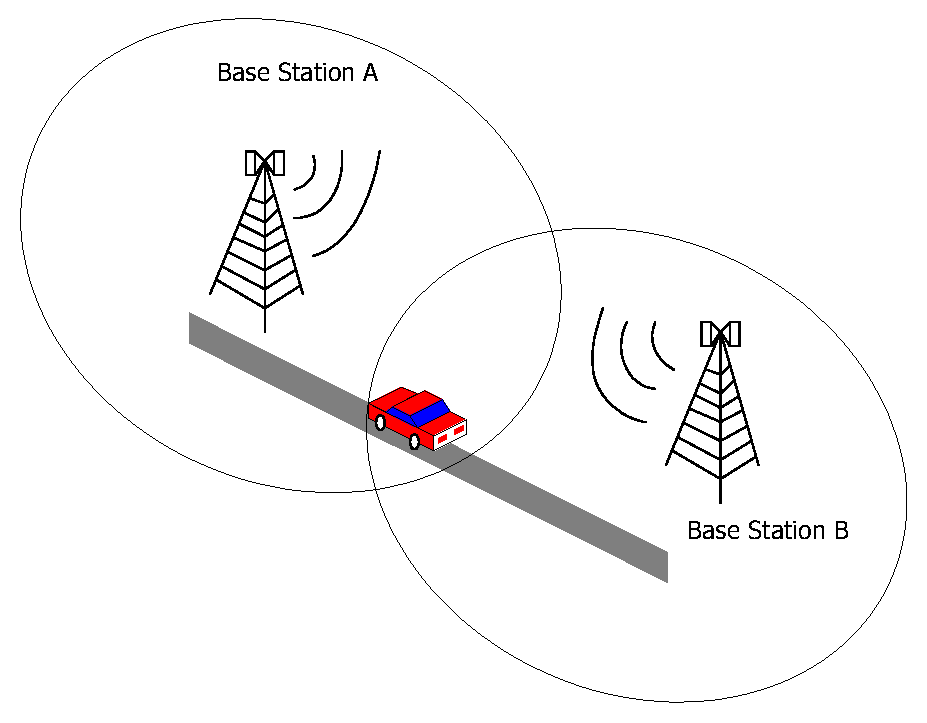
\includegraphics[height=6.75cm]{../figures/iccs_handover_bs}
%\caption{Simulation results of the probability of a handover success using the proposed adaptive FEC scheme.}
\caption{基站切换示意图}
\label{fig:chap_iccs_handover_bs}
\end{centering}
\end{figure}
%%%%%%%%%%%%%%%%%%%%%%%%%%%%%%%%%%%%%%%%%%%%%%%%%%%%%%%%%%%%%%%%%%%%%

当前的移动WiMAX标准详细定义了在切换过程中所需的切换信令协议。
这些协议被用来在单点到多点(Point-to-multipoint,PMP)模式的通信中支持切换过程。
通常,切换技术可以细分成两种:软切换(Soft handover, SHO)和硬切换(Hard Handover,HHO)。
在软切换过程中,移动台在切断与原有基站通信之前,就已经完成和目标基站的切换信令交换过程,并建立了正常的通信连接。
而在硬切换过程中,移动台先要完全断开与原有服务基站的连接,然后再与目标基站建立通信连接。
显然,软切换的优点在于在切换的过程中,数据连接始终存在。
但是同时资源利用率相比硬切换要低。
在硬切换过程中,数据连接会在一个小段时间内断开。
由此引入了一些延时,对于时间敏感的应用而言,需要做专门地处理和优化来确保通信服务质量。
此外,对于时间敏感的应用,软切换也会进行一些优化的处理才能保证在移动WiMAX中QoS。


近些年来,对于软切换方面的研究,许多学者做了大量工作。
一部分人的工作是集中在目标基站的选择策略上。
通过对移动台位置变化的预测、收集分析相邻基站的QoS信息或是对基站信号的分析来优化目标基站的选择\cite{Hsieh:INFOCOM2003}\cite{DooHwan:WPC2006}。
另外一些人的工作主要是集中在提高某些QoS的指标。
例如,学者Minsiki为了解决在切换过程中丢包率增加的问题,采用交叉层的设计方法。他们在上层设备中,如网络层中的路由器,缓存切换用户的数据\cite{MinsikICACT2006}。
Chen等学者为了减少切换过程中的延时,提出了一种预协商的机制。
这个机制利用预测移动台与基站间的距离,提前在目标基站中分配所需要的资源\cite{JenHui:AUSWIRELESS:2007}。
学者Ling通过用IP层的链路来传送MAC层的信息来达到减少切换延时的目的\cite{LingVTC2007}。
还有一些学者的研究集中在切换过程中出现的CID(Connection Identifier) 分配冲突,提出了更为合理的分配方案,或是对移动台的数据进行分类处理,最终也可以提高QoS的水平\cite{Hu:TVT2004}\cite{Wenhua:ICC2007}。


以往的大部分工作主要是从数据链路层或IP层来考虑切换的性能。他们的工作一般是假设无线信道是一个理想信道。在本章中,我们认为如果物理层的信道工作能与数据链路层工作进行协调,就可以有效提高切换性能。特别是在移动台高速运动的状态下。
下面,我们将会分析信道质量对切换信令交换流程的影响。
然后,通过建立信令交换的概率模型来分析在高速移动状态时的切换性能。
最后通过建立一个简单实用的自适应前向纠错方法来提高切换的成功率和效率。


\section{基站切换成功概率模型}
\label{section_iccs_handover_algorithm_mobility_analysis}
\esection{Probability Model of Handover}
切换的性能与效率通常可以用一个切换的成功率来描述。我们通过统计在切换过程中每次信令的交换成功概率来计算出完成整个切换过程概率。
在高速运动的切换过程中,移动速度会对切换造成非常大的影响。它不但反映移动台切换延时情况,也在研究切换用户丢包模型中扮演着重要的角色。
\subsection{切换的流程建模分析}
\esubsection{Hanover Protocols in WiMAX}
\label{subsection_iccs_handover_algorithm_mobility_analysis_handover_flow}
在IEEE 802.16e的标准中,切换信令的交换流程如图\ref{fig:chap_iccs_handover_algorithm_handover_flow}所示。
基站会周期地广播“邻近通告消息”(Neighbor Advertisement Message, MOB\_NBR-ADV)。
这个消息用来标识邻近基站或是它们的信道特征。
移动台总是会侦听此消息来收集邻近基站的信息。
如果一个移动台检测到与当前服务基站的信道变差,它会发送一个请求消息(MOB\_SCAN-REQ)给当前服务的基站。
如果基站收到此请求消息后,会反馈给移动台一个消息(MOB\_SCAN-RSP)。
此消息会指示移动台使用特定的无线资源(如时隙)来进行扫描操作(Scanning),确定目标基站。
当扫描操作结束后,移动台初始化切换过程,发送切换请求消息(MOB\_MSHO-REQ)给当前基站。
然后基站会发送响应消息信令(MOB\_BSHO-RSP)。
当移动台收到此消息时,它会发送消息(MOB\_HO-IND)通知当前基站可以关闭此移动的连接,释放无线资源。
(如果是硬切换,移动台会中断与当前服务基站的连接。如果是软切换,连接会继续保留直到与目标基站的信令交换结束。)
最后,移动台与目标基站交换测距消息以及重新接入的各种信令来完成剩余的切换流程。
综合上述的描述,一次成功的切换过程,尽管无线资源的分配也是切换需要考虑的内容,
但从数据链路层的信令层面上看,其核心首先是各种切换信令的成功传递与交换。

%%%%%%%%%%%%%%%%%%%%%%%%%%%%%%%%%%%%%%%%%%%%%%%%%%%%%%%%%%%%%%%%%%%
\begin{figure}[t]
\centering
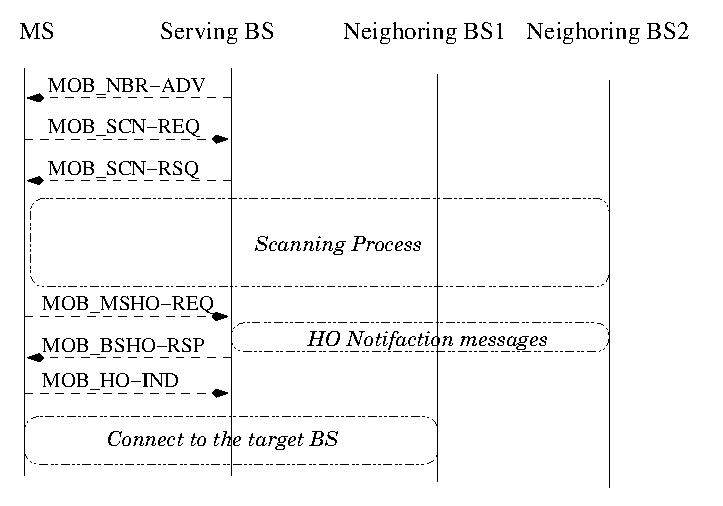
\includegraphics[height=7.75cm]{iccs_handover}
\caption{切换流程示意图}
%\caption{Illustration of the handover procedure.}
\label{fig:chap_iccs_handover_algorithm_handover_flow}
\end{figure}
%%%%%%%%%%%%%%%%%%%%%%%%%%%%%%%%%%%%%%%%%%%%%%%%%%%%%%%%%%%%%%%%%%%

\subsection{切换成功概率建模与误比特率}
\esubsection{Probability of Handover Success and Bit Error Rate}
根据上面的分析,我们考虑一个这样的切换过程模型。
不失一般性,我们假设在一次移动台的切换过程中有~$M$~($M \ge 2 $)个信令需要交换。
设事件~$A_i$~表示一次信令的传送。
 ~$p_i$~是此次信令成功传送的概率,其中 ~$i = 0,1, \cdots, M-1 $~。
如果不考虑自动重传(ARQ)的策略,则有以下结论:
%%%%%%%%%%%%%%%%%%%%%%%%
\begin{equation}
\label{eq:chap_iccs_handover_algorithm_pro_mess_no_tran}
\begin{cases}
P(A_{i})=p_{i}\\
P(\bar{A}_{i})=1- p_{i}
\end{cases}
\end{equation}
%%%%%%%%%%%%%%%%%%%%%%%%
其中,~$i=0,1,\cdots,M-1$~。
接下来我们分析一下有重传策略的情况。
在切换过程中,重传策略不但可以用于用户数据的传递,也可用于保证信令消息的可靠传送。
所以,根据切换信令的要求,这里我们假设一个信令消息如果不能被对方成功接收,将会被重传定时器激发重新发送过程,并直到接到对方反馈为止。
那么,如果考虑了重传策略后,则公式 (\ref{eq:chap_iccs_handover_algorithm_pro_mess_no_tran})可以重新写为下面的式子:
%%%%%%%%%%%%%%%%%%%%%%%%
\begin{equation}
\label{eq:chap_iccs_handover_algorithm_Pro_basic01}
P(A_{i})=\sum_{j=1}^{N_{i}}q_{i}^{j-1}p_{i}=\sum_{j=1}^{N_{i}}
(1-p_{i})^{j-1}p_{i},\quad N_{i}\geq1,
\end{equation}
%%%%%%%%%%%%%%%%%%%%%%%%
其中,~$N_i$~表示在一次切换过程中,第~$i$~个信令消息在成功接收前被传递的次数。在切换过程中有~$M$~个信令消息,那么,只有~$M$~个信令都成功收到,切换才认为是成功的,所以切换成功的概率可表示为:
%%%%%%%%%%%%%%%%%%%%%%%%%%
\begin{equation}
\label{eq:chap_iccs_handover_algorithm_Pro_basic02}
P_{succ}=\prod_{i=0}^{M-1}P(A_{i})=\prod_{i=0}^{M-1}
\left[\sum_{j=1}^{N_{i}}(1-p_{i})^{j-1}p_{i}\right].
\end{equation}
%%%%%%%%%%%%%%%%%%%%%%%%%%
因为当前通信系统的物理层中普遍采用交织信道编码的技术,所以模型中的无线信道可以假设为无记忆的信道。那么,概率~$p_i$~将主要与移动台和基站之间的无线信道的误比特率有关。我们用数学公式表示如下:
%%%%%%%%%%%%%%%%%%%%%%%%%%
$$
p_{i}=\varphi(P_{b}(\gamma_{b}),\: L_{i}),
$$
%%%%%%%%%%%%%%%%%%%%%%%%%%
其中,~$P_b(\gamma_b)$~是当接收比特信噪比为~$\gamma_b$~的误比特概率。这样,如果设第~$i$~个信令消息的长度为~$Li$~,则有
%%%%%%%%%%%%%%%%%%%%%%%%
\begin{equation}\label{eq:chap_iccs_handover_algorithm_Pro_basic03}
p_{i}=[1-P_{b}(\gamma_{b})]^{L_{i}}.
\end{equation}
%%%%%%%%%%%%%%%%%%%%%%%%
所以,将公式(\ref{eq:chap_iccs_handover_algorithm_Pro_basic03})代入公式(\ref{eq:chap_iccs_handover_algorithm_Pro_basic02}),可以得到切换模型中的切换成功概率与无线信道误比特率之间的关系。
%%%%%%%%%%%%%%%%%%%%%%%%%
\begin{align}
\label{eq:chap_iccs_handover_algorithm_Pro_basic_final}
\notag P_{succ}&=\prod_{i=0}^{M-1}P(A_{i})\\
&=\prod_{i=0}^{M-1}\left\{ \sum_{j=1}^{N_{i}}\left\{ 1-[1-P_{b}(\gamma_{b})]^{L_{i}}\right\} ^{j-1} \cdot[1-P_{b}(\gamma_{b})]^{L_{i}}\right\}
\end{align}
%%%%%%%%%%%%%%%%%%%%%%%%%%
%%%%%%%%%%%%%%%%%%%%%%%%%%%%%%%%%%%%%%%%%%%%%%%%%%%%%%%%%%%%%%%%%%%%%
\begin{figure}[t]
\begin{centering}
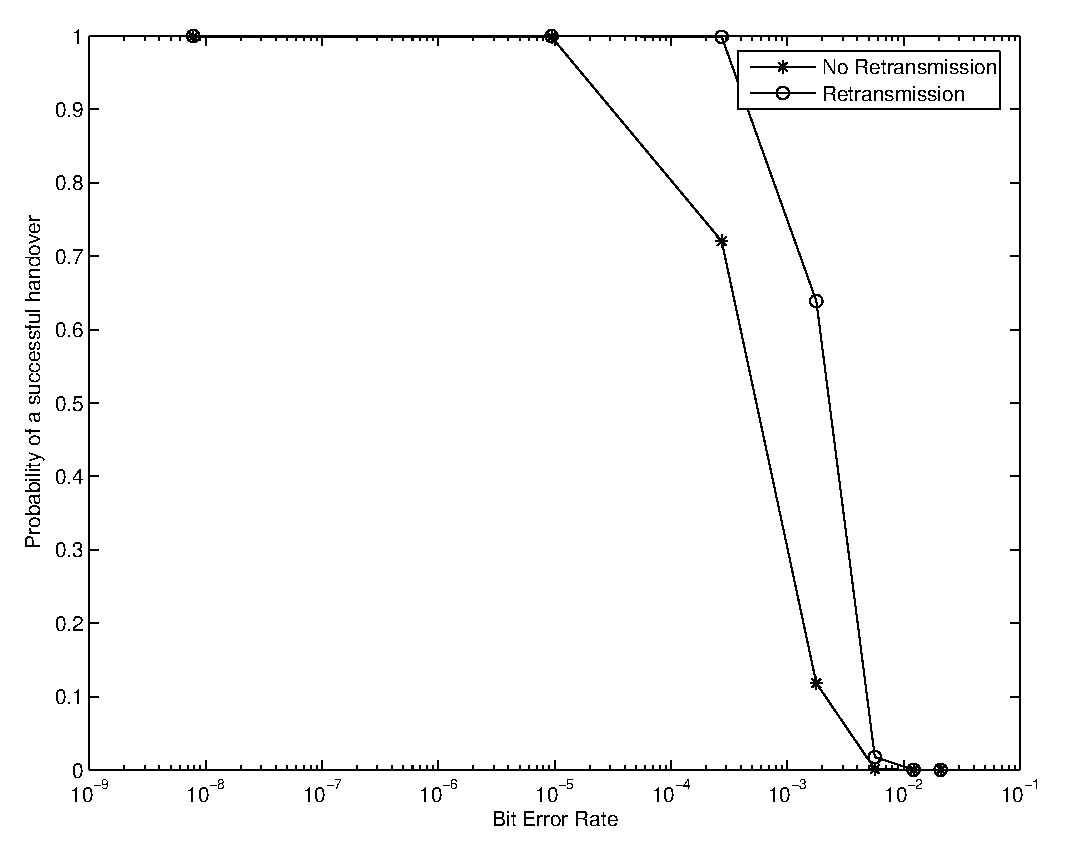
\includegraphics[height=7.75cm]{iccs_ber_prob}
\par\end{centering}
%%\caption{Probability of a handover success as a function of BER, where ~$M=5,\sum_{i=0}^{M-1}N_i<=50,L_i=250$~ bits in this case.}
\caption{切换成功概率与误比特率的关系。在此例中,~$M=5,\sum_{i=0}^{M-1}N_i<=50,L_i=250$~}
\label{fig:chap_iccs_handover_algorithm_PBER}
\end{figure}
%%%%%%%%%%%%%%%%%%%%%%%%%%%%%%%%%%%%%%%%%%%%%%%%%%%%%%%%%%%%%%%%%%%%%
这里,我们给出公式(\ref{eq:chap_iccs_handover_algorithm_Pro_basic_final})的一个例子,如图 \ref{fig:chap_iccs_handover_algorithm_PBER} 所示。
可以明显地看出,对于固定的~$N_i$~,切换的成功概率~$P_{succ}$~随着误比特概率~$P_b(\gamma_b)$~的增大而降低。当误比特率较大时(在~$10^{-4}$~到~$10^{-2}$~之间),使用重传策略会有效地改善切换的成功率。

\subsection{切换成功概率模型与移动台速度}
\esubsection{Probability of Handover Success and Velocity of MS}
上一节的分析指出了切换成功概率与两个重要的参数有关:一是信道的误比特率,二是信令消息的重传次数。
在一个实际的WiMAX网络中,这二者都与移动台的移动速度有关。
首先,移动的速度会影响多谱勒频率偏移,进而影响信道的误比特率,最终对信令消息的重传次数产生影响。
其次,两个相邻基站覆盖的交叠部分的物理距离有限,因而不能做到无限制的重传。
所以,一个快速移动的终端要求基站切换的速度与时间也有更严格的要求。
基于上述的考虑可知,通常情况下,移动台的移动速度越快,切换成功的概率会越低。

为了定量的分析起见,我们假设在切换过程中,对信令处理的时间可以忽略不计的。
所以,在整个切换过程中的延时可以写为下面的式子,
%%%%%%%%%%%%%%%%%%%%%%%%%%%%%%%%%%%%%
$$
T_{M}=(N_{0}+N_{1}+\cdots+N_{M-1})\cdot T_{retx}+M\cdot T_{prop},
$$
%%%%%%%%%%%%%%%%%%%%%%%%%%%%%%%%%%%%%
其中,~$N_i$~表示第~$i$~个信令传递的次数。~$T_{retx}$~是同一信令消息重传的计时器间隔,~$T_{prop}$~是在移动台与基站之间的承载信令的电磁波传播所需时间。

我们用~$D_{overlap}$~表示在移动台移动方向上两个相邻基站覆盖范围重叠部分的距离。
如图\ref{fig:chap_iccs_handover_bs}如示。
$v_m$是移动台的移动速度。
因此,在一次成功的基站切换过程中,需要满足下面的时间约束\eqref{eqn:chap_handover:times_T_M}:
%%%%%%%%%%%%%%%%%%%%%%%%%%%%%%%%
\begin{equation}
T_{M}<\frac{D_{overlap}}{v_{m}}.
\label{eqn:chap_handover:times_T_M}
\end{equation}
%%%%%%%%%%%%%%%%%%%%%%%%%%%%%%%
在这个约束下,一次成功切换的概率可以进一步被改写\eqref{eq:chap_iccs_handover_algorithm_Pro_basic_final00},

%%%%%%%%%%%%%%%%%%%%%%%
\begin{equation}
P_{succ}=\left\{
\begin{array}{ll}
\prod_{i=0}^{M-1}\left[\sum_{j=1}^{N_{i}}(1-p_{i})^{j-1}p_{i}\right],
& \mbox{if }T_{M}<\frac{D_{overlap}}{v_{m}},\\
\\0, & \mbox{others},
\end{array}\right.\label{eq:chap_iccs_handover_algorithm_Pro_basic_final00}
\end{equation}
%%%%%%%%%%%%%%%%%%%%%%%
其中,
%%%%%%%%%%%%%%%%%%%%%%%%
\begin{align*}
T_{M}=\sum_{i=0}^{M-1}(N_{i})\cdot T_{retx}+M\cdot T_{prop} \\
p_{i}=[1-P_{b}(\gamma_{b})]^{L_{i}}
\end{align*}
%%%%%%%%%%%%%%%%%%%%%%%%
这里,假设使用Rayleigh信道。平均接收符号的信噪比(energy-to-noise)可以表示为:\cite{GLST:PMC2002}\cite{Leung:WCNC2005}
%%%%%%%%%%%%%%%%%%%%%%%%
\begin{equation}
\bar{\gamma}_{s}=\frac{1}{1-\frac{1}{N^{2}}\left[N+2\sum_{i=1}^{N-1}\left(N-i\right)J_{0}(2\pi f_{m}T_{s}i) \right]
+\frac{NT_{s}}{E_s/N_{0}}},
\end{equation}
%%%%%%%%%%%%%%%%%%%%%%%
其中,~$N$~是OFDM子载波的个数,~$T_s$~是一个K阶QAM调制的符号在一个子载波上的传输时间。~$N_0$~是噪声功率, ~$E_s$~是传送每个符号的平均能量。~$f_{m}=fv_{m}/c $~是最大的多谱勒频偏,~$f$~为载波频率,~$v_m$~为移动台的速度,~$c$~为光速。那么相应的接收到的平均比特信噪比为
%%%%%%%%%%%%%%%%%%%%%%%%
\begin{align}
\bar{\gamma}_{b}&= \frac{ \bar{\gamma}_s} {\log_2K} \notag\\
&=\frac{1/\log_{2}K}{1-\frac{1}{N^{2}}\left[N+2\cdot \sum_{i=1}^{N-1}\left(N-i\right) J_{0}(2\pi f_{m}T_{s}i) \right]
+\frac{NT_{s}}{\log_{2}K}\left(\frac{1}{E_{b}/N_{0}}\right)}
\label{eqn:chap_handover:avg_snr}
\end{align}
其中,
\begin{equation*}
J_{0}(2\pi f_{m}T_{s}i) = \frac{1}{\pi}\int_0^\pi \cos(2\pi f_m T_{s}i \sin \theta) d \theta
\end{equation*}
%%%%%%%%%%%%%%%%%%%%%%%
此处,我们假设以Clarke-Jakes的模型为基础的Rayleigh信道模型。

%其中,~$Y$~定义为
%%%%%%%%%%%%%%%%%%%%%%%%
%$$
%Y=\sum_{i=1}^{N-1}\left(N-i\right)J_{0}(2\pi f_{m}T_{s}i)
%$$
%%%%%%%%%%%%%%%%%%%%%%%%%
对于K阶的QAM调试(如果~$K=4$~,调制的方式是QPSK;如果~$K=16$~,那么就是16-QAM)。
我们假设在接收端可以进行出错的符号检测。那么对于当接收比特能量与噪声比为~$\gamma_b$~时,误比特概率(bit error, BER)为~$P_b(\gamma_b)$~可以写为:
%%%%%%%%%%%%%%%%%%%%%%%
\[
{{P}_{b}}=\int\limits_{0}^{\infty }{{{P}_{b}}(\gamma ){{f}_{{{\gamma }_{b}}}}(}\gamma )d\gamma
\]
%%%%%%%%%%%%%%%%%%%%%%%%
其中,~$f_{\gamma_b}$~是Rayleigh信道模型的比特能量与噪声比的概率密度函数。它定义如下:
%%%%%%%%%%%%%%%%%%%%%%%%%
\[{{f}_{{{\gamma }_{b}}}}(\gamma )=\frac{\exp (\frac{-\gamma }{{{{\bar{\gamma }}}_{b}}})}{{{{\bar{\gamma }}}_{b}}},\gamma \ge 0\]
%%%%%%%%%%%%%%%%%%%%%%%%%%%%
我们假设载波间的干扰(ICI)为高斯白噪声。这个值近似在~$256 \le N \le 1024$~是比较精确的\cite{Leung:WCNC2005}。那么,对于K阶的QAM和Gray码,可以有如下的近似,
%%%%%%%%%%%%%%%%%%%%%%%
\begin{equation}
P_b(\gamma_b) \approx \frac{P_M(\gamma_s)}{\log_2 K}
\end{equation}
%%%%%%%%%%%%%%%%%%%%%%%
其中,~$P_K$~是符号的错误概率。特别对于QPSK,有
%%%%%%%%%%%%%%%%%%%%%%%%
\begin{align}
\label{eq:chap_iccs_handover_algorithm_BER_V}
P_{b}(\gamma_{b})&= Q\left(\sqrt{2\gamma_{b}}\right).\\
Q(x) &= \int^x_{-\infty} \frac{1}{\sqrt{2\pi}}e^{-y^2/2}dy \notag
\end{align}
%%%%%%%%%%%%%%%%%%%%%%%%
把公式(\ref{eq:chap_iccs_handover_algorithm_Pro_basic_final00})和公式( \ref{eq:chap_iccs_handover_algorithm_BER_V})合并则有下面的结果。
%%%%%%%%%%%%%%%%%%%%%%%
\begin{equation}
P_{succ}=\left\{
\begin{array}{ll}
\prod_{i=0}^{M-1}\left[\sum_{j=1}^{N_{i}}(1-Q\left(\sqrt{2\gamma_{b}}\right))^{j-1}Q\left(\sqrt{2\gamma_{b}}\right)\right],
& \mbox{if }T_{M}<\frac{D_{overlap}}{v_{m}},\\
\\0, & \mbox{others}
\end{array}\right.\label{eq:chap_handover:velocity_bit_error_rate}
\end{equation}
其中,~$\gamma_b$~是移动速度的一个函数。
至此,我们可以得到以移动台速度为变量的一个切换成功概率函数模型。其函数图形,如图\ref{fig:chap_iccs_handover_algorithm_Pro_V} 所示。
%%%%%%%%%%%%%%%%%%%%%%%%%%%%%%%%%%%%%%%%%%%%%%%%%%%%%%%%%%%%%%%%%%%%
\begin{figure}[t]
\begin{centering}
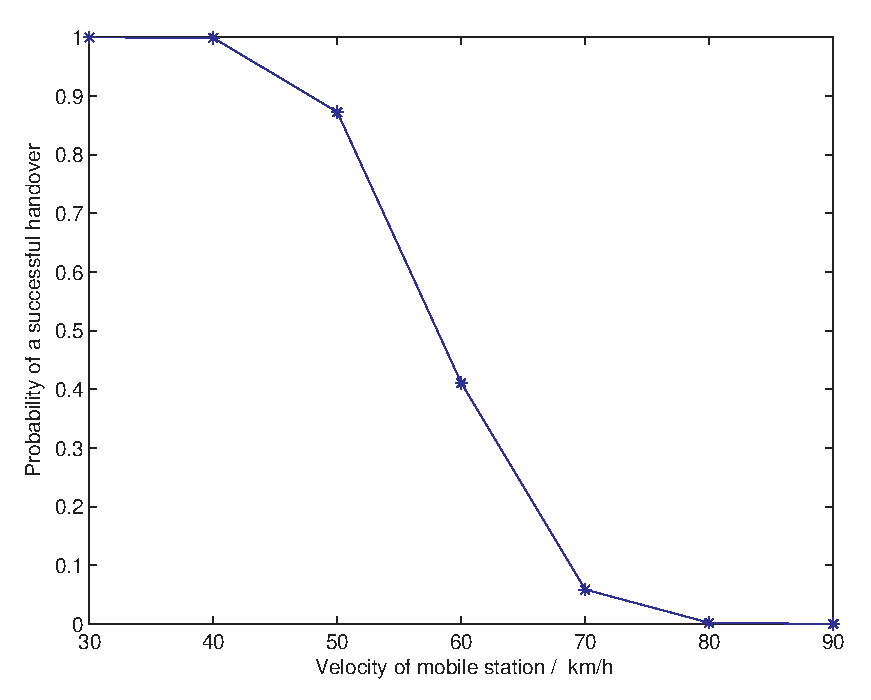
\includegraphics[height=7.75cm]{iccs_speed_prob_theroy}
%%\caption{The probability of a handover success as a function of MS's velocity, where ~$M=5, \sum_{i=0}^{M-1}N_i=50, L_i=250$~ bits in this case.}
\caption{切换成功概率与用户的移动速度关系,在本例中~$M=5, \sum_{i=0}^{M-1}N_i=50, L_i=250$~}
\label{fig:chap_iccs_handover_algorithm_Pro_V}
\end{centering}
\end{figure}
%%%%%%%%%%%%%%%%%%%%%%%%%%%%%%%%%%%%%%%%%%%%%%%%%%%%%%%%%%%%%%%%%%%%

从图中可明显看出,随着移动的速度增快,切换成功概率会显著下降。这样会极大地影响了切换的过程。所以说,如果在高速移动状态下,切换对于移动台来说需要额外的处理。

\section{基于切换成功概率模型的切换方案}
\esection{Handover Scheme with High Velocity MS}
在高速移动状态下,为了提高移动台的切换成功概率,除了可以减小重传间隔、增加重传的次数以外,我们也需要建立更加可靠的通信链路的传输机制来传送信令消息。
本节我们讨论了前向纠错编码的特点,并采用此技术来改善传输的误码率。
前向纠错编码是通过发送端使用冗余比特数来提供差错保护。
这些额外的冗余比特可以帮助接收端检测并纠正错误。
如果采用了前向纠错的技术,数据重传的次数也会降低。
根据WiMAX的标准,切换信令的消息大小约为50到180个字节左右。

不同的前向纠错编码方案可以提供不同的纠错能力。
对于同一种前向纠错码而言,冗余比特数越多,纠错能力也超强。
同时由于无线信道的限制及交换的信令消息较多,所以要在满足设计要求的基础上尽可能减少冗余比特数。

因此,下面我们定量地讨论冗余比特的个数。对于一个给定的移动台速度,我们要能基于系统设计要求达到的切换成功率来计算出冗余比特数。为了简单起见,我们使用切换消息信令的平均长度,设切换消息传输一次的成功的概率为~$\tilde{p}$~以替换公式(\ref{eq:chap_iccs_handover_algorithm_Pro_basic_final00})中的~$p_i$~,如下
%%%%%%%%%%%%%%%%%%%%%%%%%%%%%%%%%%%
\begin{align}
\notag P_{succ} &= \prod_{i=0}^{M-1}P(A_{i})\\
&= \prod_{i=0}^{M-1}\left[\sum_{j=1}^{N_{i}}(1-p_{i})^{j-1}p_{i}\right]\\
\notag &\thickapprox\sum_{i=M}^{S}{i-1 \choose M-1}\cdot\widetilde{p}^{M}(1-\widetilde{p})^{i-M}
\end{align}
%%%%%%%%%%%%%%%%%%%%%%%%%%%%%%%%%%
其中,~$S=\sum_{i=0}^{M-1}N_{i}$~是总共重传的次数。根据前面小节的分析,可以得到如下的公式:
%%%%%%%%%%%%%%%%%%%%%%%%%%%%%%%%%%
\begin{align*}
S & = \sum_{i=0}^{M-1}N_{i}\\
  & = \left\lfloor \frac{(\frac{D_{overlap}}{v_{m}}-MT_{prop})}
        {T_{retx}}\right\rfloor \leq\frac{(\frac{D_{overlap}}{v_{m}}
        -MT_{prop})}{T_{retx}}.
\end{align*}
%%%%%%%%%%%%%%%%%%%%%%%%%%%%%%%%%%
这样,我们就可根据相邻基站覆盖交叠的距离~$D_{overlap}$~和移动台的速度~$v_m$~,得到参数~$S$~;并根据系统设计要求的~$P_{succ}$~进一步计算得每一个信令的成功传输的概率值。如果使用Reed-Solomon(R-S)纠错编码,我们可以推导出如下\eqref{eq:chap_iccs_handover_algorithm_FEC_Pro_final}。
%%%%%%%%%%%%%%%%%%%%%%%%%%%%%
\begin{equation}\label{eq:chap_iccs_handover_algorithm_FEC_Pro_final}
\tilde{p}\approx\frac{2^{k-1}}{k(2^{k}-1)^{2}}\sum_{j=t+1}^{2^{k}-1}j
\cdot{2^{k}-1\choose j}_{}^{}\cdot p^{j}(1-p)^{2^{k}-1-j},
\end{equation}
%%%%%%%%%%%%%%%%%%%%%%%%%%%%%
其中, ~$t=\lfloor\frac{N-k}{2}\rfloor$~ 是编码的符号纠错能力,~$N$~是全部的比特数,~$k$~是信令消息的比特数, ~$\lfloor{x}\rfloor$~表示不超过~$x$~的最大整数。那么冗余比特数~$N-k$~可以确定下来。图 \ref{fig:chap_iccs_handover_algorithm_AFEC_bits} 表明了在切换流程要达到不同的切换成功概率(~$50\%,80\%,99\%$~)下,在不同的速度下,移动台切换所需的冗余比特数。
%%%%%%%%%%%%%%%%%%%%%%%%%%%%%%%%%%%%%%%%%%%%%%%%%%%%%%%%%%%%%%%%%%%%%%%%%%%
\begin{figure}[t]
\begin{centering}
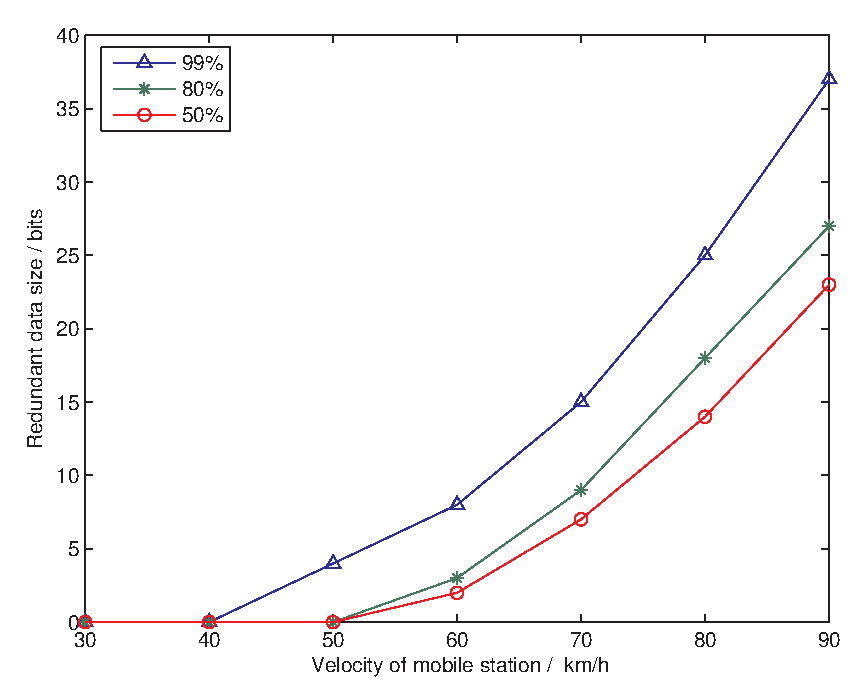
\includegraphics[height=6.75cm]{iccs_speed_size_theory}
\caption{RS码中的冗余比特数与移动台速度之间的关系,其中,假设~$k=250$~比特}
\label{fig:chap_iccs_handover_algorithm_AFEC_bits}
\end{centering}
\end{figure}
%%%%%%%%%%%%%%%%%%%%%%%%%%%%%%%%%%%%%%%%%%%%%%%%%%%%%%%%%%%%%%%%%%%%%%%%%%%

如图 \ref{fig:chap_iccs_handover_algorithm_AFEC_bits}所示,当移动台的速度越快,那么为了达到系统设定的切换成功概率,所需的冗余比特数也越多。例如,为了能够达到~$80\%$~的成功概率,如果移动台的速度分别是50,70, 90 km/h,那么所需的冗余比特数是2,10,28。通过上面的分析,我们可以使用一种自适应的方法根据不同的移动台速度来增加所需的冗余比特。

\section{仿真实验与结果分析}
\esection{Simuation and Results}
我们通过计算机仿真实验来验证和评估我们的切换概率模型及相应的前向纠错方案。在实验中,我们使用了NS-2仿真模拟器和修改了的NIST的WiMAX仿真代码\cite{NS2_simulator}\cite{NIST_WIMAX}。实验主要的实验设置参数如表格\ref{chap_iccs_table_I} 所示。

%%%%%%%%%%%%%%%%%%%%%%%%%%%%%%%%%%%%%%%%%%%%%%%%%%%%%%%%%%%%%%%%%%%%%
\begin{table}[htbp]
\wuhao
\centering
%\begin{centering}
\caption{仿真实验的主要参数配置}\label{chap_iccs_table_I}
\begin{tabular*}{0.99\textwidth}{p{7cm} p{7cm}} 
\toprule 
参数名称  & 参数值 \\
\midrule
移动方向上的交叠距离  & 200 米\tabularnewline 
带宽  & 5 MHz\tabularnewline 
载波频率  & 2.5 GHz\tabularnewline 
FFT   & 512\tabularnewline
信道类型  & Rayleigh channel\tabularnewline 
FEC  & Reed-Solomon code\tabularnewline 
移动速度  & 30-90 km/h\\
\bottomrule
\end{tabular*}
%\end{centering}
\end{table}
%%%%%%%%%%%%%%%%%%%%%%%%%%%%%%%%%%%%%%%%%%%%%%%%%%%%%%%%%%%%%%%%%%%%%

这里,我们采用的是自适应的前向纠错码方案。
冗余比特数是理论计算事先得到的。
在切换成功概率为50\%,80\%,99\%的情况下,计算出所需要的冗余比特数。
对于每一组实验参数,仿真进行100次,然后取结果的平均值来得到最后的统计结果。
最终得到的仿真实验结果,如\figref{fig:chap_iccs_results}所示。
从图中我们可以看到,在移动台的速度较低时,少量增加一些冗余比特会使得切换成功的概率会显著增加,并接近于~1。
而当速度逐渐增大后,对于目标为50\%的曲线,切换成功率会下降,但仍然会保持在50\%以上。
这说明,在保证高切换成功率,如99\%,所增加的冗余比特数较多,我们的方案略显些保守。
而且我们也注意到,在速度为70km/h时,理论成功率50\%的曲线存在一个局部极值点。
经过反复实验与比对,我们认为有两个原因会造成:
一是,在NS2系统中的Rayleigh信道模型计算误比特数时存在偏差。
二是,\eqref{eqn:chap_handover:avg_snr}中速度与SNR关系偏差所致。

%%%%%%%%%%%%%%%%%%%%%%%%%%%%%%%%%%%%%%%%%%%%%%%%%%%%%%%%%%%%%%%%%%%%%
\begin{figure}[t]
\begin{centering}
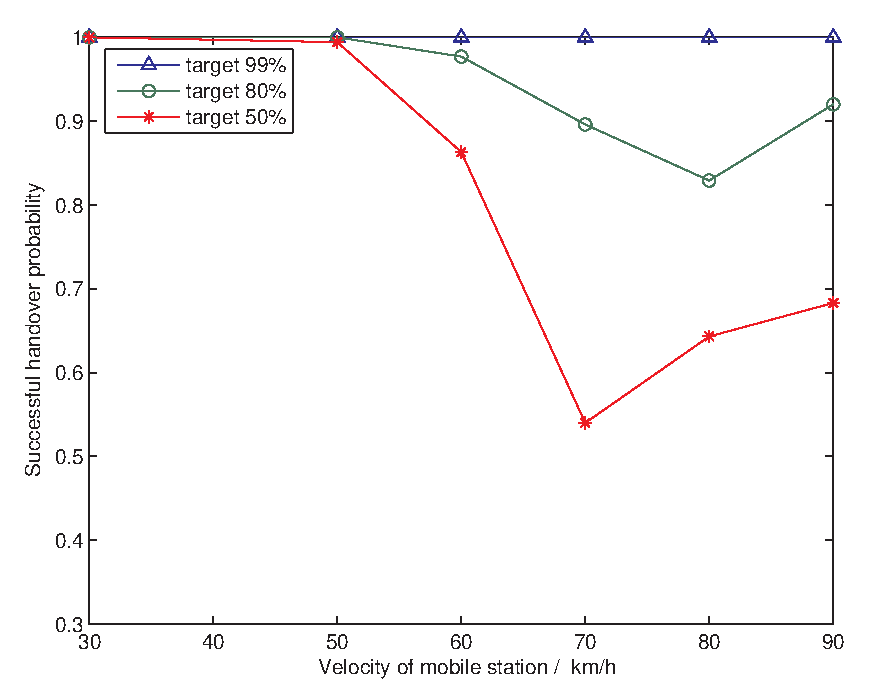
\includegraphics[height=7.75cm]{iccs_speed_prob_simu}
%\caption{Simulation results of the probability of a handover success using the proposed adaptive FEC scheme.}
\caption{仿真实验的结果}
\label{fig:chap_iccs_results}
\end{centering}
\end{figure}
%%%%%%%%%%%%%%%%%%%%%%%%%%%%%%%%%%%%%%%%%%%%%%%%%%%%%%%%%%%%%%%%%%%%%

\section{本章小结}
\esection{Chapter Summary}
在本章中,我们以WiMAX网络为例分析了移动台的移动速度对切换成功率的影响。分析的结果表明,由于移动台的速度增加会导致无线传输的信道变差,进而使得切换信令不能正常收发。又由于切换操作是时间受限的,所以在设计切换时要两方面同时考虑。根据理论分析,我们提出了一个简单有效的自适应前向纠错方案,通过理论计算就可以得到在不同速度下所需的冗余比特数,可以满足在不同移动速度下的切换设计需求。最后仿真实验验证了我们的理论模型和所提出的前向纠错方案的正确性。
%chapter_end

%
%chapter_cacop_begin
\graphicspath{ {../body/cacop_figures/}}
\chapter{基于多媒体特性的呼叫接纳控制算法研究}
\label{chap_cacop}

从目前无线网络通信的发展趋势看,多媒体数据业务将会逐渐取代目前无线通信中话音业务为主的状况。
为了迎合这种发展趋势,新制定的无线通信标准也已经开始部分地支持多媒体业务数据的传输。比如,在IEEE802.16e中定义多媒体数据的调度类型。
原有的呼叫接纳控制算法显然不能满足多媒体无线通信的要求。
本章针对这一问题,首先细致地分析了多媒体业务的数据特点,并提出了不同业务类型的服务质量(QoS)水平的归一化定义方法。
然后根据这一定义提出了以系统服务质量及效用最优的呼叫接纳控制原则,以及其相应的接纳控制算法。

\section{前言}
呼叫接纳控制本质是一个管理呼叫连接并进行资源分配与管理的技术。
这项技术以往常常在无线话音网络,如GSM网络,或VoIP(Voice over Internet Protocol)的网络中使用\cite{Perros1996}\cite{Mase2004}
\cite{Systems_2001}\cite{Y-G-Fang.TVT.2002}\cite{Y-Xiao.IEICE.TC.2001}。
通常,这项技术也被看作是在有限的无线频谱资源与大量的资源需求之间的折衷策略。
比如,在电话服务网络中,由于业务对数据延时的敏感性,使得呼叫接纳控制单元,为了避免网络数据的拥塞不得不拒绝或阻塞一些话音呼叫的接入。
否则,已经拥塞的网络的状况会进一步恶化。
同时,呼叫接入控制又与网络资源的分配与管理密切相关。
例如,当某一个连接的数据流过于贪婪,占用了大量的网络资源时,
它会造成其它连接的业务服务质量下降,也会使得网络控制单元阻塞新的连接进入或中断现有连接的通信服务。
这都将使得接受网络服务的用户满意度下降。

到目前为止,研究人员提出了许多呼叫接纳控制的算法或方案。
这些算法中,有些是将基本的网络性能参数直接做为呼叫接纳的准则。
这些参数包括带宽资源利用率、单位时间内的数据包个数或在线呼叫个数等等。
当这些参数的值达到或超过了预先设置的上限或是下限,新的呼叫将会被迫延迟接入或是拒绝接入\cite{Y-Qian.TWC.2006} \cite{G-Djuka.TELSIK.2007}。
还有些算法是将一些底层(物理层或MAC层)参数加以合并,基于交叉层思想构造出新准则并应用于呼叫接纳控制。
例如,学者Song和Zhuang引入了一个被称之SRPT(shortest remaining processing time)的服务准则 \cite{Song2009}。
他们把一个时间窗的大小设置到一个合适的阈值来判断连接或呼叫是否可以被接入网络。
学者Yilmaz 和 Chen 则提出了一个类似商品买卖的竞价方案\cite{Yilmax2009}。
在这篇文献中,他们通过分析一个或多个数据流的特点将带宽资源标上价格,并设置价格的阈值。
通过使用一个或多个混合分区的价格阈值,可以周期地对资源进行定价来使系统的效用最大化。
对于那些不能负担资源费用的用户,会被系统拒绝接入或中断服务。
学者Zhai和Ni提出一个半马尔可夫决策过程来描述呼叫接纳过程 \cite{Zhai2005,Ni2009}。
他们把呼叫过程转化为一个求解系统资源利用最大化的数学问题。
学者Zhai和Xiang提出一个信道繁忙率(channel busyness ratio)的概念。
通过检测信道繁忙率来为呼叫接纳提供判断的准则 \cite{Zhai_Chen_Fang_2006}。
资源预留和优先级队列的思想也被许多研究者拿来解决呼叫接纳的问题。
例如,Chen和Kuo提出通过动态指派优先级的方法来接纳新呼叫 \cite{Chen_Kumar_Kuo_2003,Chen_Kuo_2004}。
学者Elsayed等人则使用了三种静态预留策略:统一预留、容量比例预留和剩余比例预留,并且做了详细的评估\cite{Elsayed02performanceevaluation}。
学者El-Kadi提出了动态预留方法 \cite{EL-Kadi2002}。
他在给新用户较高优先级的同时,采了“借和还”的预留策略。

在这些接纳控制文献中,对于接入判断准则及判断参数大多集中在物理层和MAC层上。
他们很少有人从多业务类型及网络应用层的角度,来研究呼叫接纳控制的判断准则。
这可能有两个原因:一个是以往无线网络承载的业务基本上以话音为主。其它的业务量的比重极小,几乎可以忽略不计。
二是虽然交叉层技术可以使得网络底层得到上层(如应用层)的部分信息,但是这样做的结果会破坏目前无线网络分层结构设计原则。
这使得交叉层技术的应用范围大打折扣。
本文的工作就是围绕这一问题展开的。
本章首先通过分析多媒体业务的数据特点,构造一个简单的服务质量水平映射评估模型,将应用层信息与底层参数信息做一个适当的映射关系。
然后,基于此模型,我们提出了自己的接纳控制及资源分配算法。这个新算法可以在兼顾资源利用效率同时,又可保证终端用户的服务质量。
%
\section{MAC层业务调度类型分类}
前面我们提到,随着网络业务的发展,新制定的无线通信标准也开始关注业务种类对通信质量的影响。
譬如,在WiMAX(Worldwide Interoperability for Microwave Access)中,
标准的制定者对MAC层数据包做了初步的分类\cite{Tsagkaris_Demestichas_2009}\cite{Andrews_Ghosh_Muhamed_2007}。
他们把数据分为五类:
每一类业务类型有自己相应的服务质量参数,例如延迟、抖动、丢包或错包率等等。
每一类数据的调度算法都应尽可能满足这些服务质量参数。
%但是同时,我们也注意到WiMAX的标准仅仅将这些数据分类而已,并没有说明如何调度这些已经分类的数据。这也给学者留下一块研究的空间。
此处我们引入WiMAX标准中数据调度类型定义,将业务分成以下几类。

\begin{itemize}
\item UGS(unsolicited grant service)业务:这种业务类型是指具有实时性要求的业务。
    其中,业务数据包具有周期性产生、包长固定的特点。
    比如T1、E1以及没有静默压缩的VoIP等就属于此类业务。
    这个特点使得UGS业务的数据流比较稳定,突发性不明显。
\item rtPS(real-time polling services)业务:这类业务也具有实时性要求,
    但是与UGS业务不同,它的数据包一般是变长的,同时也具有周期性。
    这类数据包的包头也比UGS数据包的包头要大。
    比如MPEG(Motion Pictures Experts Group)压缩的视频或H.264压缩视频流。
    在调度此类数据时,采用基站指导下移动台单播轮询策略(unicast polling)。
    基站需要通过提供足够多的轮询次数来保证业务的实时性要求。
\item nrtPS (non-real-time polling services)业务:
    顾名思义,这种业务与rtPS业务十分类似,但是对时延要求宽松。它采用的是移动台竞争轮询策略(contention-based polling)。
    如果在竞争轮询期间此类用户很多,资源申请冲突也会增多,需要使用冲突避让方案。
    所以,这种方式会引入较大的时间延迟。
\item BE (best-effort)业务:
    此类业务对服务质量的要求在几种业务类型中最低。往往也没有十分具体的QoS指标要求。
    如果能够申请到资源,就进行数据发送。如果不能,则继续等待下一次的调度。
    一般我们把普通的文字网页浏览,或是FTP文件的传送归于此类。
%\item ertPS(extended real-time polling service)业务:
%   这种业务类型是将上行数据链路的传输协议做了复用。
%   在传数据的同时,也可进行无线资源的申请。
%   这样可以保证数据量波动较大的情况下,资源能够得到及时的调度。
\end{itemize}

\section{呼叫接纳控制模型与业务流的QoS分析}
\label{sec_qos_metric}
因为不同的业务数据对服务质量的要求差别很大,所以要设计相应的传输机制来应对这种变化。
本节我们将详细描述如何将接纳控制算法与资源分配方案相结合。

%CAC
\subsection{呼叫接纳控制模型}
\label{sec_sec_model}
前面我们提到,呼叫接纳控制算法本质是为了避免网络拥塞,决策某一个呼叫或连接通信服务是否被中断或拒绝。
(因为名词“呼叫”一般专指话音通信,所以为避免文字概念混淆,下文一律用“连接(Connection)”一词来代替“呼叫(Call)”一词。)

此处,我们提出一个一般的呼叫接纳控制与资源分配控制的网络模型。
在此模型中,包括有一个基站(base station)和~$K$~个连接,如\ref{fig_system_model_cac}所示。
其中,包括在线的~$K-1$~个连接和~$1$~个正在申请进入的新连接。
这些连接根据不同的业务种类被分为四种类型,UGS,rtPS,BE,nrtPS。
在第~$K$~个连接被接入之前,所有 (~$K-1$~) 连接共享基站所提供的带宽资源,记为~$B_{total}$~。
当第~$K$~个连接进入基站的覆盖范围,并提交进入和资源需求的申请后,系统触发一次接纳控制的判断过程。
首先,服务质量评估单元(QoS Evaluator)会收集目前的连接情况,记为向量 ~$\mathbf{b} = (b_1, b_2, \dots, b_K)$~ 。
其中,~$b_i$~ 表示第~$i$~个连接所分配到的带宽,而且 ~$\sum_{i=1}^K b_i \le B_{total}$~。
然后,提交一份带宽资源新分配的方案,~$\mathbf{b^\prime} = (b_1^\prime, b_2^\prime, \dots, b_K^\prime)$~。
基于这个方案 ~$\mathbf{b^\prime}$~,接纳控制单元(Call Admission Control)根据每一个连接所分配到的带宽 ~$b_i$~来评估每一个连接的QoS水平,
同时也要评估整个系统的效用水平。
最后,接纳控制单元再决定接受或拒绝这个连接的进入请求。
%%
\begin{figure*}[t]
\centering
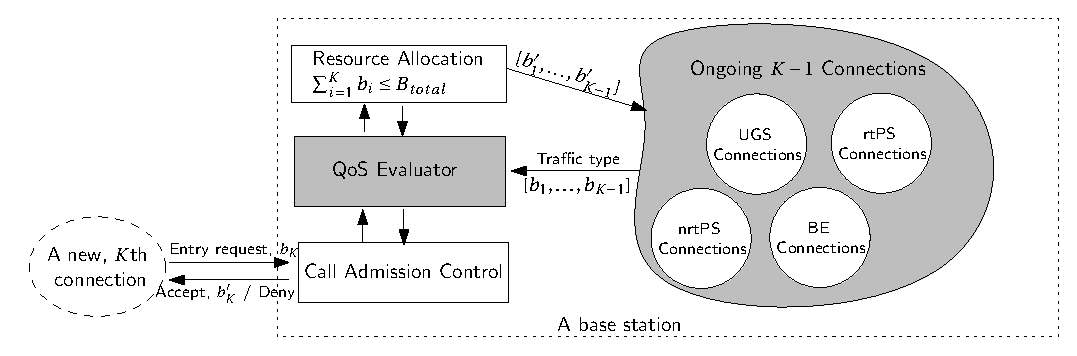
\includegraphics[width=0.95\textwidth]{cacop_qos_model_system.eps}
\caption{ 呼叫接纳控制的系统模型} \label{fig_system_model_cac}
\end{figure*}
%%%%%%
%QoS Metric
\subsection{带宽分配与QoS之间关系分析}
在以往的大多数文献中,也出现了一些关于接纳控制方面的QoS研究工作。
他们对用户或系统的QoS评价指标一般直接从网络底层,如物理层或MAC层,直接获得。
譬如,带宽资源的利用率、掉话率或呼叫中断概率等等。
但是很少有从应用层QoS来研究呼叫接纳控制的。
我们认为,对于用户从应用层感受到的QoS与底层网络QoS参数是区别的。
如果一个通信网络是以用户服务为中心的话,那么
对于业务连接的QoS评价也应该最好从应用层来评价。
但是,由于目前的通信网络是基于分层结构设计原则,上层如果需要传递给下层新的信息,就要大量修改或重新制定分层设计中的协议。
这对目前通信网络的结构冲击太大,会造成网络的大规模改造,显得有些不太切合实际情况。
因此,
我们提出可以通过一个预先认定的QoS的映射模型,利用底层所能获得的参数信息将上层QoS参数估计出来。
这样的话,就可以最大程度地兼容现有的通信网络。
对于业务连接而言,最重要的MAC层网络参数就是它们所分配到的带宽资源 ~$\mathbf{b}$~。
下面,我们结合具体的业务类型实例,对带宽资源与各项业务QoS之间的映射模型做详细的分析。

\begin{enumerate}[(1)]
    \item UGS业务与QoS评价:
        话音业务是UGS业务中最典型的一种。
        而ITU提出的E模型(E-Model)提供了一种可以客观评价话音传输服务质量的方法 \cite{ITU:G107}。
        此模型通过提取网络参数(如延时或丢包)定义了对话音评估的分析模型。
        E模型可以使用R因子(R-factor)来评价话音质量。一般,R因子的值域在~$0$~到~$100$~之间。
        ~$0$~表示话音质量最差;~$100$~表示话音质量最好。在有些文献中,R因子会简化为另一个常用的评价指标,MOS(Mean Opinion Score)。
        MOS用~$1$~到~$5$~来评价话音质量。~$1$~表示最差的质量,~$5$~表示最好的质量\cite{NK:IEICE:2005}。

        R因子的值可通过\eqref{eqn:chap_cacop:FactorR}计算得到:
\begin{equation}
\label{eqn:chap_cacop:FactorR}
R = R_0 − I_s − I_d − I_e + A 
\end{equation}
其中,~$R_0$~ 表示基本的信噪比(signal-to-noise ratio)。
~$I_s$~ 表示对于话音信号的损失之和。
~$I_d$~ 表示延时对通信的损害。
~$I_e$~ 表示由于低码率的编码方式对话音质量的影响。
~$A$~ 是一个优势因子(advantage factor),表示用户的容忍度。
为了计算方便,\eqref{eqn:chap_cacop:FactorR} 可以改写为经验\eqref{eqn:chap_cacop:FactorR_simple}
\begin{equation}
R = 93. 4 - I_d ( T_a ) -I_e ( codec, loss )
\label{eqn:chap_cacop:FactorR_simple}
\end{equation}
其中,~$I_d$~是一个单程延时函数。
(在我们例子中,我们假设延时较小可以被忽略。)
~$I_e$~ 代表编码器的类型及丢包情况。
我们通过E模型计算器来得到不同的丢包状况下的话音质量R因子的值\cite{ITU:EModel:Caculator}。 
结果如表\ref{tb:R_factor}所示。
从表中数据可以看出,话音业务对带宽资源极为敏感而且对丢包容忍度较低。
根据ITU提供的参考,R因子如果小于~$50$~则表明话音质量很差,用户很不满意。

\begin{table}[tb]
%\caption{R-Factor vs. Packet Loss} \label{tb:R_factor}
\caption{R因子与丢包率} \label{tb:R_factor}
\begin{center}
%\footnotesize
\begin{tabular*}{0.7\textwidth}{lcccccccccccc}
%\begin{tabular*}{0.5\textwidth}{lp{9mm}}
\toprule 
丢包率(\%):& 0& 0.1& 0.3& 0.5& 0.7& 0.9& 1& 2\\
R-因子: &93.2& 84.6& 71.3& 61.5& 54.1& 48.2& 45.2& 29.9\\ 
\bottomrule
\end{tabular*}
\end{center}
\end{table}

据此,我们尝试定义UGS业务的服务质量评估公式,如\eqref{eqn:chap_cacop:metric_voice}所示。
\begin{equation}
\label{eqn:chap_cacop:metric_voice}
\alpha^{UGS}=
\begin{cases}
1 & \text{if $b=B$,}\\
0 &\text{others}
\end{cases}
\end{equation}
其中,~$\alpha^{UGS}$~ UGS业务流的服务质量QoS的值。
~$b$~是所分配到的带宽;
~$B$~表示此话音连接根据业务需要,申请的带宽资源数量。
为了表示简洁,
我们改写为Delta函数的形式,
\eqref{eqn:chap_cacop:Dirac_UGS}.
%
\begin{equation}
\label{eqn:chap_cacop:Dirac_UGS}
\alpha^{UGS}= \delta_{b}(B) = 
\begin{cases}
1 & \text{if $b= B$,}\\
0 &\text{others}
\end{cases}
\end{equation}

\item rtPS业务与QoS评价: 
视频业务是一种典型的rtPS应用。
在视频传输或编码研究中,峰值信噪比(peak signal-to-noise ratio,PSNR)是最常见的视频质量评价方法。
它所采用的方法是将原始图像~$I$~与受损的重建图像~$K$~之间做逐像素的比较,
如\eqref{eqn:chap_cacop:psnr}所示。 
%
\begin{align}
\label{eqn:chap_cacop:psnr}
& PSNR = 10 \cdot \log_{10} \left( \frac{MAX_I^2}{MSE} \right)
\end{align}
其中,~$MAX_I$~ 是单个像素值域中的最大值。
如果每个像素点用~$8$~个比特表示,那么这个值就是~$255$~。
更一般的情况,如果每个像素采用~$z$~个比特表示,那么 ~$MAX_I$~就为 ~$2^z - 1$~。
分母部分是均方误差(mean squared error,MSE),表示原始图像~$I$~与解码重构图像~$K$~之间差。
它的定义为\eqref{eqn:chap_cacop:mse}。
%%%%%%
\begin{align}
\label{eqn:chap_cacop:mse}
MSE = \frac{1}{MN} \sum_{i=0}^{M-1}\sum_{j=0}^{N-1} \left[I(i,j) - K(i,j)\right]^2 
\end{align}
尽管PSNR在视频编码和解码研究领域广泛使用,但是它却不能直接在接纳控制单元中使用。
原因有两方面。一方面是,如果要想得到视频帧的PSNR的值,就要对压缩视频解码并恢复为YUV的图像帧。
这就意味着在MAC层中要嵌入视频解码单元。这一要求不太现实。
另一方面,PSNR的计算要有参考帧的图像。它是指原始压缩前的视频图像。
在一个通信网络中,这些数据对于接纳控制单元而言是不可能提前得到的。
而我们在MAC层所能得到的最重要的信息就是带宽分配的情况~$b$~,以及业务连接对带宽需求的申请情况~$B$~。

最简单的方案是,我们可以类比网络吞吐量的比值,将~$\frac{b}{B}$~当做是评估视频连接的QoS。不幸的是,视频质量与比值~$\frac{b}{B}$~并不是简单的线性关系
 \cite{He1013856}。
我们要寻找别的替代方案。这个替代方案要能够反应出服务质量与视频质量PSNR的关系,又能在MAC层中方便地实现。
我们发现,率失真优化(rate distortion optimization,RDO)思想可以引入到我们的问题中。
率失真优化是一种研究码率与压缩视频质量关系的方法
\cite{He1013856}\cite{E-H-Yang.TIP.2007} \cite{J-Y-Liu.ICIP.2009} 。
这种方法的目的是要建立视频的失真(损失)与所分配的码率之间的关系模型。
通过考察这个模型来对编码的码率做出指导。
从资源分配的角度看,视频质量的确与带宽分配之间的存在着紧密的联系。
为了能够找到一个合适的模型来描述视频质量与带宽分配之间的关系,我们构造并比较了一些典型的拟合模型,如表\ref{tb:chap_cacop:fit_functions}如示。
\begin{table}[tb]
\caption{拟合模型} 
%\caption{Fitting Model Types} 
\label{tb:chap_cacop:fit_functions}
\centering
\begin{tabular}{llcc}
\toprule
ID& $f(x)$ & SSE & Adjusted R-square\\
\midrule
1&$ae^{bx}$ & 594.8 &0.4233\\
2&$p_1 x + p_2$ & 505.7 & 0.5096\\
3&$a_1e^{-((x-b1)/c1)^2}$&339.1&0.6243\\
4&$a_0 + a_1\cos(xw) + b_1\sin(xw)$&217.5&0.7317\\
5&$p_1x^2 + p_2x + p_3$ &207.5 & 0.7701\\
6&$p_1x^3 + p_2x^2 + p_3x + p_4$&62.04&0.9465\\
7&$a(1-e^{ \rho \frac{x}{\max(x)}})$ &19.83 & 0.9808\\
8&$p_1x^4 + p_2x^3 + p_3x^2 + p_4x + p_5$&14.93 &0.9871\\
\bottomrule
\end{tabular}
\end{table}
表中的数据显示了不同拟合函数模型下,对视频测试序列“Forman”的拟合结果。
从表中的结果可以看到,函数模型~$7$~和~$8$~性能明显优于其它模型。
如果我们单从数学的拟合效果(SSE 和Adjusted R-square)来考虑,模型~$8$~ (~$p_1x^4 + p_2x^3 + p_3x^2 + p_4x + p_5$~)会更准确。
但是,此处我们选择模型 ~$7$~,~$a(1-e^{ \rho \frac{x}{\max(x)}})$~。 
选择它原因有三个:
一是,多项式模型保用了较多的系数来描述视频的特性。
而指数模型只有一个系数~$\rho$~来描述业务的特性。从模型的简洁程度来看,
指数模型更简单。
二是,指数模型尽管不如多项式模型~$8$~,但是它远优于其它的函数模型。
同时,它与最好多项式模型差距不大。
三是,指数模型可以涵盖其它类型的业务。
这样我们可以用统一的模型来表达多种业务的服务质量。
下面小节中我们将会看到这一点。

为了能兼容其它的业务,这里我们将指数模型进行归一化的处理,如
\eqref{eqn:chap_cacop:qos_level_users}所示。
\begin{equation}
\alpha^{rtPS} = \frac{PSNR_b}{PSNR_B} \approx \frac{1- e^{-\rho \frac{b}{B} }}{1-e^{-\rho}}, \rho > 0
\label{eqn:chap_cacop:qos_level_users}
\end{equation}
其中,
~$\alpha^{rtPS}$~ 表示归一化后的视频流或rtPS数据流的服务质量QoS。
~$PSNR_b$~ 和 ~$PSNR_B$~ 分别表示编码的码率为~$b$~ 和 ~$B$~的视频质量。
~$\rho$~ 代表 rtPS连接的数据流特征值。
每一个rtPS流都会有自己的特征值~$\rho$~。我们假定它在传输之前可以确定下来。
~$e^{-\rho \frac{b}{B}}$~部分表示失真。
~$1- e^{\rho \frac{b}{B}}$~表示连接的QoS值。
分母~$1-e^{-\rho}$~是用来做归一化处理而引入的。
~$b$~ 表示当前连接所分配到的带宽数量,并且要求它大于它的最低带宽要求~$B_{\min}$~。
~$B$~表示当前连接要求的带宽数量。
为了进一步验证此模型有效,我们对不同标准视频序列按不同码率编码,结果如 \ref{fig:chap_cacop:qos_rate_cac}所示。
图中的各项参数也是归一化后的。
为了便于比较,我们在结果图中增画一条~$\rho=4$~的曲线。
从图中各条曲线可以看到,所提出的以带宽参数值~$b,B$~及业务特征值~$\rho$~为基础的服务质量评估的模型可以用做rtPS或视频连接的服务质量的估计。
\begin{figure}[tb]
\begin{center}
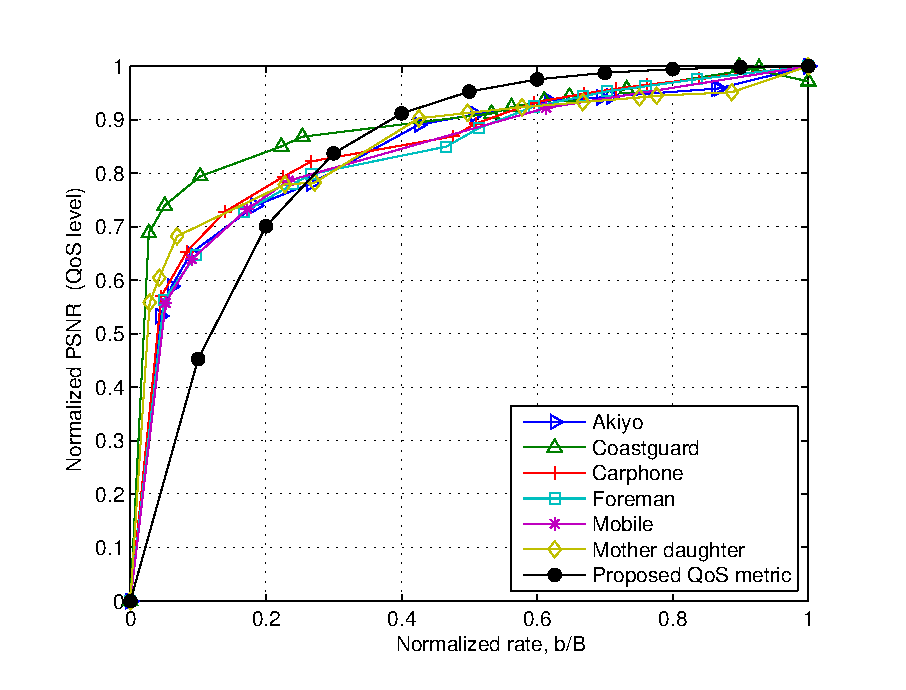
\includegraphics[width=0.75\textwidth] {cacop_qos_rate_cac.eps}
\end{center}
\caption{视频连接PSNR与码率的关系} 
\label{fig:chap_cacop:qos_rate_cac}
\end{figure}

\item 其它类型业务与QoS评价:
对于BE类型的业务,网页浏览HTTP应用或文件传输FTP应用是典型的例子。
HTTP(Hypertext Transfer Protocol)是互联网数据传输中最重要的应用层协议之一\cite{Fielding_1999}。 
由于其简捷、快速的方式特点,适用于分布式超媒体信息系统。
FTP是用于在网络上进行文件传输的一套标准协议。它属于网络协议组的应用层。用于Internet上的控制文件的双向传输。
同时,它也是一个应用程序(Application)。用户可以通过它把自己的PC机与世界各地所有运行FTP协议的服务器相连,访问和下载服务器上的大量程序和信息 \cite{Postel_Reynolds_1985}。
这两类业务应用的共同点是对用户对服务质量的要求取决于在发送端发送数据的总量与接收端已接收数据量的多少。
所以,我们把这类应用的服务质量简单地定义为\eqref{eqn:chap_cacop:BE_metric} 。
%
\begin{equation}
\label{eqn:chap_cacop:BE_metric}
\alpha^{others} = \frac{b}{B}
\end{equation}
%
其中,~$b$~是分配得到的带宽资源,~$B$~是对于BE类应用而言所需的带宽资源。
它们的比值就可以表示这类应用连接的服务质量水平。
对于最后两类业务nrtPS与ertPS,我们假定他们的业务与BE的类型类似,也用 \eqref{eqn:chap_cacop:BE_metric} 表示。
\end{enumerate}

综上所述,因为各类业务的服务质量的计算公式差别不大,下面我们将它们总结一下。
我们注意到\eqref{eqn:chap_cacop:qos_level_users}在业务特征值~$\rho$~趋向于$0$时存在极限,
且恰好是BE业务的服务质量计算公式。
%
\begin{equation}
\label{eqn:BE_limit}
\lim\limits_{\rho \to 0 } \frac{1- e^{-\rho \frac{b}{B} }}{1-e^{-\rho}} = \frac{b}{B}
\end{equation}

所以我们将\eqref{eqn:chap_cacop:BE_metric}改写为\eqref{eqn:chap_cacop:BE_metric_2}
%
\begin{equation}
\label{eqn:chap_cacop:BE_metric_2}
\alpha^{others} = \frac{b}{B} = \frac{1- e^{-\rho \frac{b}{B} }}{1-e^{-\rho}} \quad \text{if} \quad \rho \to 0
\end{equation}
%
最后我们将各种业务类型的服务质量评估公式整理可得\eqref{eqn:chap_cacop:alltype_metric}
%
\begin{equation}
\alpha = 
\begin{cases}
\delta_{b}(B), &\text{for UGS} \\
\frac{1- e^{-\rho \frac{b}{B} }}{1-e^{-\rho}}, \rho > 0& \text{for rtPS }\\
\frac{1- e^{-\rho \frac{b}{B} }}{1-e^{-\rho}}, \rho>0, \rho \to 0, &\text{for BE, nrtPS}\\
\end{cases}
\label{eqn:chap_cacop:alltype_metric}
\end{equation}
\section{资源分配的优化分析}
接纳控制的本质是为了保证各个连接的通信服务质量,防止新连接占用资源后对在线连接产生负面的影响。
一个好的接纳控制方法应该在充分利用资源的前提下,使用户的服务质量最大化。
这个问题可归结为如下的一个优化问题。
假设在系统中有~$M$~个 UGS连接,~$N$~个 rtPS 连接和 ~$Q$~个其它类型的连接,而且,这些连接之间是彼此无关的。
那么所有连接的QoS之和可以表示为基站的效用,如\eqref{eqn:chap_cacop:bs_qos} 所示。
\begin{align}
U_{BS} &= \displaystyle \sum_{i=1}^K \alpha_i \nonumber \\
&= \sum_{i=1}^M\alpha_i^{UGS} + \sum_{i=1}^N\alpha_i^{rtPS} + \sum_{i=1}^Q\alpha_i^{others} \nonumber \\
&=\displaystyle M^\prime + \sum_{i=1}^N \left( \frac{1- e^{-\rho_i^r
\frac{b_i}{B_i} }}{1-e^{-\rho_i^r}} \right)
 + \sum_{i=1}^Q \left( \frac{1- e^{-\rho_i^o
\frac{b_i}{B_i} }}{1-e^{-\rho_i^o}} \right),
\label{eqn:chap_cacop:bs_qos}
\end{align}
其中,~$M^\prime(\le M)$~ 表示~$M^\prime$~ UGS连接分配到了所需的带宽资源。
~$\rho_i^r$~ 是第~$i$~个rtPS连接的数据流特征。 
~$\rho_i^o$~ 表示BE类型的连接特征。此处我们假定这个很小且接近于零。
为了表示方便,我们用符号~$\rho_i$~来统一表示~$\rho_i^r$~ 和~$\rho_i^o$~。
~$U_{BS}$~ 表示基站在给~$K$~个连接提供服务所能收获的效用。
如果~$U_{BS}$~有最大值, 那么一定存在一个资源分配的优化解
~$\mathbf{b}$~ 。
我们会把这个解做为接纳控制的判决条件。
因此,这个优化问题可定义为如下形式。
\begin{align}
\mathbf{b}^* &= \arg \max \left\{ U_{BS}(\mathbf{b}) \big| \mathbf{b} = [b_1, b_2, \dots, b_K] \right\} \label{eqn_u_bs_qos}\\
&\text{subject to:}\nonumber\\
&\displaystyle\sum_{i=1}^{K}b_i + B_{ava}= B_{total} \nonumber
\end{align}
其中, ~$\mathbf{b}^*$~ 是资源分配的优化解。
~$B_{total}$~ 是系统所能提供的全部带宽。
~$ B_{ava} $~是剩余的带宽资源。

因为接纳控制通常是在业务负载大的情况下产生作用,所以为了简单起见,
我们剩余资源为零。同时,因为UGS类型的连接对带宽的要求严格,所以这些连接必须按照申请的数量分配。
我们则将上面的优化问题改写为 \eqref{eqn:chap_cacop:final_opt_qos}
\begin{align}{}
\label{eqn:chap_cacop:final_opt_qos}
\mathbf{b}^* &= \arg \max \left\{ U_{BS}(\mathbf{b}) \big| \mathbf{b} = [B_1, B_2, \dots,B_M,\right.
 \left. b_{M+1}, \ldots, b_K] \right\} \\
&\text{subject to:}\notag \\
&\sum_{i=1}^M B_i + \sum_{i=M+1}^{K}b_i= B_{total} \notag
\end{align}

下面我们来解这个优化问题。
先说明这个优化问题存在解。
为了方便书写,引入一个新的变量~$x$~来表示~$\frac{b}{B}$~。
\begin{equation*}
\begin{split}
x_i = \frac{b_i}{B_i} , i \in [M+1, K].
\end{split}
\end{equation*}
我们引入拉格朗日乘子~$\lambda$~,然后写出所需的拉格朗日方程,如
\eqref{eqn:chap_cacop:lagrange_defination}.
%%%
\begin{align}
&\displaystyle F(x_{M+1}, x_{M+2}, \dots, x_K, \lambda)= \sum^{M+N}_{i=M+1}
\left( \frac{1-e^{-\rho_i x_i}}{1-e^{-\rho_i}} \right) \nonumber \\
& \qquad \displaystyle +\sum_{i=M+N+1}^K\left( \frac{1-e^{-\rho_i x_i}}{1-e^{-\rho_i}} \right) 
 + \lambda
\left(B_{total} - \sum_{i=1}^M B_i -\sum^K_{i=M+1} x_i B_i \right).
\label{eqn:chap_cacop:lagrange_defination}
\end{align}
%%%
而后,对上面方程求两阶导数~$\frac{\partial ^2F}{\partial x_i \partial x_j}$~得Hermitian矩阵~${M}$~.
%%%
\begin{eqnarray*}
{M} = & 
\left[
\begin{array}{cccc}
\frac{\partial ^2F}{\partial x_{M+1} ^2} &\frac{\partial ^2F}{\partial x_{M+1} \partial x_{M+2}} & \dotsi & \frac{\partial ^2F}{\partial x_{M+1} \partial x_K} \\
\frac{\partial ^2F}{\partial x_{M+2} \partial x_{M+1}}& \frac{\partial ^2F}{\partial x_{M+2} ^2}& \dotsi & \frac{\partial ^2F}{\partial x_{M+2} \partial x_K}\\
\vdots & \vdots & \ddots & \vdots \\

\frac{\partial ^2F}{\partial x_{K} \partial x_{M+1} } &\frac{\partial ^2F}{\partial x_{K} \partial x_{M+2}} & \dotsi&\frac{\partial ^2F}{\partial x_K ^2}\\
\end{array}
\right] \\
=&
\left[
\begin{array}{cccc}
\frac{-\rho_{M+1}^2 e^{-\rho_{M+1} x_{M+1}}}{(1-e^{-\rho_{M+1}})} & & & \text{{\huge{0}}}\\
&&\ddots\\
\text{{\huge{0}}} &&& \frac{-\rho_{K}^2 e^{-\rho_{K} x_{K}}}{(1-e^{-\rho_{K}})}\\
\end{array}
\right] 
\end{eqnarray*}
很明显,如果~$\rho >0$~ 那么~$1-e^{-\rho} >0$~。
矩阵~${M}$~是负定的(negative-definite)。
因此对于BS的效用~$U_{BS}$~来说,存在局部极大值点。
下面我们来具体求解这个问题。
首先让对方程两连求一阶导数,并置为零,
~$dF = 0$~,则有下面一系列等式。
%%%
\begin{subequations}
\label{eqn_derivate}
\begin{align} &\frac{\partial F}{\partial x_{M+1}} =
\frac{\rho_{M+1} e^{-\rho_{M+1} x_{M+1}}}{(1-e^{-\rho_{M+1}})} - \lambda B_{M+1} = 0 \tag{\theequation -M+1}\\
&\frac{\partial F}{\partial x_{M+2}} =
\frac{\rho_{M+2} e^{-\rho_{M+2} x_{M+2}}}{(1-e^{-\rho_{M+2}})} - \lambda B_{M+2} = 0 \tag{\theequation -M+2}\\
\nonumber & \qquad \vdots \qquad \vdots \qquad \vdots \\
&\frac{\partial F}{\partial x_K} =
\frac{\rho_K e^{-\rho_K x_K}}{(1-e^{-\rho_K})} - \lambda B_K = 0 \tag{\theequation -K}\\
&\frac{\partial F}{\partial \lambda} = B_{total} - \sum_{i=1}^M B_i -
\sum^K_{i=1}x_iB_i = 0 \tag{\theequation -K+1}
\end{align}
\end{subequations}
%%%
根据公式 (\ref{eqn_derivate}),我们有
%%%
\begin{equation*}
\begin{split}
&\frac{\partial F}{\partial x_i} = \frac{\rho_i e^{-\rho_i
x_i}}{(1-e^{-\rho_i})} - \lambda B_i = 0\\
%\implies &\rho_i e^{-\rho_i x_i} =\lambda B_i(1-e^{-\rho_i})\\
%\implies &\ln\rho - \rho x_i = \ln [\lambda B_i (1-e^{-\rho_i})]\\
\implies &x_i = \frac{1}{\rho_i} \ln \left[ \frac{\rho_i}{\lambda B_i(1-e^{-\rho_i})} \right] \\
\end{split}
\end{equation*}
%%

再将 ~$x_i$~ 代入公式 (\ref{eqn_derivate}-K+1),则又有
%%%
%
\begin{equation}
\begin{split}
&B_{total} -\sum_{i=1}^MB_i = \sum_{i=M+1}^K x_i B_i \\
&= \sum_{i=M+1}^K \frac{B_i}{\rho_i} \ln \left[ \frac{\rho_i}{\lambda B_i(1-e^{-\rho_i})} \right] \\
%&= \sum^K_{i={M+1}}\left[- \frac{1}{\rho_i}\ln \lambda - \frac{1}{\rho_i}
%\ln (B_i) - \frac{1}{\rho_i} \ln (1-e^{-\rho_i}) + \frac{1}{\rho_i}
%\ln
%\rho_i \right] B_i\\
%&= \sum^K_{i={M+1}}\left[- \frac{B_i}{\rho_i} \ln \lambda -
%\frac{B_i}{\rho_i} \ln (B_i) - \frac{B_i}{\rho_i} \ln (1-e^{-\rho_i})
%+ \frac{B_i}{\rho_i} \ln
%\rho_i \right]\\
%&= -{\ln \lambda}\sum^K_{i={M+1}} \frac{B_i}{\rho_i} 
%- \sum^K_{i={M+1}} \frac{B_i \ln (B_i)}{\rho_i} 
%- \sum_{i={M+1}}^K \frac{B_i\ln(1-e^{-\rho_i})}{\rho_i} \\ 
%& \hspace{5mm}+ \sum^K_{i={M+1}} \frac{ B_i\ln \rho_i} {\rho_i} \\
\end{split}
\label{eqn_find_mu}
\end{equation}

%%%
基于公式 (\ref{eqn_find_mu}), 我们可以解出~$\lambda$~.
%%%
\begin{equation*}
\begin{split}
\lambda &= \exp \left( \frac{\sum_{i=M+1}^K \frac{B_i}{\rho_i} \ln \left[ \frac{\rho_i}{B_i(1-e^{-\rho_i})} \right]
}{\sum_{i=M+1}^K \frac{B_i}{\rho_i}} \right.
+ \left. \frac{ 
\sum_{i=1}^M B_i - B_{total}}{\sum_{i=M+1}^K \frac{B_i}{\rho_i}} \right)\\
\end{split}
\end{equation*}
%%%

然后,可以求得
%%%
%
\begin{equation}
\begin{split}
x_i & = \frac{1}{\rho_i} \ln \frac{\rho_i}{B_i(1-e^{-\rho_i})} \\
&-\frac{1}{\rho_i}\left( \frac{\sum_{j=M+1}^K \frac{B_j}{\rho_j} \ln \left[\frac{\rho_j}{B_j(1-e^{-\rho_j})}\right] 
}{\sum_{j=M+1}^K \frac{B_j}{\rho_j}} \right)
-\frac{1}{\rho_i}\left( \frac{ 
\sum_{j=1}^M B_j - B_{total}}{\sum_{j=M+1}^K \frac{B_j}{\rho_i}} \right) \\
\end{split}
\end{equation}
%
%%%

最后,整理可得带宽分配的解。
%
\begin{equation}
\begin{split}
\mathbf{b^*}& = [b^*_{M+1}, \cdots, b^*_{K}]\\
b_i^* & = x_iB_i = \frac{B_i}{\rho_i} \ln \frac{\rho_i}{B_i(1-e^{-\rho_i})} \\
&-\frac{B_i}{\rho_i}\left( \frac{\sum_{j=M+1}^K \frac{B_j}{\rho_j} \ln \left[\frac{\rho_j}{B_j(1-e^{-\rho_j})}\right] 
}{\sum_{j=M+1}^K \frac{B_j}{\rho_j}} \right)
 -\frac{B_i}{\rho_j}\left( \frac{ 
\sum_{j=1}^M B_j - B_{total}}{\sum_{j=M+1}^K \frac{B_j}{\rho_i}} \right), i \in [M+1, \cdots, K] \\
\end{split}
\label{eqn:chap_cacop:b_i_bw}
\end{equation}
%
\section{提出的接纳控制算法}
\label{sec_alg}


基于上一节所得到的带宽分配方案,我们提出一个接纳控制算法。
在此算法中,我们假设分配到资源数量应该大于业务所需的最小数量,即
~$b_i^* \ge B_i^{\min}$~. 
这个最小值与业务的类型相关。不同业务均有所不同。
例如,对于话音应用来说,它所需的带宽的最小值就被设置为它申请值。
对于象视频这样的rtPS应用,一般~$b_i>=B_i^{\min}$~
对于新用户~$K$~而言,
如果~$b_K^*$~ 小于所需的资源的最小值~$B_K^{\min}$~,系统会拒绝这个连接进入。
因为如果按这样的资源量分配给连接~$K$~,服务质量会很差,用户肯定不满意。
另外,
在我们的算法,使用了优级的概念。我们假定在线连接的优先级要比新连接的优先级要高。这样的假定会造成在我们的算法中在线用户的通信不会被系统中断。


\begin{algorithm}[H]
\SetAlgoLined
% assume ~$B_{ava}=0$~\;
等待一个新的连接进入请求\;
新连接~$K$~申请进入;假定此时系统中有~$K-1$~连接正在进行通\;
\eIf {~$B_K<= B_{ava}$~}{
允许连接~$K$~进入系统,被分配带宽~$B_K$~\;
}{
根据资源分配\eqref{eqn:chap_cacop:b_i_bw}计算~$\bf b^*$~\;
\If{~$b_i^* < B_i^{\min} $~}{
连接~$i$~被系统列入本次的保护范围,且
~$B_{total} = B_{total} - b_i^{old}$~
, ~$K = K-1$~ \;
{\bf{go to 6}}\;
}
\eIf{~$b_K< B_K^{min}$~}{
拒绝新连接的请求\;
{\bf{go to 1}}\;
}{
允许新连接~$K$~进入系统\;
\For{~$i=1$~ \KwTo ~$K-1$~}{
被保护的连接保持原有的资源不变\;
对于其它的连接按计算的优化资源分配方案~$b_i$~执行\;
}
分配资源~$b_K^*$~ 给新连接~$K$~\;
}
}
{\bf{go to 1}}\;
\caption{提出的接纳控制算法} \label{alg:chap_cacop:agr_cac}
\end{algorithm}


由于上述的两个假定,我们的算法会在带宽分配的过程中出现迭代。
比如,如果一个在线的连接由资源分配 \eqref{eqn:chap_cacop:b_i_bw}计算所得的资源数目小于它的最小资源需求数目,我们认为这个连接应该受到保护。
接纳算法会将取消此次计算过程,将此连接和它占用的资源排除在外,
然后再重新启动新一轮的带宽计算过程。
直到不再出现在线连接所分配的资源会小于它最低要求。
对于连接~$K$~来说,如果最后的结果大于其最低要求,则允许其进入系统;否则,这个连接会被系统阻塞(blocked)。


当一个新连接提出进入系统的申请时,接纳控制单元启动判断过程。
如果当前的空闲资源大于新连接~$K$~所需的资源数量,
那么新连接会被允许进入系统接受服务,并分配给资源~$B_K$~。
否则,系统进入优化资源分配的计算过程。
在一个空闲资源缺乏的情况下,一个新连接被系统接纳需要满足两个条件:
一是对于新连接~$K$~来说,优化的资源分配值~$b_K$~要大于最低资源需求~$b_K^{\min}$~。
另一个是对于其它在线的连接所分配到是优化资源值~$b_i$~也要大于各自的最低资源需求。
因此这个算法会尽可能将基站系统的效用保持较高的水平。
算法的详细流程如流程{\bf{算法 \ref{alg:chap_cacop:agr_cac}}}所示。
其中,步骤7、8、9用来将那些需求保护的连接排除出分配方案中。
%%算法描述


\section{仿真实验与分析}
\begin{figure*}[tb]
\centering
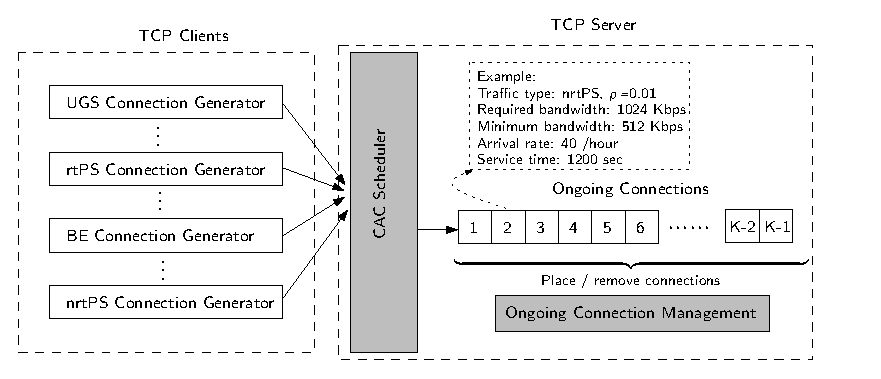
\includegraphics {cacop_simulator.eps}
\caption{系统仿真模型} 
\label{fig:chap_cacop:sim_cfg}
\end{figure*}
我们通过构造一个系统的仿真模型来评估所提出的算法。
这个仿真的模型如\figref{fig:chap_cacop:sim_cfg} 所示。
为了能够去除一些仿真中的随机因素,仿真脚本被运行多次来得到一个统计意义的结果。

\subsection{仿真模型}
我们根据本章第三小节介绍呼叫接纳控制模型,建立了这样一个仿真模型。
模型包括下面几个组成部分:
\begin{itemize}
\item 伪连接产生单元(Pseudo Connection Generators): 它能够按照泊松分布产生新的连接,就象在排队论中“顾客”。
    时间间隔~$T$~来自于一个指数分布,如\eqref{eqn:chap_cacop:exp_model}定义。
%
\begin{equation}
\label{eqn:chap_cacop:exp_model}
F_T(t) = 1 - P_0(t) = 1 - e^{-\lambda t}
\end{equation}
%
\begin{table}[tb]
\caption{连接的业务类型} \label{tb:chap_cacop:sim_cfg}
\begin{center}
\begin{tabular}{cccccc}
\toprule
业务类型 &~$\rho$~ &所需的 & 最小的 &到达 &接受服务时间 \\
Type & &bandwidth & bandwidth & rate & time \\
&&(Kbps)& (Kbps) & (/hour) &(seconds) \\
\midrule
UGS& N/A &64 &64 & 100 &600\\
BE & 0.01&90 &64 &90 &700\\
rtPS &4& 128 &64 &80 &800\\
rtPS &5& 256 &128 &70 &900\\
BE &0.01& 384 &192 &60 &1000\\
nrtPS &0.01& 768 &384 &50 &1100\\
nrtPS &0.01& 1024 &512 &40 &1200\\
rtPS &6& 1512 &756 &40 &1200\\
rtPS &7& 1768 &884 &30 &1500\\
rtPS &8& 2048 &1024 &30 &1500\\
\bottomrule
\end{tabular}
\end{center}
\end{table}
到达率根据不同业务类型及应用假设为每小时 ~$30 \text{ to } 100 $~。
每个连接都设置有最小带宽需求与业务类型特征值。
带宽需求数量在64Kbps到2Mbps之间。
并且,假设接受服务的时间为一个均值为600到1500秒指数分布的随机变量。
表\ref{tb:chap_cacop:sim_cfg}详细地列出其中的各项参数。

\item 在线连接管理单元(Ongoing Connection Management): 当一个连接被系统接入后,会放入一个队列中进行管理。当它的服务时间结束时,管理单元会将它从队列中删除。

\item 呼叫接纳控制单元(Call Admission Control Scheduler): 此单元负责计算每一个连接应分配的资源数量,并分配总共~$B_{total}=75Mbps$~的带宽资源。 
\end{itemize}
作为对比算法,我们使用了两种常见的方法。
第一个标记为“Baseline”。这种方法在进行接纳判断时,只是根据剩余的空闲带宽能否满足新连接的要求。
如果空闲带宽足够,则接入;否则,则拒绝进入。
另外一种是由学者EL Kadi提出的资源保留算法。该算法在系统的总资源中保留一定比例专门针对新连接的接入\cite{EL-Kadi2002}。
%%%%%
\subsection{仿真结果}
%
\begin{table}[htbp]
\caption{仿真结果汇总} \label{tb:chap_cacop:res_sim}
\begin{center}
\begin{tabular}{lrrr}
\toprule
&Baseline &Elkadi &Proposed\\
\midrule
阻塞率 (\%) &4.15 & 0 &0.82\\
资源利用率(\%) &86.70 &83.57 &88.42\\
系统连接容量 &137.55 &145.60 &144.01\\
连接的平均QoS &1.00 &0.94 &0.98\\
基站系统的效用 &137.55 &136.28 &141.19\\
\bottomrule
\end{tabular}
\end{center}
\end{table}
表 \ref{tb:chap_cacop:res_sim} 汇总了三种方法的仿真结果。
我们在仿真过程中,不但考察了传统的性能指标,如新连接的阻塞率,资源利用率以及系统连接容量,而且还评估了本章所提出的QoS的测量值,以及基站系统的整体效用。
在三种方法中,本文所提出的算法在资源利用率及系统效用方面性能表现最好,
资源利用率分别比其它高出~$2\%$~和~$4\%$~;系统整体效用值比其它两个方法高约4和5。
在阻塞率真这一项,所提出的方法与基准方法“Baseline”相比较,阻塞率下降了五倍,从~$4.15\%$~ 降至为 ~$0.82\%$~。
因为在ELKadi的资源预留方法中,资源对新连接总是优先使用的,所以这种方法会将新连接的阻塞率降为零。而所提出的方法为~$0.82\%$~,与ELKadi方法十分接近。
从各项指标的整体来看,我们所提出的方法综合的性能较优。
%The baseline method maximizes the average QoS level of the ongoing connections, because it must block new connections in the heavy traffic load condition. 
%%%%%%%
%
\begin{figure}[htbp]
\centering
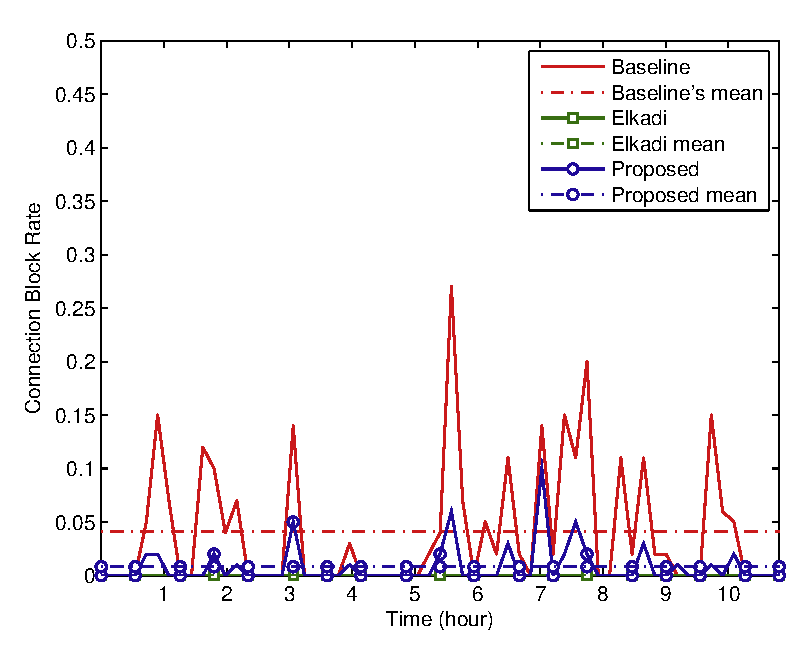
\includegraphics[width=0.65\textwidth] {cacop_block_rate.eps}
\caption{新连接的阻塞} \label{fig:chap_cacop:clock_accept_block_drop}
\end{figure}

%%%%%%%
%
\begin{figure}[htbp]
\centering
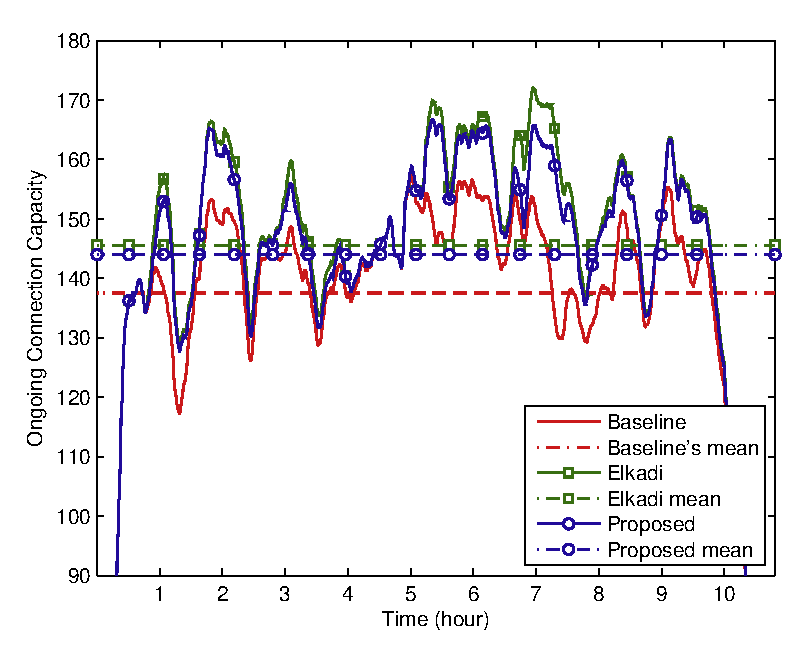
\includegraphics[width=0.65\textwidth] {cacop_conns_sum.eps}
\caption{系统的连接容量}\label{fig:chap_cacop:clock_onging_call_sum}
\end{figure}

%%%%%%%
% 
\begin{figure}[htbp]
\centering
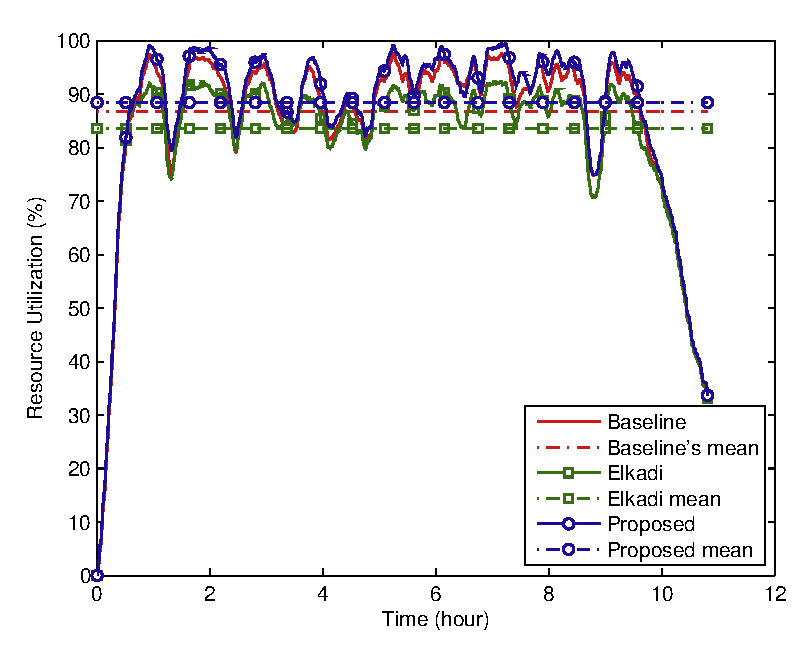
\includegraphics[width=0.65\textwidth]{cacop_bw_utilization.eps}
\caption{系统资源利用率}\label{fig:chap_cacop:clock_bs_availble_bw}
\end{figure}

%%%%%%%
%
\begin{figure}[htbp]
\centering
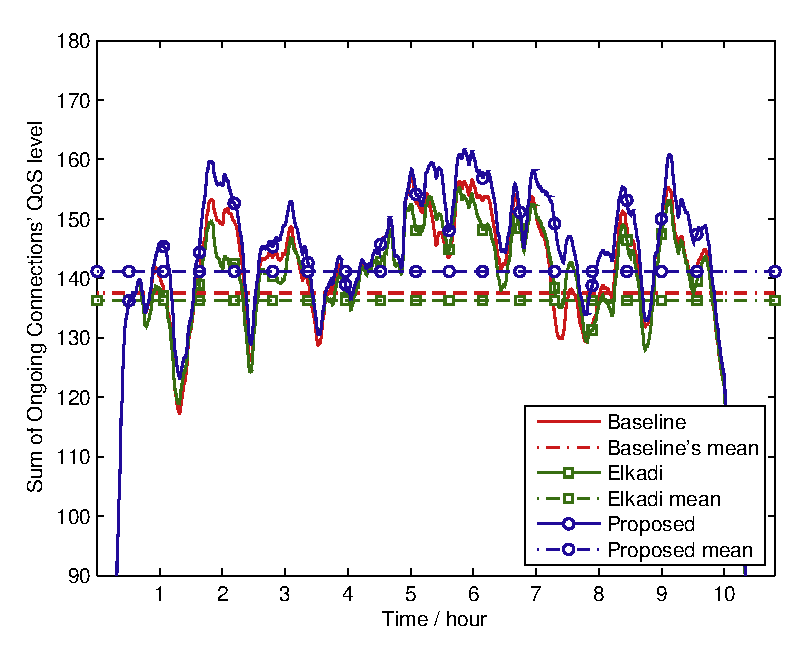
\includegraphics[width=0.65\textwidth] {cacop_qos_sum.eps}
\caption{基站系统整个效用}\label{fig:chap_cacop:clock_bs_qos_sum}
\end{figure}

%%%%%%%
% 
\begin{figure}[htbp]
\centering
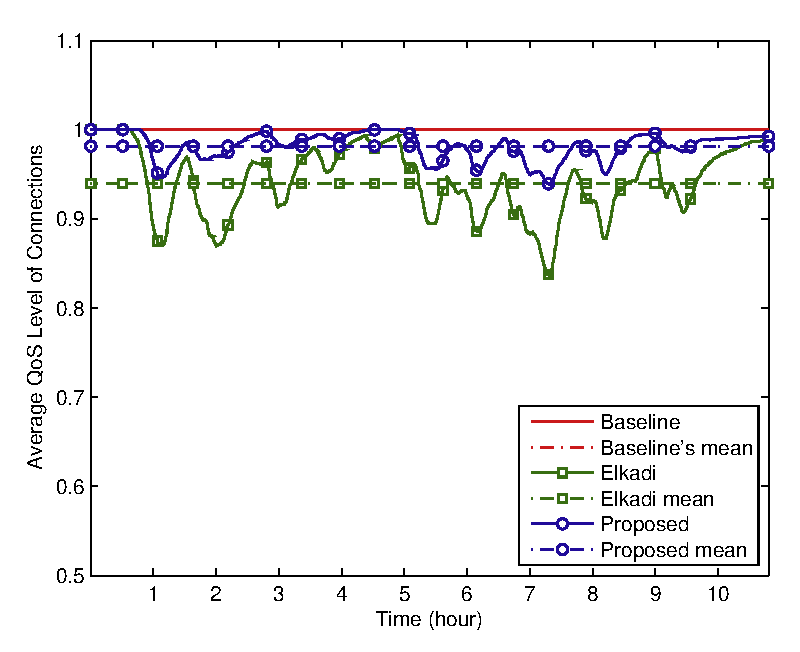
\includegraphics[width=0.65\textwidth] {cacop_avg_qos.eps}
\caption{连接平均QoS水平}\label{fig:chap_cacop:clock_avg_call_qos}
\end{figure}


%On contrast, the proposed method can increase by up to 6 \% bandwidth utilization by making the slight degradation of block rate. The performance of the QoS level of BS can achieve the best one among them to 141.4 while the average QoS level of connections is kept as 0.984, just to decrease by 0.16 in comparison with maximum value, one. 

另一方面,\figref{fig:chap_cacop:clock_accept_block_drop} 到 \figref{fig:chap_cacop:clock_avg_call_qos} 显示了各个指标在整个仿真过程中实时的情况。
这里的每一幅图中我们绘制了六条线。其中,水平的虚线是各个算法的均值。

如\figref{fig:chap_cacop:clock_accept_block_drop}所示,新连接的阻塞率在整个仿真的过程中均保持着很低的水平。
同时,还可清楚的看到“Baseline”算法的阻塞率的值波动较大。
\figref{fig:chap_cacop:clock_onging_call_sum} 显示了在线连接的容量数目,可以看出,ElKadi方法与本文所提算法曲线非常接近,且明显优于基准算法。
对于资源利用率,与其它二个算法相比较,ElKadi的性能最差。这也可以看出,预留算法的缺陷。由于在高业务负载下,预留算法为了保证新连接能够及时的接入,使得一部分的资源未得到充分地利用,如 \figref{fig:chap_cacop:clock_bs_availble_bw}所示。
 
从用户的角度看,QoS水平曲线对于单个用户更有意义一些。
如\figref{fig:chap_cacop:avg_qos}所示,
这些曲线表示的是在线用户的QoS水平和满意度。,我们所提出的方法明显优于ElKadi的算法。同时,我们还可看出,基准算法的平均QoS水平总是最高的,始终维持在常量最大值~$1$~。基准算法通过牺牲新连接服务质量使得在线用户服务质量得到了最大程度的保证。
从这些仿真结果,我们清楚地看到,在一个资源受限的系统中,系统性能指标之间是存在矛盾的。通常将其中一个性能指标得到改善和提高的同时,会使得另外一个性能指标下降。譬如在线用户的QoS水平与新用户的阻塞率。从仿真的结果来看,我们所提出的算法在平衡相互矛盾的系统指标方面,比其它两种方法要好。我们的算法兼顾了新用户与在线用户的利益,并进行了很好的平衡与折衷。

\section{小结}
本章研究的是基于多媒体业务下的呼叫接纳控制问题。
首先我们通过分析不同的多媒体业务特点,
建立一个针对网络底层资源分配参数与网络高层的业务QoS水平的映射机制,
实现不同业务用户的QoS测度以及系统整体性能的有效测量。
并且,基于这个映射模型,提出了一个基于在线用户和与新用户利益兼顾呼叫接纳控制与资源分配的优化算法,
实现不同业务Qos以及系统资源的在线管理。
该算法以用户服务质量效用为最大化目标,在高负荷下依据用户业务负载情况调整接纳与分配策略,达到各项性能指标的一个较好平衡也折衷。
%
%%
%%



%
\graphicspath{ {../body/nash_bargaining_figures/} }
\chapter{基于议价博弈的多用户资源分配策略}
\echapter{Bargaining Game on Resource Allocation for Multiple Users}
%\label{chap_nash_bargain}
在带宽资源受限的无线网络中,多个用户对资源的需求存在着天然的竞争性。
同时,不同用户的多媒体应用,诸如视频播放、在线游戏或网页浏览等,也都十分常见。
为了能够保证每个用户业务的正常进行,系统资源分配的算法需求照顾到系统中每个应用的不同服务质量要求。
博弈论作为在经济学中已经普遍使用的一门数学理论,近年来也被引入到无线通信领域,特别是用来解决无线资源管理的问题。
在本章中,我们提出了基于议价的合作博弈模型来描述系统中用户之间的竞争状况。通过对这个模型的求解,
可以公平地把系统资源分配给网络中的每个用户。
所得到的纳什议价解是一个公平且优化的资源分配解决方案。
这个方案既可以使系统资源充分利用,又能保证每个用户资源分配的公平性。

\section{引言}
\esection{Introduction}
博弈论除了在利益相互冲突与矛盾的状况下寻找解决问题的方法,也寻求在合作的框架下解决问题的方案。
议价博弈理论就是合作博弈论的一个理论分枝。
它最初提出的原因是为了要解决在经济活动中,双边垄断市场结构下的价格决定问题。
例如,对于日常生活中的房屋买卖问题。
参加博弈的一方是卖房者,另一方是买房者。
双方都基于一个共同的利益基础,希望以一个合适的价格来完成房屋产权的转移。
然而,在这个讨价还价的过程中存在着一个潜在的冲突和矛盾:当卖房者期望一个高的卖出价格的同时,买房者却期望一个低的买入价格。
与此同时,双方也都不想失去可能因合作而获得的收益机会,
那么,他们一定会寻找一个方法来解决这个矛盾。
在传统的经济学供给需求分析框架中,我们不能确切地知道最终的均衡价格到底在什么位置。
传统的经济学理论只是模糊地说,均衡价格取决于博弈双方的谈判能力,也就是所谓的“议价能力”。
但是议价能力的具体描述取决于一些比较模糊的因素,例如双方的谈判次数、市场对谈判的期望等等。
而议价博弈理论的出现,使得人们可以用数理的方式解决这些类似的问题。

议价理论在博弈理论的研究中十分重要,它更加完善地考虑到了个人理性与集体理性的问题。

\begin{itemize}
\item 个人理性:对于博弈双方而言,
双方在议价解下所得的效用要必须高于双方不进行博弈或放弃博弈所得的效用。
也就是说博弈者为了得到更高的收益而主动地进行议价博弈。
\item 集体理性:议价的最终结果应该具有帕累托(Pareto)最优性质。
在达到最终的议价结果时,任何一方都不可能在不损害对方利益的情况下增加自己的收益。
\end{itemize}

例如,如\figref{fig:chap_bargain:bargain_basic_concept}所示。
其中,~$u_1$~与~$u_2$~表示议价双方各自的收益。
集合~$\phi$~是所有可能出现的效用向量~$\mathbf{u}=(u_1,u_2)$~的集合。
~$\mathbf{d}=(u_1^d, u_2^d)$~表示博弈双方提前约定如果不能达成合作协议时,最终双方取得的效用向量。
扇形区域~$BdC$~表示所有符合个人理性的效用向量集合,而集合的边界弧线ABCD表示符合集体理性的效用向量集合。
两者的交集弧BC是可能的议价区域,包括了所有可能达到的议价解。
不难理解,BC弧上所有的点都具有帕累托最优的性质。
但是最终的议价解将出现在什么位置就不得而知。
如果想获得唯一的议价解,就需要对上述议价问题附加一些其他的条件。
接下来,我们先建立一个资源竞争的议价博弈模型,然后再讨论这些附加的条件。
\begin{figure}[!tb] 
    \centering
   \begin{minipage}[t]{0.65\linewidth} 
    \centering 
    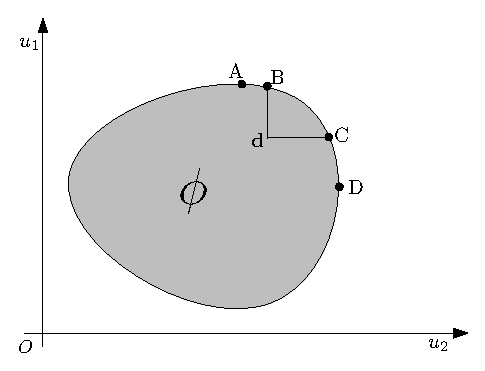
\includegraphics[width = \textwidth]{bargain_basic_concept} 
    \caption{两用户议价概念示意图} 
    \label{fig:chap_bargain:bargain_basic_concept} 
  \end{minipage}%
\end{figure}


\section{资源分配博弈模型}
\esection{Game Model of Resource Allocation}
\subsection{议价博弈建模}
\esubsection{Modelling the Bargaining Game}
假设在一个资源受限的无线网络系统中,存在有~$n$~个用户。
他们以合作的方式或“议价”的方式来分配网络所提供的带宽资源。
每一个用户都有自己的效用函数~$U_i(b_i)$~。
效用函数由它当前分配到的带宽~$b_i$~、期望申请到的带宽~$B_i^{req}$~和一个最低效用~$U_i(b_{0i})$~决定。
这里,我们假设最低效用被定义为分歧点(Disagreement Point), ~$d$~。 
分歧点的设置是用户之间为了防止最终没能达成合作协议时预先确定的的效用收益。
令~$\phi = \{ \mathbf{U} \} \subset R^n$~为效用的集合。
其中,~$\mathbf{U} =( u_1 =U_1(b_1), \ldots, u_n = U_n(b_n))$~。
令~$\mathbf{d} = (d_1, \ldots, d_n)$~是用户的分歧点。
其中,~$d_i = U_i(b_{0i})$~。
所以,此博弈问题定义为 ~$(\mathbf{\phi,d})$~。
接下来我们来描述此博弈的细节。

首先定义博弈参与者的效用。
在第 \ref{chap_cacop} 章(呼叫接纳控制算法)中,我们曾经定义过服务质量水平。
此处我们仍旧延用指数函数归一化形式来定义用户连接的QoS水平,如\eqref{eqn:chap_nash:qos_definition} 所示。
\begin{equation}
QoS = \frac{1- e^{-\rho \frac{b}{B} }}{1-e^{-\rho}}, \rho > 0
\label{eqn:chap_nash:qos_definition}
\end{equation}
其中,~$b$~ 表示博弈参与者最终分配到的资源数量。
~$B$~表示博弈者在提交申请时,希望能够分配到的资源数量。
~$\rho$~表示业务的特征值。

因为QoS的大小与~$\rho \frac{b}{B}$~紧密相关,
且\eqref{eqn:chap_nash:qos_definition}是单调增函数,
所以我们定义用户效用的简化计算公式,如 \eqref{eqn:chap_nash:utility_definition}所示。
\begin{align}
   u_i =  U_i(b_i) = \rho_i \frac{b_i}{B_i^{req}}
    \label{eqn:chap_nash:utility_definition}
\end{align}
其中,下标~$i$~是指系统中的第~$i$~个博弈参与者。
因为~$b_i\ge 0$~,且~$B_i^{req}$~和~$\rho$~都大于零,所以~$U_i(b_i)\ge0$~。
另一方面,由于系统的资源是有限的,所以要求满足约束条件,~$\sum_i^n b_i \le B_{total}$~
其中,~$B_{total}$~是系统所能提供的资源数量。
对于分歧点,我们假设每个博弈参与者有一个最低资源要求~$B_i^{\min}$~,
令~$B_{0i} = B_i^{\min} $~,~$d_i = \rho_i \frac{B_i^{\min}}{B_i}$~。
同时,也要求~$b_i$~大于$B_i^{\min}$~。

\subsection{议价博弈解的定义与分析}
\label{subsec:chap_nash:math_analysis}
\esubsection{Definition and Analysis of Bargainning Solution}

我们先定义议价博弈的数学形式,然后再分析它的解的情况。
博弈的解从数学上的表示,其实是一个映射函数,即,~$F: \mathbf{\phi} \rightarrow R^n$~,
记作~$F(\phi, \mathbf{d})$~。

符合帕累托最优的博弈解在效用集合的一部分边界上,这部分边界记作~$B$~,有时也称为议价集合。
~$\mathbf{s}$~表示这部分边界上的点,用 \eqref{eqn:chap_nash:points_bargain}表示。
\begin{align}
 \mathbf{s} = \sum_{i=1}^n \alpha_i \mathbf{r}_i
    \label{eqn:chap_nash:points_bargain}
\end{align}
其中,~$\alpha_i$~表示议价能力,且满足~$\sum_{i=1}^n \alpha_i = 1$~。
~$\mathbf{r}_i, i= 1,\dots,n$~是~$n$~维空间中一个点。~$\mathbf{s} = \alpha_i \mathbf{r}_i$~为多维空间的一个超平面。
如果与集合~$\phi$~只有一个交点,此平面也称为支撑平面(supporting plane),记为 ~$S$~。
如果以分歧点为起始点,画出~$n$~条与空间坐标轴平行的线,那么这些平行线与平面~$S$~的交点就是~$\mathbf{r}_i, i= 1,\dots,n$~。
所有满足上述条件的点的集合记作~$B$~,博弈论中称为可行集~$\mathbf{B}$。
例如在二维情况下,如\figref{fig:chap_bargain:2_dim_nash_bargain}所示。这个超平面退化为一条支撑线(supporting line),而这些点~$\mathbf{r}_i, i= 1,2$~就是与过分歧点与横轴平行的线、与纵轴平行的线的交点。

\begin{figure}[!tb] 
    \centering
   \begin{minipage}[t]{0.6\linewidth} 
    \centering 
    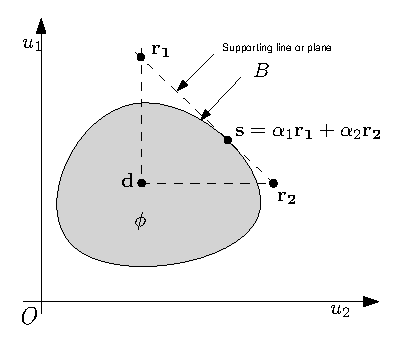
\includegraphics[width = \textwidth]{chap_nash_2_dim_nash_bargain.eps} 
    \caption{两用户议价解示意图} 
    \label{fig:chap_bargain:2_dim_nash_bargain} 
  \end{minipage}%
\end{figure}

综上所述,议价博弈的符合帕累托最优的解可以写为\eqref{eqn:chap_nash:game_solution},
\begin{align}
    F(\mathbf{\phi},\mathbf{d}) = \left\{ \mathbf{s} \in \mathbf{B} \big \vert \mathbf{s} = \sum_{i=1}^n \alpha_i \mathbf{r}_i \right\}
    \label{eqn:chap_nash:game_solution}
\end{align}
注意,点~$\mathbf{s}$~也是集合~$\phi$~边界上的点。

前面提到,在此情况下,符合帕累托最优的议价解不止一个。
经济学家纳什提出如果满足一些条件,
那么就可以确定一个唯一的、更合理的解\cite{Nash_1950}。

这些条件也称之为纳什公理约束。
这里,我们以两个参与者为例来解释一下这些约束的意义。
如果在一个议价博弈过程中存在有两个参与者。
他们在博弈中可以有多种的选择。
两者的选择会共同造成各自所得到的效用。
很明显,他们都会追求使自己的效用最大化的选择。
各自的效用分别记为~$u_1$~和~$u_2$~。
类似前面的定义,记号~$\phi$~表示效用向量~$\mathbf{u}=(u_1, u_2)$~的非空紧凸集合(Closed and bounded)。
并且,双方附加一个条件:如果博弈双方不能达成一个有约束力的协议的话,
那么,双方将会得到事先定好的效用~$\mathbf{d}=(d1, d2)$~。
效用向量~$\mathbf{d}$~也被称作“分歧点”(disagreement points)。
纳什议价博弈模型的解是这样一个函数~$f$~,该函数可以将集合~$\phi$~映射到解集上。
纳什提出以下具体的公理:

\begin{itemize}
\item 公理一:个体理性(Individual Rationality) 
    对于用户~$i$~而言, ~$u_i^* \ge d_i$~
\item 公理二:可行性(Feasibility),解满足关系式~$\mathbf{u}^* \in \phi$~
\item 公理三:弱帕累托最优性质(Weak Pareto Optimality)\\
如果~$\mathbf{u} \in \phi$~,而且~$\mathbf{u} \ge \mathbf{u}^*$~,那么可以推导得到 ~$\mathbf{u} = \mathbf{u}^*$~
\item 公理四:对称性(Symmetry),\\
如果~$d1=d2$~ 并且如果~$(u_1, u_2) \in \phi \Rightarrow (u_2, u_1) $~, 一定有 ~$u_1^*= u_2^*$~。
\item 公理五:线性变换无关( Independence of Linear Transformations)\\ 
如果~$\forall (a_1, a_2, b_1, b_2) \in R$~,如果我们定义函数~$g$~是将所有向量~$(u1, u2)$~映射到~$(u1', u2')$~的线性变换函数,例如~$u_i^\prime=a_iu_i+ b_i (i =1,2)$~,于是我们有 ~$f[g(\phi), g(d)]=g[f(\phi , d)]$~。
\item 公理六:无关选择的无关性(Independence of Irrelevant Alternatives) \\
如果集合~$\psi \subset \phi$~ ,
并且~$f(\phi,d) \in \psi$~,那么可得 ~$f(\psi,d) = f(\phi,d)$~ 。
\end{itemize}
其中,公理一、公理二和公理三定义了议价解集合~$B$~。
最终的纳什议价解(Nash Bargaining Solution,NBS)也在议价解集合中。
公理三保证了集体理性,对于博弈参与者而言,在议价可能集内不存在好于议价解的效用向量。
公理四、公理五和公理六称为公平性公理。
公理四描述了如果用户有相同的“分歧点”和效用函数,那么它们的效用一定相同。
比如,对称博弈中博弈双方有完全相同的策略可能性及相同的议价能力。
公理五表明如果效用变换函数如果是线性的,那么最终议价解是不变的。
公理六表明如果在一个集合的最终议价解在一个小的子集内找到,这个子集的解也就是这个集合的解。
也就是说,如果逐步从原来的可行集中排除一些无关选择,并不改变最终的议价解。
这条公理在议价的过程中可以解释为博弈双方会出现自愿地相互让步。
这些公理所描述的本质数学含义其实是:议价解仅仅依赖于~$\mathbf{u}^*$~邻域中可行集右上边界的形状。

如果一个博弈问题满足以上公理,
可以证明纳什议价的唯一解便是使纳什积最大化的效用向量\cite{Nash_1950},即
\begin{align}
\mathbf{u}^* = \arg \max \prod_i^n (u_i-d_i)
\label{eqn:chap_nash:nash_product}
\end{align}

\subsection{议价博弈模型求解}
\esubsection{Solution of Game Model}
由博弈的定义可看出,我们博弈模型首先可以满足公理一、二、四。
因为公理三、五和六所描述的内容,从数学定义上来讲要求效用集合是凸集。
所以,接下来我们证明根据\eqref{eqn:chap_nash:utility_definition}所定义的资源分配的效用向量集合~$\mathbf{\phi}$~是凸集(convex set)。

定理:如果效用向量集合~$\mathbf{\phi}$~中的元素如\eqref{eqn:chap_nash:utility_definition}所定义,那么这个集合是一个凸集。

证明:我们知道,如果一个集合~$\mathbf{\phi}$~是凸集,
那么对于这个集合中的任意两个元素,~$\mathbf{x}$~和~$\mathbf{y}$~,以及一个任意的数~$\theta$~, ~$0\le \theta\le 1$~来说,凸组合~$\mathbf{z}=\theta \mathbf{x} + (1-\theta) \mathbf{y}$~所构成的元素也属于集合~$\mathbf{\phi}$~。

我们用大写记号~$\mathbf{X}$~ 和~$\mathbf{Y}$~表示博弈效用集合中的任意两个元素,则有
\begin{align*}
    \mathbf{X} &=\left( (U(b_1), U(b_2), \ldots, U(b_n) \right)
    = \left( \rho_1 \frac{b_1}{B_1^{req}},\rho_2 \frac{b_2}{B_2^{req}},\ldots, \rho_n \frac{b_n}{B_n^{req}} \right) \in \mathbf{\phi} \\
    \mathbf{Y} &=\left( (U(b_1^\prime), U(b_2^\prime), \ldots, U(b_n\prime) \right)
    = \left( \rho_1 \frac{b_1^\prime}{B_1^{req}},\rho_2 \frac{b_2^\prime}{B_2^{req}},\ldots, \rho_n \frac{b_n^\prime}{B_n^{req}} \right) \in \mathbf{\phi} 
    %\label{eqn:chap_nash:two_elements}
\end{align*}
其中,~$(b_1, b_2, \ldots, b_n)$~和 ~$(b_1^\prime, b_2^\prime, \ldots, b_n^\prime)$~是分配的资源数量,且满足~$b_i \ge 0$~ ,~$b_i^\prime \ge 0$~, ~$i = 1, \ldots, n$~。

那么,可以推导出 $b_i$ 和 $ b_i^\prime$,
\begin{align*}
    U(b_i) &= \rho_i \frac{b_i}{B_i^{req}} \Rightarrow b_i = \frac{U(b_i)B_i^{req}}{\rho_i} \\
    U(b_i^\prime) & \rho_i \frac{b_i^\prime} {B_i^{req}} \Rightarrow b_i^\prime = \frac{U(b_i^\prime) B_i^{req}}{\rho_i}
\end{align*}
又由于资源是受限的,所以还要满足下面的不等式关系
\begin{align*}
    \sum_{i=1}^n b_i \le B_{total} \Rightarrow \sum_{i=1}^n \frac{U(b_i)B_i^{req}}{\rho_i} \le B_{total}\\
    \sum_{i=1}^n b_i^\prime \le B_{total}\Rightarrow \sum_{i=1}^n \frac{U(b_i^\prime)B_i^{req}}{\rho_i} \le B_{total}
    %\label{eqn:chap_nash:in-equation}
\end{align*}
接下来对于凸组合~$\mathbf{Z}$~来说,则有,
\begin{align*}
    \mathbf{Z} = \left( \theta U(b_1) + (1-\theta) U(b_1^\prime),    \theta U(b_2) + (1-\theta) U(b_2^\prime), \right. \\
    \ldots,  \left. \theta U(b_n) + (1-\theta) U(b_n^\prime) \right)
\end{align*}
因此,如果~$\mathbf{Z}$~属于集合~$\mathbf{\phi}$~,那么一定会存在等价命题,即,
\begin{align}
    \sum_{i=1}^{n} \frac{ \theta U(b_i) + (1-\theta) U(b_i^\prime)}{\rho_i} B_i^{req} \le B_{total}
    \label{eqn:chap_nash:proof_z_in_s}
\end{align}
为了证明\eqref{eqn:chap_nash:proof_z_in_s} 成立,则让
\begin{align*}
    &\sum_{i=1}^{n} \frac{ \theta U(b_i) + (1-\theta) U(b_i^\prime)}{\rho_i} B_i^{req} - B_{total} \\
    &= \theta \sum_{i=1}^n \frac{U(b_i)B_i^{req}}{\rho_i} + (1-\theta) \sum_{i=1}^n \frac{U(b_i^\prime)B_i^{req}}{\rho_i} -B_{total} \\
    &\le \theta B_{total} + (1-\theta)B_{total} - B_{total}\\
    & \le 0
\end{align*}
所以,
凸组合~$\mathbf{Z}$~也是属于集合~$\mathbf{\phi}$~的,集合~$\mathbf{\phi}$~是凸集。证明完毕。

同时,我们还注意到,由于~$b_i$~的定义域是有界闭区间~$[B_i^{min},B_i^{req}]$~,所以集合
~$\mathbf{\phi}$~也是有界且是闭的(bounded and close)。又因最终的纳什议价解是在凸集的边界上,我们的博弈模型满足除对称性公理外的其它公理的约束。

对于资源的分配而言,由于会出现博弈参与者的业务不同,所以,博弈参与者对于资源需求程度也就有所不同。
在议价博弈中,博弈的参与者对资源需求程度的不同其实表现为博弈过程中的议价能力不同。
那么,这样的情况会使得对称性公理不能满足。
一般我们把不满足对称性公理的议价解称之为非对称纳什议价解(Asymmetric Nash Bargaining Solution)
或称作一般纳什议价解(Generalized  Nash  Solution)。
并且,经济学家已经证明,不满足对称公理的非对称纳什议价解仍可以唯一地确定下来\cite{Osborne_Rubinstein_1994}。
最终的解同样可以通过求解纳什积最大化来得到。

至此,我们可知,求解一般纳什议价解(GNS)的过程可转化为求解纳什积的最大化问题,
如\eqref{eqn:chap_nash:maximum_problem} 所定义。
\begin{align}
    \mathbf{b}^* &= \arg \max G(\mathbf{U}, \mathbf{d}) = \prod_{i=1}^n (U(b_i) - d_i)^{\alpha_i} = \prod_{i=1}^{n} \left(\rho_i \frac{b_i}{B_i^{req}} - \rho_i \frac{B_i^{\min}}{B_i^{req}} \right)^{\alpha_i} \notag\\
    & s.t. \quad \sum_i^n b_i \le B_{total} 
    \label{eqn:chap_nash:maximum_problem}
\end{align}


下面,我们来简要描述求解的过程。

首先,我们对~$G(\mathbf{U}, \mathbf{d})$~两边取自然对数,则有
\begin{align}
    \ln G(\mathbf{U}, \mathbf{d}) &= \sum_{i=1}^{n} \ln \left[ \left(\rho_i \frac{b_i}{B_i^{req}} - \rho_i \frac{B_i^{\min}}{B_i^{req}} \right)^{\alpha_i} \right] \notag \notag\\
    &= \sum_{i=1}^{n} \alpha_i\ln \left[ \frac{\rho_i}{B_i^{req}} \left( b_i - B_i^{\min} \right) \right] \notag \\
    &= \sum_{i=1}^n \left[ \alpha_i \ln \left( \frac{\rho_i}{B_i^{req}} \right) + \alpha_i \ln \left( b_i - B_i^{\min} \right) \right] \notag\\
    &= \sum_{i=1}^n \alpha_i \ln \left( \frac{\rho_i}{B_i^{req}} \right) + \sum_{i=1}^n  \alpha_i \ln \left(b_i - B_i^{\min} \right) 
    \label{eqn:chap_nash:ln_format}
\end{align}
因为~$\rho_i, \alpha_i, B_i^{req}$~均是预先已知的系数,所以,\eqref{eqn:chap_nash:ln_format} 第一项为常数。
所以,上面优化问题又可改写等价的问题为
\begin{align}
    \mathbf{b}^* &= \arg \max Q(\mathbf{U}, \mathbf{d}) = \sum_{i=1}^n  \alpha_i \ln \left( b_i - B_i^{\min} \right) \notag\\
    & s.t. \quad \sum_i^n b_i \le B_{total} 
\end{align}

下面我们通过拉格朗日乘数法来求解 ~$\mathbf{b}^*$~。
整个过程分为两步,第一步求可能的极值点,第二步判断是否是极大值。

为了找到函数~$Q(\mathbf{U}, \mathbf{d})$~在条件~$\sum_i^n b_i \le B_{total}$~下的可能极值点,
先构造函数
\begin{align}
    F(\mathbf{U}, \mathbf{d}) =  \sum_{i=1}^n  \alpha_i \ln \left(b_i - B_i^{\min} \right)
    + \lambda(\sum_i^n b_i - B_{total} ) 
    \label{eqn:chap_nash:lang_functions}
\end{align}
其中,~$\lambda$~为拉格朗日乘子,然后对每一个~$b_i, i=1,\dots,n$~求一阶偏导数,
并使之为零,然后约束条件联立起来:
\begin{align}   
    \begin{cases}
        \displaystyle\frac{\alpha_i}{b_i - B_i^{\min}} + \lambda = 0, i=1,\dots, n  \\
        \displaystyle \sum_{i=1}^n b_i - B_{total} = 0
    \end{cases}
\end{align}
则有,
\begin{align*}
    b_i &= B_i^{\min} - \frac{\alpha_i}{\lambda} \\
    \Rightarrow & \sum_{i=1}^n \left[ B_i^{\min} - \frac{\alpha_i}{\lambda} \right] = B_{total} \\
    \Rightarrow & \sum_{i=1}^n B_i^{\min} - \frac{1}{\lambda} \sum_{i=1}^n \alpha_i = B_{total}
\end{align*}
又因~$\alpha_i$~定义知,
\begin{align*}
    \sum_{i=1}^n \alpha_i = 1
\end{align*}
则可以解出 ~$\lambda$~ ,
\begin{align*}
    \lambda = \frac{1}{(\sum_{i=1}^n B_i^{\min} )  -B_{total} }
\end{align*}
最后解出~$b_i$~,
\begin{align}
    b_i = B_i^{\min} + \alpha_i \left( B_{total} - \sum_{i=1}^n B_i^{\min}  \right)
    \label{eqn:chap_nash:res_allocation}
\end{align}
第一步完成,说明此优化问题有唯一驻点。

第二步,为了判断是否是极值点,我们对\eqref{eqn:chap_nash:lang_functions} 求两阶偏导数,得其海赛矩阵
\begin{align*}
    \nabla ^2 F &= \left[
    \begin{array}{cccc}
        \frac{\partial ^2F}{\partial b_{1} \partial b_1} & \frac{\partial ^2F}{\partial b_{1} \partial b_2} & \cdots &  \frac{\partial ^2F}{\partial b_{1} \partial b_n}\\
        \frac{\partial ^2F}{\partial b_{2} \partial b_1} & \frac{\partial ^2F}{\partial b_{2} \partial b_2} & \cdots &  \frac{\partial ^2F}{\partial b_{2} \partial b_n}\\
         & \cdots \cdots & & \\
        \frac{\partial ^2F}{\partial b_{n} \partial b_1} & \frac{\partial ^2F}{\partial b_{n} \partial b_2} & \cdots &  \frac{\partial ^2F}{\partial b_{n} \partial b_n}
    \end{array} 
    \right] \\
    & = \left[
    \begin{array}{cccc}
        -\frac{\alpha_1}{(b_1-B_1^{\min})^2} & 0 & \cdots & 0\\
        0& -\frac{\alpha_1}{(b_2-B_2^{\min})^2} &\cdots& 0\\
        &\cdots\cdots&&\\
        0& 0 &\cdots & -\frac{\alpha_1}{(b_n-B_n^{\min})^2}\\
    \end{array}
    \right]
\end{align*}
显然此矩阵是一个对角阵。
又因为~$\alpha_i>0$~,~$(b_i - B_i^{\min})^2 > 0$~,则~$-\frac{\alpha_1}{(b_i-B_i^{\min})^2}<0$~。
所以~$\nabla ^2 F$~是负定矩阵。
则使纳什积~$G(\mathbf{U},\mathbf{d})$~最大的解,即,
\begin{align}
    \mathbf{b}^* = b_i^* = B_i^{\min} + \alpha_i \left( B_{total} - \sum_{i=1}^n B_i^{\min}  \right), \quad i=1, \ldots, n
    \label{eqn:chap_nash:nbs}
\end{align}

\subsection{议价能力对资源分配的影响与分析}
\esubsection{Power of Bargaining Game}
由\eqref{eqn:chap_nash:nbs}知,
%纳什议价解与资源比例分配算法的结果十分类似。
%在比例分配算法中权重与纳什议价解中的议价能力起到的作用是相同的。
议价能力对用户分配到的资源数量,及最终的QoS的影响十分重要。
如 \figref{fig:chap_nash:two_users_nbs_qos}所示,我们以两用户为例,
对人为设定的议价能力进行分析。
\footnote{用户~$1$~与用户~$2$~的参数设置如下:假设~$B_1^{\min}=64Kbps, B_2^{\min}=96Kbps$~,~$B_1^{req}=256Kbps, B_2^{req}=384Kbps$~,~$\rho_1=4, \rho_2=5$~}
图中用户~$1$~的议价能力被标记为~$\alpha_1$~;
用户~$2$~的议价能力为~$1-\alpha_1$~。
很明显,随着用户~$1$~的议价能力提高,用户~$1$~对资源的竞争力也逐步增强,QoS的值也增大。
相应地,用户~$2$~的QoS变化趋势则随着议价能力的下降而下降。
同时,从图中还可以看到,如果系统资源的总量增大,两个用户的QoS都会有所改善。
\begin{figure}[!tb] 
    \centering 
    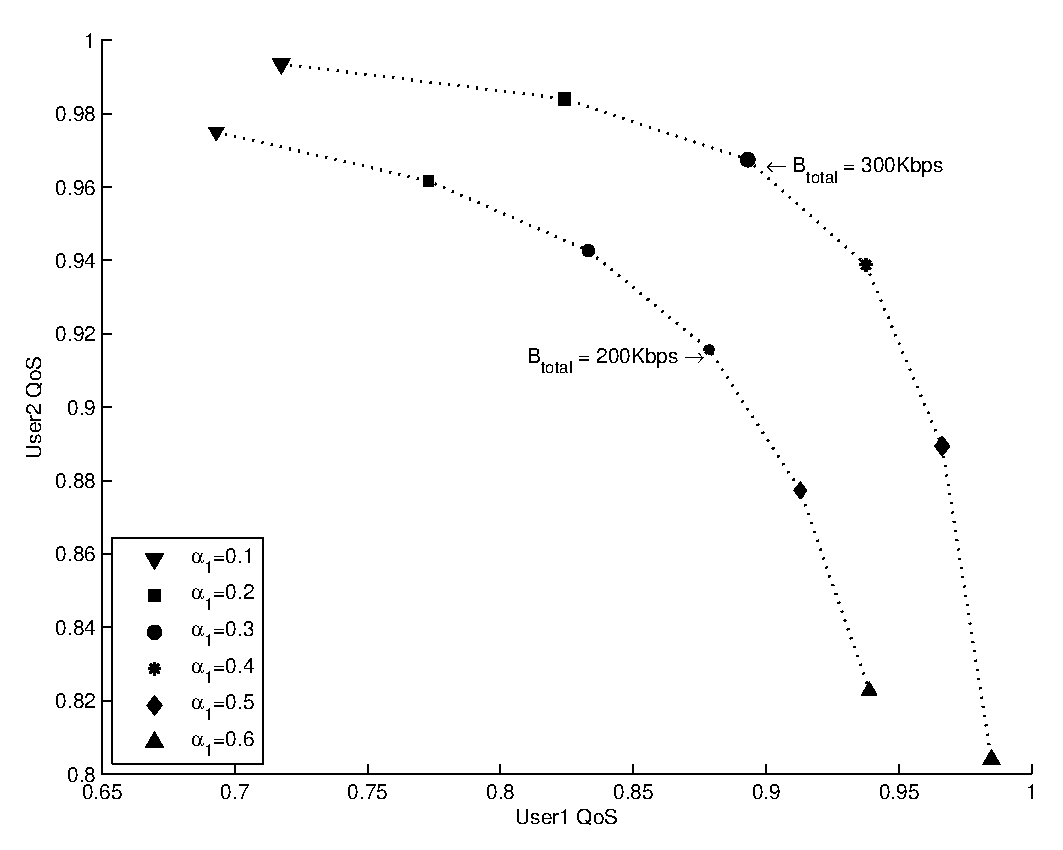
\includegraphics[width = 9cm]{chap_nash_two_users_nbs_qos.eps} 
    \caption{两用户议价能力示意图}
    \label{fig:chap_nash:two_users_nbs_qos} 
\end{figure}
那么,如何确定一个用户的议价能力是议价博弈中的一个核心问题。
在我们提出的QoS水平度量的\eqref{eqn:chap_nash:qos_definition}中,~$\rho$~被认为是一个描述用户应用特征的一个参数。
从第~\ref{chap_cacop}~章的内容中可以得知,如果~$\rho$~的值越小,那么它对资源的需求越迫切、越敏感。相反,~$\rho$~越大,对资源需求越宽松、越迟钝。
因此,我们可相应地认为,特征值~$\rho$~是用户对资源竞争能力或议价能力的一个体现。
对于某一个用户~$i$~,他的议价能力~$\alpha_i$~可定义为如下\eqref{eqn:chap_nash:bargaining_power_definition}。
\begin{align}
    \alpha_i = \frac{\frac{1}{\rho_i}}{\sum_{k=1}^n \frac{1}{\rho_k} }
    \label{eqn:chap_nash:bargaining_power_definition}
\end{align}
其中,$\rho_i$是用户$i$的特征值。
因为对于议价能力的值来说,数值越大,议价能力越强,所以,我们此处用特征值的倒数形式来定义用户的议价能力。


\section{仿真实验与结果分析}
\esection{Simulation and Results}
\subsection{仿真设置}
\esubsection{Simulation Setup}
为了验证我们的议价模型,
我们假定在一个系统中有多个用户的业务正在竞争总量为~$B_{total}$~的带宽资源。
每一个用户的业务数据是相互独立的,且每一个用户只有一种业务。

为了能够使仿真实验的结果摆脱可能是特定数据流造成的结果,我们测试了大量不同内容的真实视频的数据流。
这样可以获得更有意义的统计结果。
 我们对多个QCIF大小的标准视频测试序列,以不同的码率进行编码。
编码器采用的H.264/AVC的参考编码程序JM16 \cite{h_264_codec}。
编码的配置是采用的是Baseline档。在这个档次中,编码器使用I帧和P帧编码视频,同时支持帧内或帧间编码。
它还采用了基于上下文的自适应变长编码技术(CAVLC)。
实际应用的范围包括可视电话、电视会议和无线通信等实时的视频通信场合\cite{BiHouJie2009}。
我们实验中的编码帧结构是IPPPPP,帧率为每秒15帧。
同时,通过JM内部的码率控制算法控制编码的平均码率。
编码的结果,如 \figref{fig:chap_nash:video_psnr1}、\figref{fig:chap_nash:video_psnr2}所示。
\begin{figure}[t] 
    \centering 
  \begin{minipage}[t]{0.5\linewidth} 
    \centering 
    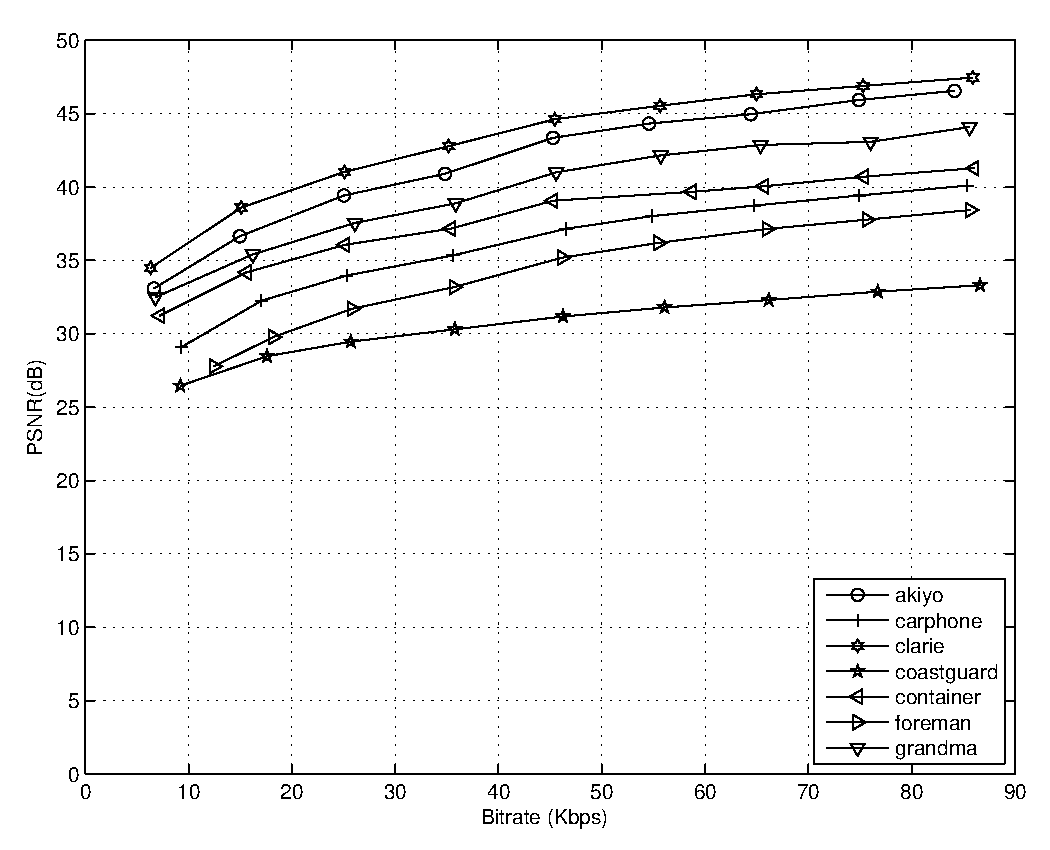
\includegraphics[width = \textwidth]{chap_nash_videobitrate_psnr1.eps} 
    \caption{视频流编码结果1} 
    \label{fig:chap_nash:video_psnr1} 
  \end{minipage}% 
  \begin{minipage}[t]{0.5\linewidth} 
    \centering 
    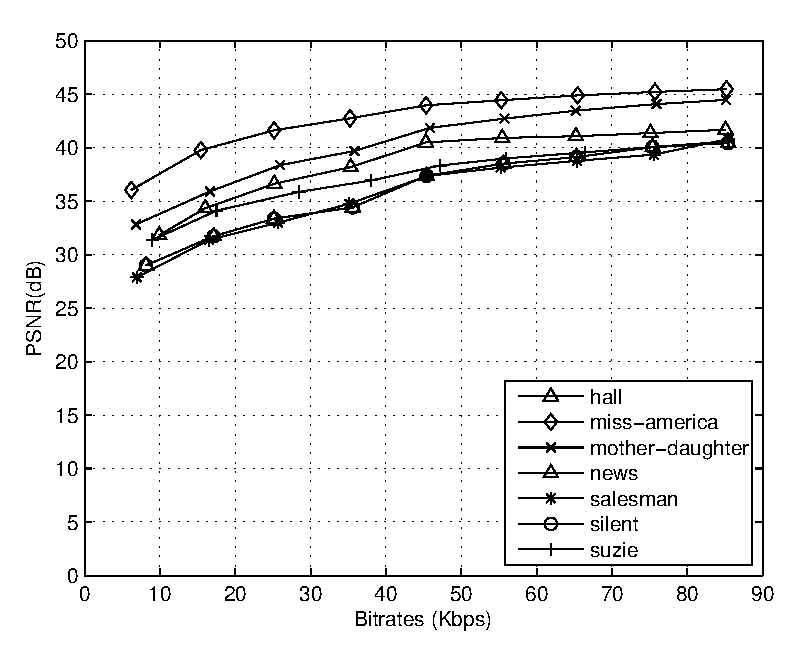
\includegraphics[width=\textwidth]{chap_nash_videobitrate_psnr2.eps} 
    \caption{视频流编码结果2} 
    \label{fig:chap_nash:video_psnr2} 
  \end{minipage} 
\end{figure}

根据编码的结果,我们先将以最大码率的PSNR为分母对每一个码率下的PSNR值做归一化处理。
然后,再通过第\ref{chap_cacop}章介绍的拟合方式,如\eqref{eqn:chap_nash:qos_level_video}所示,对业务特征值~$\rho$~进行估计。
\begin{equation}
QoS = \frac{PSNR_b}{PSNR_B} \approx \frac{1- e^{-\rho \frac{b}{B} }}{1-e^{-\rho}}, \rho > 0
\label{eqn:chap_nash:qos_level_video}
\end{equation}
这些视频业务的特征估计值,如表\ref{tab:chap_nash:before_simulation} 第二列所示。
然后,以这些估计出来的特征值,计算出相应的每一个议价能力~$\alpha_i$~,如表\ref{tab:chap_nash:before_simulation}第三列所示。
对于这些视频业务的最小资源需求~$B_i^{\min}$~,我们设定PSNR约为30的码率。
对于它们的正常资源需求为~$B_i^{req}$~,我们假设为PSNR约为40的码率。
如表\ref{tab:chap_nash:before_simulation}中最后两列所示。
从表中的议价能力值的分布变化可以看出,图像画面运动相对剧烈一些的视频,如Foreman,Mobile,
对资源需求强烈,议价能力也相应强。而那些画面相对平稳的,如Akiyo,Miss America,这些视频对资源的议价能力相对弱。
\begin{table}[tb]
    \wuhao
    \centering
    \caption{实验的各项配置参数}
    \begin{tabular*}{0.98\textwidth}{l p{0.18\textwidth}  p{0.18\textwidth}  p{0.2\textwidth}  p{0.2\textwidth} } 
    \toprule
    视频名称 &特征参数~$\rho$~ & 议价能力~$\alpha_i$~ & 最小需求~$B_i^{\min}$ ~ & 正常申请~$B_i^{req}$~ \\
    & & & (Kbps) & (Kbps) \\
    \midrule
Akiyo           	 & 11.0204 & 0.0588 & 6.65 & 14.96  \\ 
Carphone        	 & 8.8125 & 0.0735 & 9.30 & 35.61  \\ 
Clarie          	 & 13.4664 & 0.0481 & 6.35 & 15.10  \\ 
Coastguard      	 & 11.9966 & 0.0540 & 35.78 & 86.62  \\ 
Container       	 & 13.2893 & 0.0487 & 7.21 & 25.14  \\ 
Foreman         	 & 6.7800 & 0.0955 & 18.23 & 46.19  \\ 
Grandma         	 & 12.3114 & 0.0526 & 6.79 & 16.24  \\ 
Hall            	 & 10.1353 & 0.0639 & 9.93 & 25.20  \\ 
Miss America    	 & 19.4561 & 0.0333 & 6.21 & 15.45  \\ 
Mobile          	 & 4.8107 & 0.1346 & 85.08 & 127.62  \\ 
Mother\&daughter	 & 12.4678 & 0.0519 & 6.83 & 16.67  \\ 
News            	 & 8.6412 & 0.0750 & 17.16 & 45.40  \\ 
Salesman        	 & 8.2941 & 0.0781 & 16.53 & 35.16  \\ 
Silent          	 & 8.6412 & 0.0750 & 17.16 & 35.58  \\ 
Suzie           	 & 11.3603 & 0.0570 & 8.99 & 28.45  \\ 
    \bottomrule
         \end{tabular*}
    \label{tab:chap_nash:before_simulation}
\end{table}

为了比较我们所提出的议价博弈方案的性能,我们测试了其它两种典型的资源分配的方案,一种是按用户数目平均资源分配方案(Equal Allocation Solution,EAS),
另外一种是由学者Park和van der Schaar提出的另外一种纳什分配博弈模型 (Kalai–Smorodinsky  bargaining  solution),此处标记为KSBS \cite{ParkVanderSchaar2007}。此处,我们的方案记作QoS-NBS方案。
为了模拟一个在系统业务繁忙且资源缺乏的情况,我们将资源总量设置为业务最小需求之和的~$1.1$~倍的情况。
为了对这三种方案进行标准化的比较,我们对分配的带宽值用JM编码器进行重新编码,最终得到视频评价一般指标~PSNR。

\subsection{结果与分析}
\esubsection{Results and Analysis}
仿真的结果如 表\ref{tab:chap_nash:resource_allocation_comparision} 所示。
其中,应该注意到“分配码率”这一列,标有两个值。没有括号的值是我们编码前在编码配置文件中设置的码率,有括号的值是JM编码器编码过程结束后统计出的真正编码码率。
例如,对于视频Carphone,它对于EAS方案的设置码率为18.93,而最后真正编码码率为19.22。
这是因为JM编码器的码率控制单元不能够精确地把码率控制到比特级,而只能控制在一个比较小的范围内。
我们从表\ref{tab:chap_nash:resource_allocation_comparision} 中结果也可以看到,大多数视频的真正的编码码率比配置文件中设置的编码码率会稍大一些。
因此在实际的应用中,要注意到这个不同,提前设置一部分余量。
\begin{table}[tb]
    \wuhao
    \centering
    \caption{资源分配方案结果比较}
    \begin{tabular*}{\textwidth}{p{3cm}llp{2.5cm}lll}
    \toprule
    视频名称 & \multicolumn{3}{c}{设定分配码率(真实编码码率)(Kbps)} &  \multicolumn{3}{c}{PSNR(dB)} \\
    \cmidrule{2-7}
             &  EAS & KSBS & QOS-NBS&  EAS & KSBS & QOS-NBS \\
    \midrule
Akiyo                & 18.93(18.91)& 8.37(9.52)&8.17(9.36)  &37.69  &34.40  &34.35 \\ 
Carphone             & 18.93(19.22)& 11.02(13.96)&11.20(13.55)  &32.67  &31.00  &31.03 \\ 
Clarie               & 18.93(19.14)& 8.07(8.51)&7.59(8.40)  &39.77  &36.20  &36.06 \\ 
Coastguard           & 18.93(21.36)& 37.50(38.34)&37.17(38.09)  &28.87  &30.47  &30.45 \\ 
Container            & 18.93(19.12)& 8.93(10.50)&8.47(9.83)  &35.13  &32.93  &32.72 \\ 
Foreman              & 18.93(21.48)& 19.95(22.51)&20.70(22.92)  &30.70  &30.97  &31.09 \\ 
Grandma              & 18.93(19.70)& 8.51(9.89)&8.15(9.60)  &36.81  &33.91  &33.82 \\ 
Hall                 & 18.93(19.06)& 11.65(13.80)&11.58(13.80)  &34.90  &33.33  &33.33 \\ 
Miss America         & 18.93(19.40)& 7.93(8.37)&7.07(7.70)  &40.68  &37.16  &36.97 \\ 
Mobile               & 18.93(27.92)& 86.80(87.06)&88.56(89.98)  &24.37  &29.96  &30.12 \\ 
Mother\&daughter     & 18.93(19.92)& 8.55(9.85)&8.17(9.69)  &37.35  &34.13  &34.06 \\ 
News                 & 18.93(19.21)& 18.88(19.20)&19.10(20.35)  &32.51  &32.51  &32.94 \\ 
Salesman             & 18.93(19.63)& 18.25(19.21)&18.55(19.34)  &32.10  &32.01  &32.04 \\ 
Silent               & 18.93(20.76)& 18.88(20.76)&19.10(20.76)  &32.61  &32.61  &32.56 \\ 
Suzie                & 18.93(21.80)& 10.71(14.01)&10.46(13.89)  &34.89  &33.13  &33.08 \\ 
\bottomrule
    \end{tabular*}
    \label{tab:chap_nash:resource_allocation_comparision}
\end{table}
从表\ref{tab:chap_nash:resource_allocation_comparision} 中结果中还可看出,由于使用了更加合理的分配方案,方案KSBS和QoS-NBS方案对于那些运动剧烈的视频流的资源要求会给予更合理的对待。
例如,对于视频Mobile,KSBS和QoS-NBS分别使用了87.06Kbps和89.98Kbps的资源来应对,从而使得它们的PSNR值比EAS方案高出5.59dB和5.75dB,
很大程度上改善了视频质量。

为了更进一步对三者进行比较。我们对这些结果做了统计处理,如表\ref{tab:chap_nash:statis_three_schemes} 所示。
如果表面上单从平均PSNR来看,EAS方案好象最优,它超过了其它两个方案。
但是,这种性能优势的取得是通过将过多带宽资源分配给那些本来QoS质量已经较好的视频业务,使这些视频的质量达到锦上添花的效果。
例如,象Miss America的PSNR达到了40dB。
然而,对那些确实需要更多带宽资源的业务却没有给予足够的资源支持,导致其质量较差,如Mobile的PSNR低到了24dB。
EAS方案的这种表面上的用户公平性,其实并不是真正合理的公平,也不能使用户真正满意。
如果从我们定义的归一化QoS指标中,更容易看到这一点,如表\ref{tab:chap_nash:qos_3_schemes}所示。 
对于视频Mobile,它的QoS明显跌到了0.9以下。
\begin{table}[htbp]
    \wuhao
    \centering
    \caption{三种方案的统计结果比较}
    \begin{tabular*}{\textwidth}{ p{.2\textwidth}p{.25\textwidth}p{.25\textwidth}p{.3\textwidth}}
        \toprule
        & PSNR均值(dB) &PSNR方差(dB) &总带宽需求(Kbps) \\
        \midrule
        EAS & 34.07 & 18.06 & 511.05 \\
        KSBS &32.98 & 4.06 & 494.73 \\
        QoS-NBS & 32.97 & 3.74 & 494.62 \\
        \bottomrule
    \end{tabular*}
    \label{tab:chap_nash:statis_three_schemes}
\end{table}

从表\ref{tab:chap_nash:statis_three_schemes}中第二列的方差也可以清晰地看到这一点。
EAS的方差高达18dB。这说明用户的视频质量分布较大。
相比较而言KSBS方案与QoS-NBS方案较好,方差较小。用户的视频质量比较集中,且相差不大。其中,我们的方案QoS-NBS,方差可以降到4dB以下,同时PSNR的均值又可与KSBS的结果相当。
这说明,QoS-NBS方案对于单个用户的资源需求给予了更公平的对待。
即,对那些真正需要较多带宽资源的用户充分给予资源,保证他们所接受到的服务质量;
对于那些对资源需求较少的用户也给予了足够的带宽,让他们也接受到满意的服务质量。
与此同时,QoS-NBS的方案在系统资源的总量上没有增加,保持在494.62Kbps的位置,且比KSBS方案的总量略少一些。
这些结果说明,我们的模型及议价能力的定义方法不但可以兼顾业务特征差异较大的用户,也能较好地对系统所能提供的资源进行充分的利用。
总的来说,我们所提出的纳什议价博弈模型对资源竞争的描述与用户议价能力的考量是合理的。在实验中,我们通过纳什议价博弈所得到的资源分配方案在综合性能上优于其它两者的方案。

\begin{table}[htbp]
    \wuhao
    \centering
    \caption{归一化QoS水平比较}
    \begin{tabular*}{\textwidth}{ p{.2\textwidth} p{.25\textwidth} p{.25\textwidth} p{.25\textwidth} }
        \toprule
     视频名称&   EAS& KSBS & QoS-NBS \\
     \midrule
Akiyo           	 & 1.00 & 1.00  &1.00\\ 
Carphone        	 & 1.00 & 1.00  &1.00\\ 
Clarie          	 & 1.00 & 1.00  &1.00\\ 
Coastguard      	 & 0.97 & 0.98  &0.98\\ 
Container       	 & 1.00 & 1.00  &1.00\\ 
Foreman         	 & 1.00 & 1.00  &1.00\\ 
Grandma         	 & 1.00 & 1.00  &1.00\\ 
Hall            	 & 1.00 & 1.00  &1.00\\ 
Miss America    	 & 1.00 & 1.00  &1.00\\ 
Mobile          	 & 0.89 & 0.93  &0.93\\ 
Mother\&daughter	 & 1.00 & 1.00  &1.00\\ 
News            	 & 1.00 & 1.00  &1.00\\ 
Salesman        	 & 1.00 & 1.00  &1.00\\ 
Silent          	 & 1.00 & 1.00  &1.00\\ 
Suzie           	 & 1.00 & 1.00  &1.00\\ 
\bottomrule
    \end{tabular*}
    \label{tab:chap_nash:qos_3_schemes}
\end{table}



\iffalse
\fi

\section{本章小结}
\esection{Chapter Summary}
本章我们提出了一个基于纳什议价博弈的资源竞争模型及资源分配算法。
首先,我们介绍了议价博弈中的基本概念。
然后我们提出了一个新的资源分配议价博弈模型,其中包括用户的效用定义,用户的分歧点设置等。
通过对模型的定义及相关的理论分析,证明我们所提出的模型满足纳什议价公理所提出的约束。
然后,讨论了用户议价能力对博弈结果的影响,提出了以用户应用特征参数值为基础的议价能力的具体定义。
最后结合仿真实验,对所提出的算法进行了验证。
结果表明,所提出的模型与分配算法,可以有效地描述多用户在资源竞争中相互依存的关系,而且得到的纳什议价解可更合理、更公平地解决用户资源分配的问题。



%
\graphicspath{ {../body/bayesian_figures/}}
\chapter{基于连续业务类型的Bayesian博弈资源分配算法}
\echapter{Resource Allocation Algorithm with Bayesian Game}
%\label{chap_bayesian_game}
\par 
本章的目的是,在用户信息不完备的情况下,通过用户博弈的方式
研究用户类型对无线资源分配与管理的影响。
我们首先提出一个新的业务类型描述方式。
与以往的离散业务类型描述方法不同,我们将用户的业务类型描述成一个连续的随机变量。
然后建立了一个基于Bayesian博弈的竞争与决策分析模型。
这个模型可以有效地描述在不完备信息下的用户资源竞争的情况。
通过理论分析来研究用户的业务类型对博弈结果的影响。
通过理论分析得知,建立适当的收益与惩罚机制,可以激励用户根据自身的业务情况做出理性的分析和决策;
既可以保证自身的服务质量,又能让资源得到充分利用。
%
\section{引言}
\esection{Chapter Preface}
由于无线资源稀缺,研究者在无线资源分配及管理方面做了许多意义的工作。
近年来,博弈论做为经济学家常用的数学方法也被引入到无线网络技术研究领域,
特别是针对Ad Hoc网络或无线传感器网络\cite{Srivastava:2005}\cite{FangBensaou2004}。
博弈论的本质是通过数学模型来研究多个利益冲突的理性个体如何调整自己行为的理论。
通过构造合适博弈论模型及其博弈规则,可以引导自私但又理性的个体做出既有利于自已又利于其他参与者的决策。
例如,在多媒体码率分配问题中,用户往往为了保证自身最佳的服务质量,会过多地占用系统的资源,
进而导致整个系统性能的下降。
为此,学者Zhang和Liu针对这个问题,提出竞价博弈及相应的税制机制来限制用户这种过分贪婪的行为\cite{ZhangLiu2011}。

但是,这些方法都通常会有一个比较严格的假设:
在这类博弈中,每个博弈参与者或用户都要具有其他参与者或用户的完备信息。
并且,在博弈过程中,设置一个集中控制的单元负责传递用户之间的各种信息。
例如,在文献\cite{ZhangLiu2011}中,用户的各种私有信息,收益函数的参数等等都要在用户之间进行交换。
这样会导致大量的信息在用户之间传送。
这类博弈分析模型称之为完备信息下博弈模型。
通常,在博弈论研究中,所有参与者知识完备的假设是一个简单而又恰当的近似。
在有些实际的问题中,这种假设过于理想和完美。
另一方面,
因为随着移动互联网的发展,用户业务种类越来越多,越来越细致。
所以,想在资源分配之前,通过集中控制单元准确获取所有用户对资源的精确需求比较困难。
博弈论中有这样一种类型的博弈:一些参与者可能不知道其他参与者的收益。
这种类型的博弈被称之为“不完全信息的博弈”,或者被称为“Bayesian博弈”。

在本章中我们利用这种新的分析模型:Bayesian博弈分析模型,对系统中参与者的行为进行引导。
这种分析模型与完备信息博弈模型不同。
每个用户除了对自身的情况一清二楚之外,对参加博弈的其他用户的信息并不十分了解。
也就是说他所得到的其他用户信息是不完整的;或是说,每个用户的私有信息是受到一定程度的保护。

\section{业务类型与博弈模型}
\esection{Traffic Type and Game Model}
\subsection{离散与连续的业务类型}
\esubsection{Discrete and Continous Traffic Type}
目前,绝大多数的文献对于用户业务的类型讨论都是基于离散的分类形式。
例如,在早期的无线GSM网络中,话音几乎是唯一的业务。
随着网络技术的发展,除了话音外,文字、图片和视频等数据业务相继出现。
不同阶段的通信标准也根据其特点,规定了业务的种类。
比如,3GPP定义了四种基本业务类型,即会话类业务、流媒体业务、交互类业务和背景类业务。
IEEE802.16e中定义了这五种业务类型:UGS,rtPS,ertPS,nrtPS,BE。
在分类的原则上,有的的分类是指从应用层的角度来看待网络承载的数据,例如视频或声音。
有的分类是从网络传输的角度来看。不同的业务类型代表了不同业务对网络性能的要求,如对带宽、时延等等。
假设业务分类可以从概论论的角度来看,那么用户所承载的业务类型的一切可能的结果(离散的)也就可以组成的集合是一个样本空间~$\Omega$~,
那么空间中元素就可以对应为目前网络传输中的一种业务类型定义。

然而,我们如果仔细思考就会发现,这种离散的业务分类方法是有很大的局限性:过于笼统。
譬如,对于同一个视频片段,不同的编码器(MPEG4,H.264,H.265)或同一种编码器的不同编码设置参数都会对视频流的结果产生影响。
对于物理层调制编码,不同的信道模型和编码方法也同样会对传送的数据产生影响。

所以,我们认为除了原有的离散式的业务类型定义以外,还可以将这种离散式分类方法推广到连续式的业务分类方法。
这可能更接近业务本来的面目。
在连续的情况下,业务类型其实是一个概率意义上的随机变量~$X$~,并且服从某个概率分布~$F(x)$~。
每一种现实存在的业务类型都可以对应这个随机的变量的一个取值。
下面我们将这种业务分类连续定义思想应用到Bayesian博弈的分析模型中,并考察业务类型对博弈结果的影响。

\subsection{博弈模型}
\esubsection{Game Model}
假设在一个无线网络基站的覆盖范围内,目前有~$N$~个在线用户正在共享无线资源进行通信。
为了能够更加公平且有效的使用资源,基站控制器会在有新的用户进入的时候,
触发一次资源调整的方案。调整的目的是让用户根据目前自身的业务情况,重新申请合适的资源数量,
避免一些用户长期大量占用资源。
例如,在IEEE802.16标准中,
基站控制器可以通过引导各个用户投票来竞争所需要的资源。
但是由于资源有限,随着用户的数目逐渐增多,竞争就会加剧。
有时会出现先接受服务的用户为了保证自身的服务质量,申请多于自身需求资源且不加以释放。
如果对这种贪婪用户的情况不能有效地加以处理,那么结果会让整个系统的资源利用率恶化。
为了能从机制上规范所有用户的资源使用行为,改变其自身的资源过多占用策略。
我们希望通过Bayesian博弈的方式,引导用户根据自身真实的需求进行理性的资源申请和使用。

对于我们博弈模型,我们首先做如下的假设:
\begin{itemize}
    \item 假设博弈参与者业务类型可以与“参与者成本”相对应。也就是说,我们使用“参与者成本”这个随机变量来表征参与者的业务类型特征。
    \item 假设代表参与者成本的随机变量是独立同分布的,并且其累积概率分布函数~$P(\cdot)$~在区间~$[C_{\min}=0, C_{\max}=1]$~是连续增函数,
    \item 假设每个参与者自身的成本的具体取值是私有的知识,其他的参与者并不知道。
    这里需要注意是,参与者虽然不知道其他参与者成本随机变量的具体数值,但是知道这个随机变量的分布函数。
    之所以做这样假设的原因是,在实际中我们是通过统计的方法获得参与者类型的概率分布。这个信息是公共知识。
    \item 假设模型中的参与者的收益函数也是公共知识。这个信息被所有博弈参与者提前广播通知到的。
\end{itemize}

整个资源分配的过程分成两个步骤。
第一步,是用户选择与博弈阶段。
资源分配单元要征求所有~$N$~个博弈参与者的意见,是否参与本次的资源分配调整过程。
每个参与者都要在这个博弈过程中做出这样的决策:是否同意根据目前自身的情况,只分配最低限度的资源占用数量,从而释放出剩余的资源。
相应的,参与者有两种选择:“慷慨”(Generosity)或是“自私”(selfishness)。
如果选择“慷慨”,系统将按他的所需要的最低资源需求量进行配给。
如果选择“自私”,系统将按他目前申请的资源需求量进行配给。
第二步,资源分配的实施过程。资源分配单元按照参与者在第一步的决定分配物理意义上的无线资源,如带宽或子信道。

首先,我们定义博弈的策略。
显然,参与者在第一步中的选择是关键。
这种选择形式是典型的~$0-1$~决策。
对于任意一个参与者而言,他的策略选择可以用变量~$s_i$~来描述,如\eqref{eqn:chap_bayesian_strategy_definition}所示。
\begin{align}
    s_i = \begin{cases}
        1, \qquad\text{慷慨}\\
        0, \qquad\text{自私}\\
    \end{cases}
    \label{eqn:chap_bayesian_strategy_definition}
\end{align}
其中,此函数的定义域是成本区间~$[C_{\min}, C_{\max}]$~,值域是集合~$\{0,1\}$~中取任意一个值。
“~$1$~”表示参与者愿意“慷慨”;“~$0$~”表示参与者“自私”;
~$i$~表示参与者的序号索引。

然后,我们定义博弈中的参与者收益。
从前面的叙述中可知,在资源有限的情况下,这种博弈本质是一种零和博弈。
每一个自私的参与者希望别的参与者选择“慷慨”,
而自身选择“自私”,不改变目前资源的占用数量。
如果有参与者~$i$~选择“慷慨”,那么我们认为其他选择“自私”的参与者都会因他的“慷慨的行为”而获益~$b=1$~。
而这名博弈参与者所得的收益为~$b-c_i= 1-c_i$~。
显然在此情况下,选择“慷慨”的参与者收益要小于选择“自私”的参与者收益。
但是,为了鼓励参与者选择“慷慨”而且研究选择“慷慨”的参与者数目对博弈结果的影响,我们做如下的假定:
如果选择“慷慨”的参与者数目小于$m$; 其它的参与者都选择“自私”,
不愿意“牺牲”自己的利益,那么所有参与者的获益都将是~$b$~为~$0$~。

那么,对于参与者~$i$~来说,他的收益函数定义为\eqref{eqn:chap_bayesian_player_payoff}:
\begin{equation}
 u_i(s_i, s_{-i}, c_i, m) = s_i\cdot (1 - c_i) + (1-s_i) \cdot \Phi(s_{-i},m)
\label{eqn:chap_bayesian_player_payoff}     
\end{equation}
其中,记号~$-i$~表示除参与者~$i$~之外的其它所有参与者。
记号~$s_{-i}$~表示其他参与者~$-i$~的策略选择集合。
~$c_i$~表示参与者~$i$~的成本。
~$\Phi(s_{-i},m)$~表示对于其他的参与者,是否有~$m$~个参与者选择“慷慨”,如\eqref{eqn:chap_bayesian:m_users_agree}定义所示。
\begin{align}
    \Phi(s_{-i,},m) = \begin{cases}
        1, \qquad \text{if } \sum s_{-i} \ge m;\\
        0, \qquad \text{others};
    \end{cases}
    \label{eqn:chap_bayesian:m_users_agree}
\end{align}

%
\section{Bayesian博弈分析}
\esection{Analysis of Bayesian Game}
对于每一个理性且自私的博弈参与者,他总想通过自己的选择来使自己的收益最大化。
可以表示为~$\max(u_i)$~。
对于所有参与者的选择来说,最后的纯策略均衡可以用一个策略向量~$( s_1^*(c_1^*),\ldots, s_N^*(c_N^*) )$~来描述。
其中,策略~$s_i^*(c_i^*)$~使得~$u_i$~达到最大值。

但是,如果直接求解收益最大化,会使问题本质变成是一个$N$目标优化的极其复杂问题,这是我们所不希望看到的。
所以,为了避免陷入这样情况,我们转而求解参与者的期望收益最大化问题,~$\max\{E(u_i)\}$~。
最后求解出所谓的混合策略。混合策略是纯策略上的一种概率分布。每个博弈参与者的随机化及其他参与者的随机化是统计独立的。
相应的Bayesian博弈的解就是博弈参与者选择“慷慨”或“自私”的概率。

下面我们来具体分析这个博弈。
首先我们引入一个均衡概率的定义~$\theta_{-i}(m)$~。
它表示对于参与者~$i$~而言,至少有~$m$~个其他的参与者的决定是“慷慨”的概率。
实际上,通过这个概率定义的引入,我们使得博弈参与者~$i$~的决策与其它博弈参与者的决策行为相关联。
这样,参与者关于其它参与者的判断可以由自己的收益函数来决定。
同时,也可以看作是,通过这个定义来表征参与者之间的博弈行为。
这个概率的具体表达式如\eqref{eqn:chap_bayesian:at_least_one_probability}所示。
\begin{equation}
    \theta_{-i}(m) = \hbox{Prob} \Bigl\{ \Phi( s_{-i},m) = 1 \Bigr\}, \, m\le N-1
    \label{eqn:chap_bayesian:at_least_one_probability} 
\end{equation}
所以,对于一个给定的博弈参与者~$i$~,他的期望收益可以由\eqref{eqn:chap_bayesian_player_payoff} 
和\eqref{eqn:chap_bayesian:m_users_agree}定义为如下公式:
\begin{align}
     E(u_i) &= \theta_{-i}(m)\left[s_i(b-c_i) +(1-s_i)\right] \notag \\
     & \quad + [1-\theta_{-i}(m)] [s_i(b-c_i) + 0] \notag\\ 
     &= s_i[1-c_i-\theta_{-i}(m)] + \theta_{-i}(m)
    \label{eqn:player_expe_payoff}
\end{align}

从\eqref{eqn:player_expe_payoff}可以看出,为了使得~$E(u_i)$~尽可能大,并考虑决策的前提下,可以分成两种情况。
如果博弈参与者~$i$~的成本~$c_i$~小于~$1-\theta_{-i}(m)$~,那么参与者~$i$~的决策就是“慷慨”,也就是~$s_{i}=1$~。
如果~$c_i > 1 - \theta_{-i} (m)$~,那么参与者~$i$~会选择“自私”,~$s_i = 0$~。
那么我们也将其写为一个分段函数的形式。
\begin{align}
    s_i(c_i) = \begin{cases} 
        1, &\text{if $c_i < 1 -\theta_{-i}(m)$;}\\
        0, &\text{if $c_i > 1 -\theta_{-i}(m)$.}\\ \end{cases} 
    \label{eqn_equilibrium_strategy} 
\end{align}
从\eqref{eqn_equilibrium_strategy}可以看出,参与者~$i$~的成本对决策的影响很关键。
如果他的成本~$c_i$~在区间~$ [C_{\min}, c_i^*] $~,参与者的决策就是“慷慨”。
其中,我们把~$c_i^*$~称为均衡临界成本。
所以,参与者~$i$~选择“慷慨”概率,也就是均衡临界成本的概率~$P(c_i^*)$~,
如\eqref{eqn:chap_bayesian:equil_prob_c_i}所示。
\begin{align}
    P(c_i^*) = \hbox{Prob} \Bigl\{ C_{\min} < c_i \leq c_i^* \Bigr\} 
    \label{eqn:chap_bayesian:equil_prob_c_i}
\end{align}
而且,
%因为对于每一个博弈参与者而言,他的业务随机变量或成本随机变量而言,是独立同分布的。
因此,如果存在这样一个均衡临界成本,
%可以将~$\theta_{-i}(m)$~看作为一个二项分布的情况。
我们将\eqref{eqn:chap_bayesian:equil_prob_c_i} 代入\eqref{eqn:chap_bayesian:at_least_one_probability},
那么就有:
\begin{align} 
    \theta_{-i}(m) &= \hbox{Prob} \Bigl\{ \Phi( s_{-i},m) = 1 \Bigr\} \notag \\ 
   % &= C_{N-1}^m [P(c^*)]^m [1-P(c^*)]^{N-m-1} \notag \\
   % & \quad + \cdots + C_{N-1}^{N-1} [P(c^*)]^{N-1} [1-P(c^*)]^{N-(N-1)-1} \notag \\
   % &= \sum_{k=m}^{N-1}C_{N-1}^k [P(c^*)]^k [1-P(c^*)]^{N-k-1}
   &= P(c_1^*)P(c_2^*)\cdots P(c_{m}^*) \cdot (1-P(c_{m+1}^*)) \cdots(1-P(c_{N-1}^*)) \notag \\ 
    & \quad +  P(c_0^*)P(c_2^*)\cdots P(c_{m+1}^*) \cdot (1-P(c_{m+2}^*)) \cdots(1-P(c_{N-1}^*)) \notag \\ 
    & \quad + \cdots  + P(c_1^*)P(c_2^*)\cdots P(c_{N-2}^*) \cdot (1-P(c_{N-1}^*)) \notag \\
    & \quad +  P(c_1^*)P(c_2^*)\cdots P(c_{N-1}^*)  
    \label{eqn:chap_bayesian:two_poly_distribution}
\end{align}
\eqref{eqn:chap_bayesian:two_poly_distribution}表示了在其它参者个数为~$N-1$~的情况下,
至少存在~$m$~个参与者选择“慷慨”的概率。如果
同时,从\eqref{eqn:chap_bayesian:at_least_one_probability}和\eqref{eqn_equilibrium_strategy}可知,
均衡临界成本 ~$c_i^*$~是用户决策的关键值。它关系到用户选择的转换。
因此,均衡临界成本还要满足下面\eqref{eqn_equilibrium_cost}
\begin{align}
    c_i^* &= 1 - \theta_{-i} (m) \notag \\
     & =1 - [P(c_1^*)P(c_2^*)\cdots P(c_{m}^*) \cdot (1-P(c_{m+1}^*)) \cdots(1-P(c_{N-1}^*)) \notag \\ 
    & \quad +  P(c_0^*)P(c_2^*)\cdots P(c_{m+1}^*) \cdot (1-P(c_{m+2}^*)) \cdots(1-P(c_{N-1}^*)) \notag \\ 
    & \quad + \cdots  + P(c_1^*)P(c_2^*)\cdots P(c_{N-2}^*) \cdot (1-P(c_{N-1}^*)) \notag \\
    & \quad +  P(c_1^*)P(c_2^*)\cdots P(c_{N-1}^*) ]
    \label{eqn_equilibrium_cost} 
\end{align}
对于博弈中的任意一个~$c_i^*, i=1,\ldots, N$~,都要满足
\eqref{eqn_equilibrium_cost}。
又因为所有参与者的成本随机变量是独立同分布的,并且对于每一个~$c_i^*, i=1,\ldots, N$~
在\eqref{eqn_equilibrium_cost}等号左右两边是可以任意互相交换的。
所以对于一种分布来说,那么它们值一定相等,即~$c_1^* = c_2^* = c_3^* \cdots = c_N$~。
则我们把这个值记为~$c^*$~。
因此,我们可以将 \eqref{eqn_equilibrium_cost}改写为二项分布的形式,如
\eqref{eqn:chap_bayesian:equilibrium_cost_equation}所示。我们可以通过解这个方程来计算得出~$c^*$~。
\begin{align}  
    c^* & =  1 - [ C_{N-1}^m [P(c^*)]^m [1-P(c^*)]^{N-m-1} \notag \\
   & \quad + \cdots + C_{N-1}^{N-1} [P(c^*)]^{N-1} [1-P(c^*)]^{N-(N-1)-1} ]\notag \\
   &= 1- \sum_{k=m}^{N-1}C_{N-1}^k [P(c^*)]^k [1-P(c^*)]^{N-k-1}
\label{eqn:chap_bayesian:equilibrium_cost_equation}
\end{align}

综上所述,对于我们提出的Bayesian博弈模型而言,网络中博弈参与者成本(用户业务类型)的概率分布情况会对博弈结果起着关键的影响作用。
%%%%%%%%%%%%%%
\section{不同业务类型概率分布的分析与讨论}
\esection{Analysis and Discuss of Traffic Type Distribution}
下面,我们假设博弈参与者成本(业务类型)为两种最常见的概率分布形式,并分别对其进行分析与讨论。
\subsection{均匀分布的情况}
\esubsection{Uniform Distribution}
均匀分布是连续概率分布函数中最常见和最简单的。它在所有的概率分布中占着重要的地位。
许多实际上重要的随机变量者服从或是近似服从均匀分布。
此处,我们假设参与者的类型的概率分布~$P(\cdot)$~是在区间~$[C_{\min}=0, C_{\max}=1]$~上的均匀分布。
它的概率密度函数为
\begin{align}
    f(c) = \begin{cases} c, &\text{if ~$c \in [C_{\min}=0, C_{\max}=1]$~;}\\
        0, &\text{others}\\ 
    \end{cases} 
    \label{eqn_equilibrium_prob} 
\end{align}
其中,我们假设对于参与者的成本被认为是归一化的。
概率密度函数与分布函数图形如\figref{fig:chap_bayesian:uniform_density_scheme}和\figref{fig:chap_bayesian:uniform_cdf_schem}所示。
%%%%%%%%%%%%%%%%%%%%%%%%%%%%%%%%%%%%%%%%%%%%%%%%%%%%%%%%%%%%%%%%%%%%%
\begin{figure}[tb] 
  \begin{minipage}[t]{0.5\linewidth} 
    \centering 
    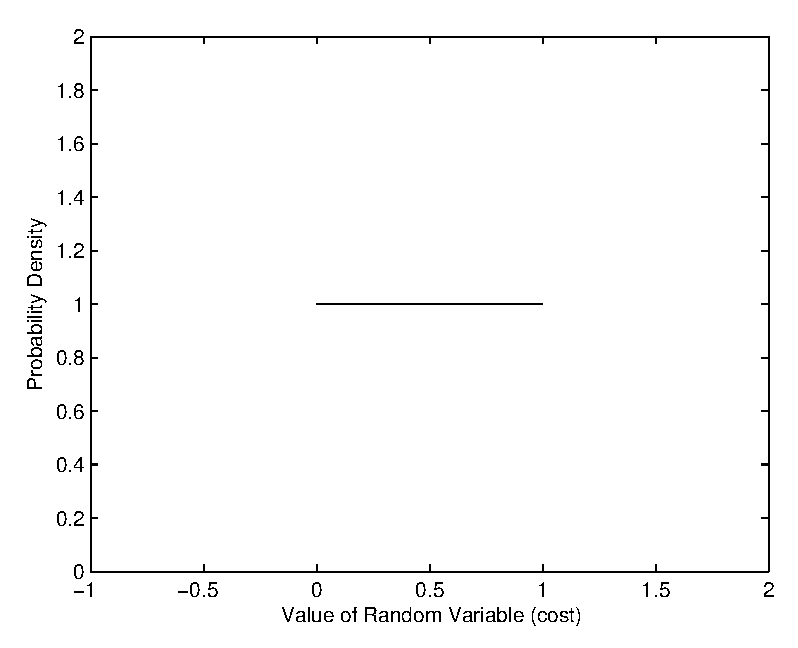
\includegraphics[width = \textwidth]{bayesian_uniform_density_scheme.eps} 
    \caption{均匀分布的概率密度函数} 
    \label{fig:chap_bayesian:uniform_density_scheme} 
  \end{minipage}% 
  \begin{minipage}[t]{0.5\linewidth} 
    \centering 
    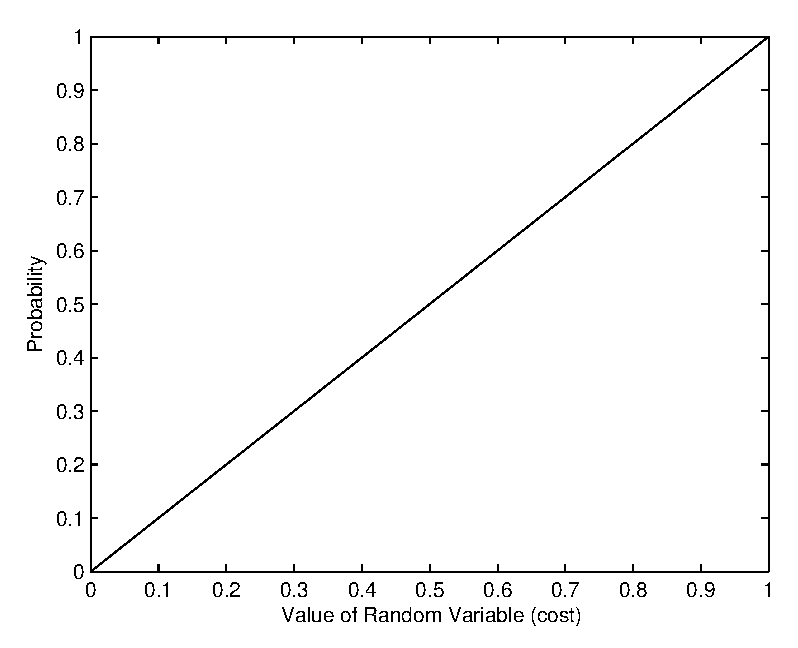
\includegraphics[width=\textwidth]{bayesian_uniform_cdf_scheme.eps} 
    \caption{均匀分布的累积概率函数} 
    \label{fig:chap_bayesian:uniform_cdf_schem} 
  \end{minipage} 
\end{figure}
则达到临界成本~$c^*$~来说,选择“慷慨”的概率为
\begin{align} 
    P(c^*) &= \text{Prob} \Bigl\{ 0 < c_i < c^*\Bigr\} \notag\\ 
    &= \frac{c^*}{C_{\max}-C_{\min}} \notag\\
    &= c^* 
    \label{eqn_probability_of_contribution} 
\end{align}
把\eqref{eqn_probability_of_contribution}代入\eqref{eqn:chap_bayesian:equilibrium_cost_equation}则有
\begin{align*} 
    c^* = 1- \sum_{k=m}^{N-1}C_{N-1}^k (c^*)^k [1-(c^*)]^{N-k-1}
\end{align*}

我们通过做图的方式来直观地讨论在均匀分布的情况下,各个参数对于临界成本和参与者决策的影响,
如\figref{fig:bayesian_user_numb_vs_contr_prob}所示。
%如\figref{fig:bayesian_user_numb_vs_contr_prob}和\figref{fig:bayesian_puni_para_vs_cont_prob}所示。
图中所涉及的奖励~$b$~,成本~$c$~都是归一化后的,且为了简单起见,~$b = 1$~。
%%%%%%%%%%%%%%%%%%%%%%%%%%%%%%%%%%%%%%%%%%%%%%%%%%%%%%%%%%%%%%%%%%%%%
\begin{figure}[tb]
\begin{centering}
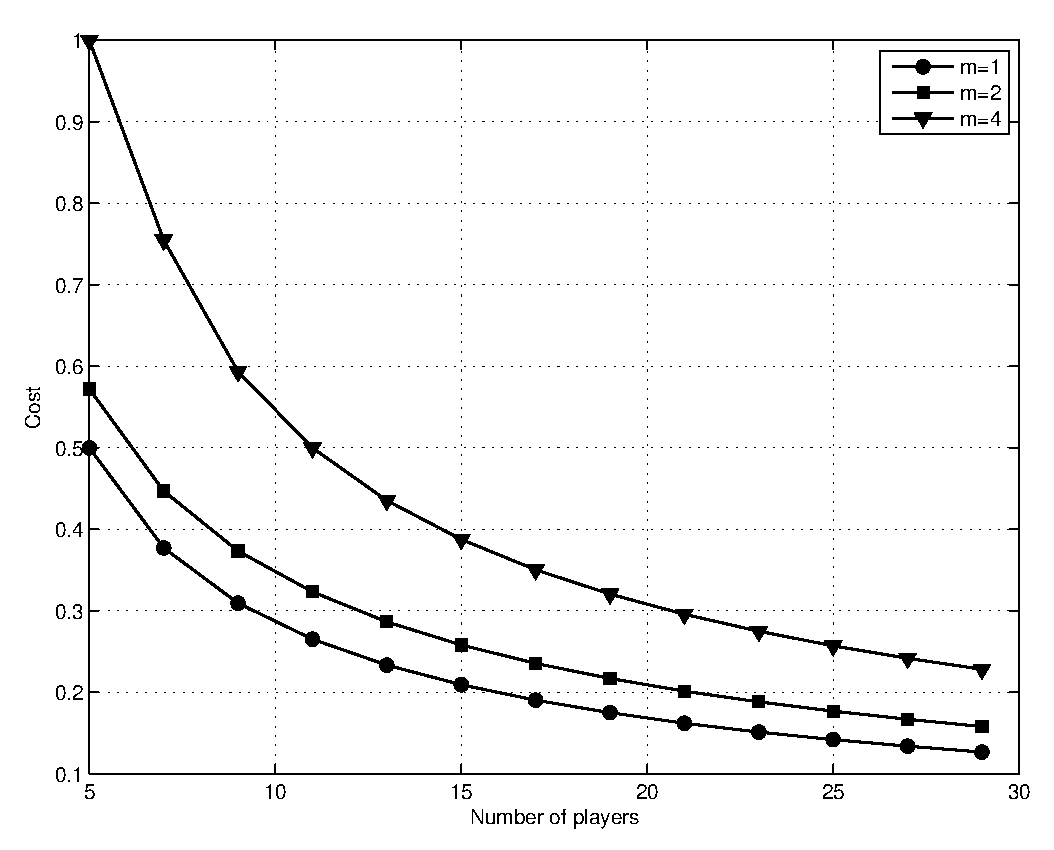
\includegraphics[scale=0.6]{bayesian_uniform_user_number_vs_contribute_probability.eps}
\caption{参与者数目与临界成本的关系(均匀分布)}
\label{fig:bayesian_user_numb_vs_contr_prob}
\end{centering}
\end{figure}
%%%%%%%%%%%%%%%%%%%%%%%%%%%%%%%%%%%%%%%%%%%%%%%%%%%%%%%%%%%%%%%%%%%%
%%%%%%%%%%%%%%%%%%%%%%%%%%%%%%%%%%%%%%%%%%%%%%%%%%%%%%%%%%%%%%%%%%%%%
%\begin{figure}[tb]
%\begin{centering}
%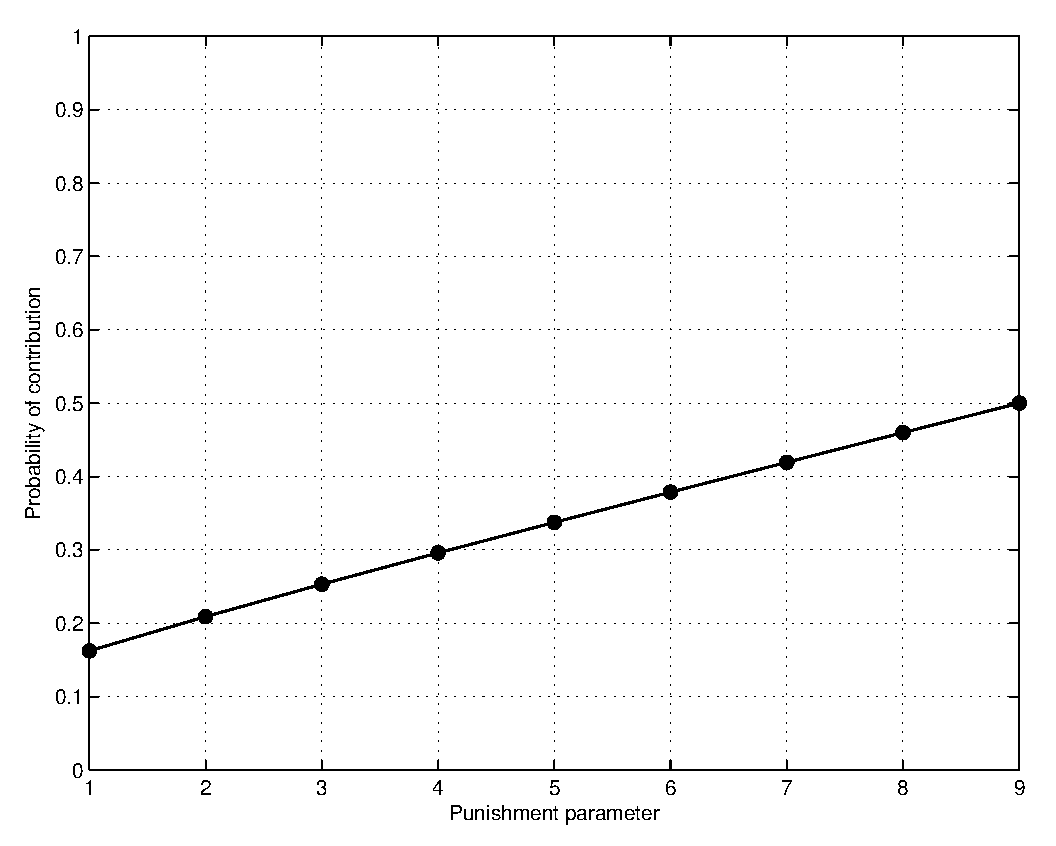
\includegraphics[scale=0.7]{bayesian_uniform_punish_parameter_vs_contribute_probability.eps}
%\caption{“慷慨”参与者数目最低要求$m$与临界成本的关系(均匀分布),$N=10$}
%\label{fig:bayesian_puni_para_vs_cont_prob}
%\end{centering}
%\end{figure}
%%%%%%%%%%%%%%%%%%%%%%%%%%%%%%%%%%%%%%%%%%%%%%%%%%%%%%%%%%%%%%%%%%%%
从\figref{fig:bayesian_user_numb_vs_contr_prob}可以看到,
当博弈的参与者总数增多时,临界成本~$c^*$~会减小。
前面我们提到,当博弈参与者的成本~$c_i$~在区间~$ [C_{\min}, c_i^*] $~,参与者的决策就是“慷慨”。
因而,最终博弈均衡中选择“慷慨”的概率~$P(c_i^*)$~也会随之降低。
这意味着,当系统中参与者较少时,参与者容易做出接受资源调整的决策。
而当系统参与者较多时,即使参与者的收益比成本高,参与者也可能会做也自私的决定。
这说明,当用户总数目多的情况下,自私的用户都希望他人来做出资源占用的调整,而自身却“自私”调整。
另外,
%从\figref{fig:bayesian_puni_para_vs_cont_prob}
可以看到,当对决策“慷慨”的数目~$m$~有最低要求时,博弈参与者的“自私”决策概率会降低。
因为大家都会担心没有人选择“慷慨”来让自己最终的收益为零。
因此在系统中设置一个能够自适应网络状态的最低“慷慨”的参与者数目,也是调节参与者选择态度的有效手段。

\subsection{正态分布的情况}
\esubsection{Normal Distribution}
对于参与者的成本类型,第二种我们假设的概率分布是正态分布。
也是一个在数学、物理及工程等领域都非常重要的概率分布。
对于参与者成本随机变量~$c$~服从一个位置参数为~$\mu$~,尺度参数为~$\sigma$~的概率分布,
通常可以记为:
\begin{align*}
    c \sim N(\mu, \sigma^2)
    %\label{eqn:normal_distribution}
\end{align*}
服从正态分布的随机变量的概率密度函数~$f(x)$~由\eqref{eqn:chap_bayesian:normoal_density}和\eqref{eqn:chap_bayesian:normoal_cdf}给出,
且其概率密度函数和概率分布函数如\figref{fig:chap_bayesian:normal_density_scheme}和\figref{fig:chap_bayesian:normal_cdf_schem}所示。
其中,与均匀分布类似的,为了将成本随机变量控制在区间~$[0,1]$~,我们假设成本概率分布的均值为~$\mu = 0.5$~,方差~$\delta = 0.1$~。
\begin{align}
    f(x) = \frac{1}{\sigma \sqrt{2\pi} } e^{ \frac{-(c-\mu)^2}{2\sigma^2}}
    \label{eqn:chap_bayesian:normoal_density}
\end{align}
\begin{align}
    F(x) = \frac{1}{\sigma \sqrt{2\pi} } \int^x_{-\infty}e^{ \frac{-(c-\mu)^2}{2\sigma^2}}
    \label{eqn:chap_bayesian:normoal_cdf}
\end{align}
%%%%%%%%%%%%%%%%%%%%%%%%%%%%%%%%%%%%%%%%%%%%%%%%%%%%%%%%%%%%%%%%%%%%%
\begin{figure}[tb] 
  \begin{minipage}[t]{0.5\linewidth} 
    \centering 
    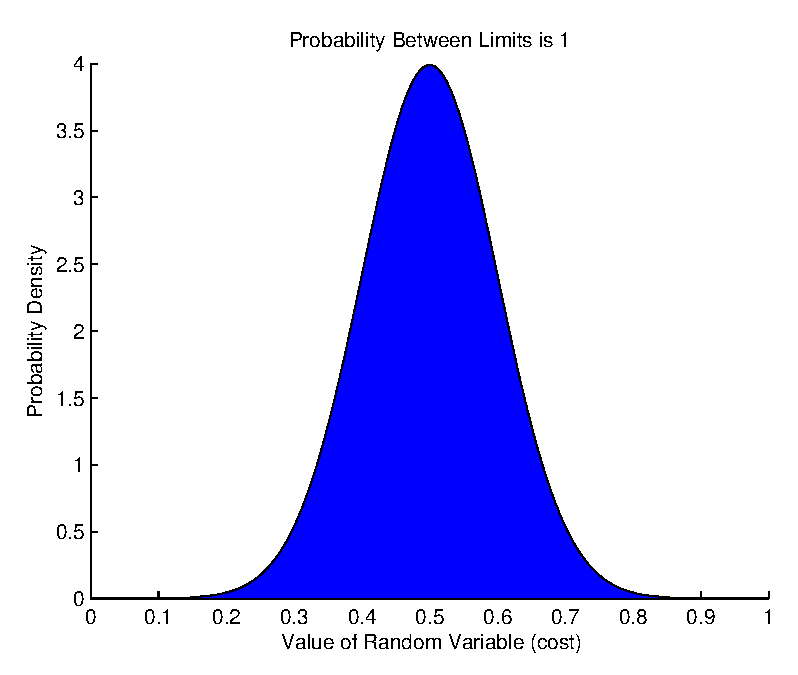
\includegraphics[width = \textwidth]{bayesian_normal_density_scheme.eps} 
    \caption{正态分布的概率密度函数} 
    \label{fig:chap_bayesian:normal_density_scheme} 
  \end{minipage}% 
  \begin{minipage}[t]{0.5\linewidth} 
    \centering 
    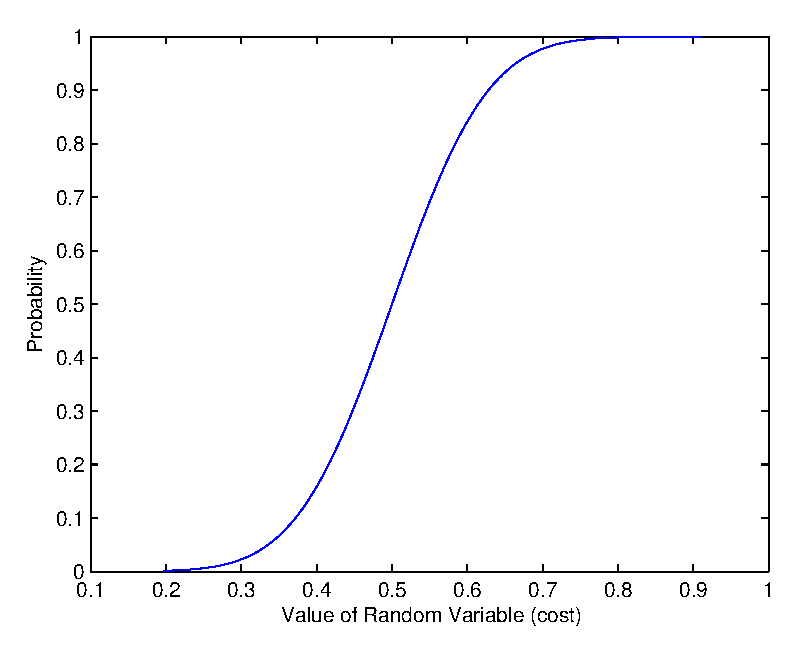
\includegraphics[width=\textwidth]{bayesian_normal_cdf_scheme.eps} 
    \caption{正态分布的累积概率函数} 
    \label{fig:chap_bayesian:normal_cdf_schem} 
  \end{minipage} 
\end{figure}
类似的,如果将\eqref{eqn:chap_bayesian:normoal_cdf}代入\eqref{eqn:chap_bayesian:equilibrium_cost_equation},
则有,
\begin{align} 
    c^* &= 1- \sum_{k=m}^{N-1}C_{N-1}^k \left\{\left[ \frac{1}{\sigma \sqrt{2\pi} } \int^x_{-\infty}e^{ \frac{-(c^*-\mu)^2}{2\sigma^2}})\right]^k \right. \notag \\
    & \qquad \left. \quad \cdot \left[1- \frac{1}{\sigma \sqrt{2\pi} } \int^x_{-\infty}e^{ \frac{-(c^*-\mu)^2}{2\sigma^2}}\right]^{N-k-1} \right\}
     \label{eqn:chap_bayesian:cost_normal_distribution_equation}
\end{align}
由于正态分布函数概率密度函数不能显式积分,所以我们只能通过数值求解的方式,将收益参数、“慷慨”人数最低值、参与者数目与均衡成本关系画出来。
如\figref{fig:bayesian_normal_user_numb_vs_contr_prob}和\figref{fig:bayesian_normal_puni_para_vs_cont_prob}所示。
%%%%%%%%%%%%%%%%%%%%%%%%%%%%%%%%%%%%%%%%%%%%%%%%%%%%%%%%%%%%%%%%%%%%%
\begin{figure}[tb]
\begin{centering}
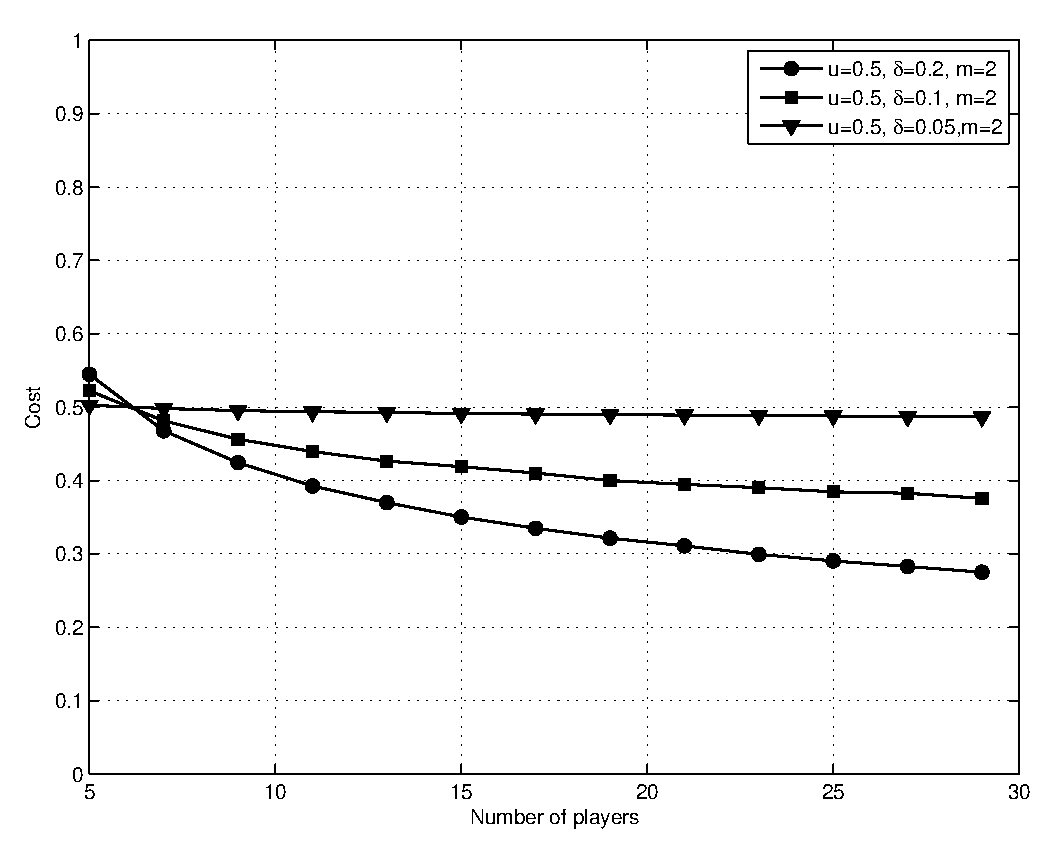
\includegraphics[scale=0.6]{bayesian_normal_user_number_vs_contribute_probability.eps}
\caption{参与者数目与临界成本的关系(正态分布)}
\label{fig:bayesian_normal_user_numb_vs_contr_prob}
\end{centering}
\end{figure}
%%%%%%%%%%%%%%%%%%%%%%%%%%%%%%%%%%%%%%%%%%%%%%%%%%%%%%%%%%%%%%%%%%%%
%%%%%%%%%%%%%%%%%%%%%%%%%%%%%%%%%%%%%%%%%%%%%%%%%%%%%%%%%%%%%%%%%%%%%
\begin{figure}[!tb]
\begin{centering}
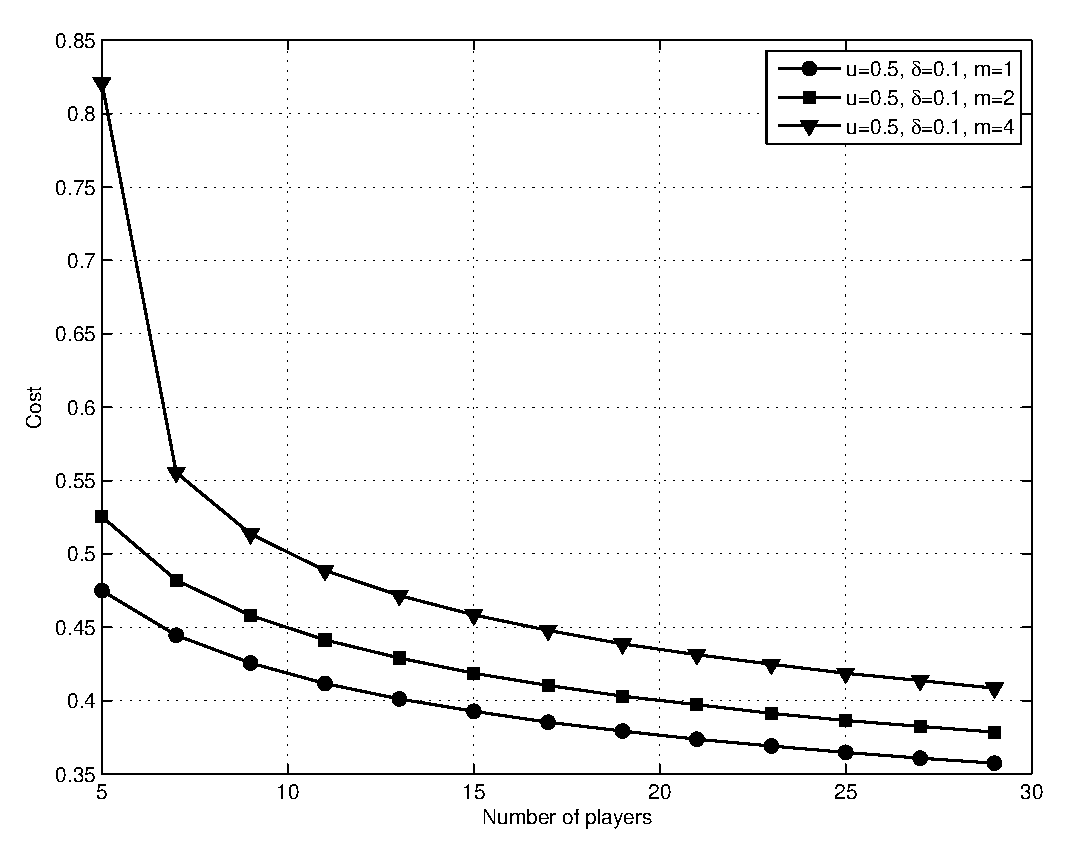
\includegraphics[scale=0.6]{bayesian_normal_punish_parameter_vs_contribute_probability.eps}
\caption{“慷慨”参与者数目最低要求$m$与临界成本的关系}
\label{fig:bayesian_normal_puni_para_vs_cont_prob}
\end{centering}
\end{figure}

与均匀分布的情况十分相似,
当博弈的参与者总数增多时,临界成本~$c^*$~会减小, 如\figref{fig:bayesian_normal_user_numb_vs_contr_prob}如示。
同样,博弈参与者选择“慷慨”的概率~$P(c_i^*)$~也会随之降低。
同理,当系统中参与者较少时,参与者容易做出接受资源调整的决策。
我们还绘制了正态分布的尺度参数~$\delta$~对临界成本的影响。
当尺度参数的取值较小时,意味着博弈参与者的类型分布集中比较集中。
从图中可以看出,用户类型集中的情况下,博弈参与者选择“慷慨”的概率也较高。
\figref{fig:bayesian_normal_puni_para_vs_cont_prob}也表明,
当对“慷慨”参与者的数目的最低值增大时,参与者决策均衡中“慷慨”的机率会增大。这一点与均匀分布一样。

\section{基于博弈的自适应业务分布资源分配算法}
\esection{Proposed Resource Allocation Algorithm with Bayesian Game}
至此,我们解决了在资源不足以致于不可能给每一个博弈参与者提供最好服务质量下,
让博弈者自己来决定可以降低自己的资源需求。

根据前面的分析,本节我们提出一个资源分配算法来满足每一个用户的需求。
资源分配单元,当有用户要申请更多的资源时,收集各个参与者的业务类型或成本信息。
根据预设的分布模型,将成本信息汇总以后,进行参数估计,求得均值与方差。
然后确定这一时间段内的分布函数的具体形式,并广播给当前服务区的用户。
用户收到本时段的分布函数后,可计算出当前的均衡成本值。
然后用这个值作为选择“慷慨”的概率,做出自身的决策。
最后将决策报告给资源分配单元,完成实际的分配工作。

此分配算法的具体流程如 算法 \ref{alg:chap_bayesian:agr_cac} 所示。
\begin{algorithm}[!htbp]
\SetAlgoLined
% assume $B_{ava}=0$\;
等待用户申请资源 \;
如果某一个用户~$i$~根据自己的当前成本~$c_i$~提出新的资源申请要求~$b_i$~ \;
\eIf {当前空闲资源可满足用户~$i$~的需求}{
通知“资源控制分配单元”,给用户申请所需的资源 \; 
}{
向当前服务的所有用户广播“成本收集”消息 \;
所有用户向 “资源控制与分配单元” 报告自己当前的成本 \;
“资源控制与分配单元”选择预设的成本随机分布模型 \;
对模型中参数进行参数估计(均值或方差) \;
将业务模型及刚才得到的参数估计广播给所有用户 \;
每个用户得到业务模型后,计算均衡成本~$c^*$~及选择“慷慨”的概率 \;
按照“慷慨”的概率值做出自己的最后决策(为了保证在线用户通信不被中断,假设如果系统中已经做过“慷慨”选择的用户不再参与本次博弈)\;
\eIf{决策为“慷慨”}{
    向资源控制与分配单元报告自己的决策和自己对资源最低要求\;
    }
    {
    向资源控制与分配单元报告自己的决策和自己目前的资源需求\;
    }
资源控制与分配单元接收到所有的回复报告\;
统计用户总的需求与目前总的资源\;
\eIf{用户总需求~$\le$~总资源供给}{
    本次资源调整成功\;
    \For{~$k=1$~ \KwTo ~$N$~}{
    给每一个在线用户分配资源\;
    }
    }{
    此次资源调整失败\;
    并通知用户~$i$~\;
    }
    本次资源调整结束\;
}
    转到 \bf 1\;
\caption{基于博弈的自适应业务分布资源分配算法} 
\label{alg:chap_bayesian:agr_cac}
\end{algorithm}

\section{仿真实验与结果}
\esection{Simulation and Results}
为了验证我们进行的理论分析结果,以及提出的分配算法有效。
我们参照基站分配资源的基本功能设计以下仿真模型。
在这个仿真模型中,包括一个资源控制与分配单元和~$N$~个用户。
这~$N$~个用户符合某个预设的业务类型分布模型,每个用户的慷慨成本为~$c_i$~。
每个用户的对资源的需求假设带宽~$b_i$~,在64Kbps到4Mbps之间取值;
并且,因为~$c_i$~是对用户而言要付出的成本,所以为了简单起见,假设每个用户对资源的最低需求为~$(1-c_i)b_i$~。

\subsection{仿真实验一}
\esubsection{Simulation Experiment I}
为了验证理论分析,我们编写了第一个仿真的脚本。
同样,我们比较两种业务分布函数,均匀分布和正态分布。
其中,正态分布的参数设置为~$\mu = 0.5, \delta^2 = 0.1$~;
最少参与者决策“慷慨”的数目设置为~$m=4$~。
为了能够得到一个统计意义的结果,仿真脚本每组运行了~$300$~次。
最后的仿真结果如
\figref{fig:chap_bayesian:normal_bandwidth_vs_user_number}至
\figref{fig:chap_bayesian:normal_bandwidth_vs_success_probability}
所示。
%%%%%%%%%%%%%%%%%%%%%%%%%%%%%%%%%%%%%%%%%%%%%%%%%%%%%%%%%%%%%%%%%%%%%
\begin{figure}[!tb] 
    \centering
   \begin{minipage}[t]{0.5\linewidth} 
    \centering 
    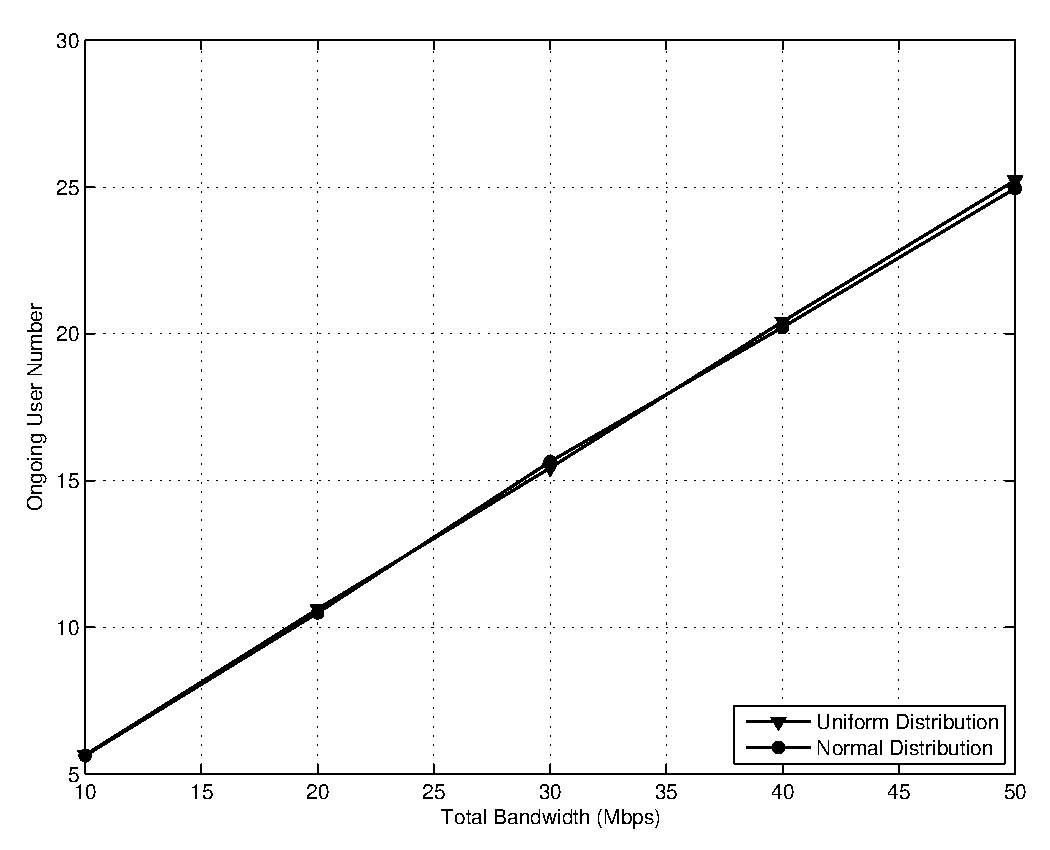
\includegraphics[width = \textwidth]{bayesian_normal_bandwidth_vs_user_number} 
    \caption{在线用户数目} 
    \label{fig:chap_bayesian:normal_bandwidth_vs_user_number} 
  \end{minipage}% 

  \begin{minipage}[t]{0.5\linewidth} 
    \centering 
    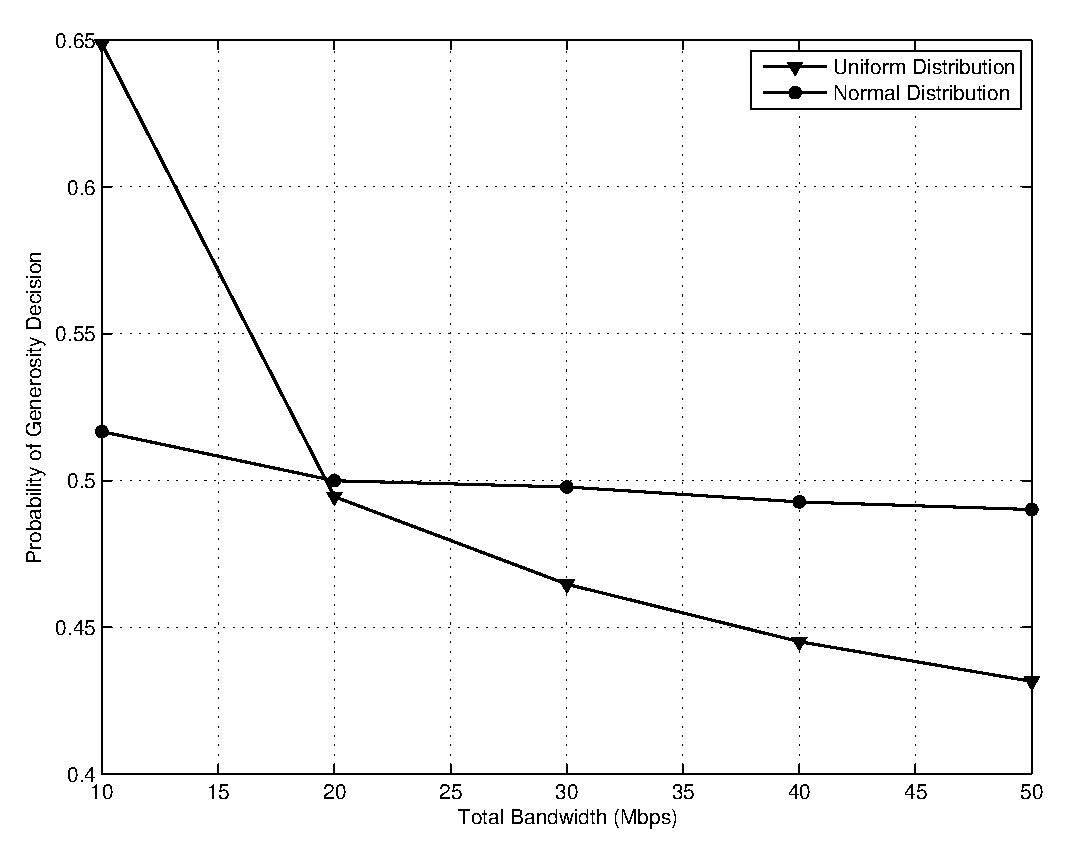
\includegraphics[width = \textwidth]{bayesian_normal_bandwidth_vs_generosity} 
    \caption{用户决策“慷慨”概率} 
    \label{fig:chap_bayesian:normal_bandwidth_vs_generosity} 
  \end{minipage}% 
\end{figure}

\begin{figure}[!tb] 
    \centering
 \begin{minipage}[t]{0.5\linewidth} 
    \centering 
    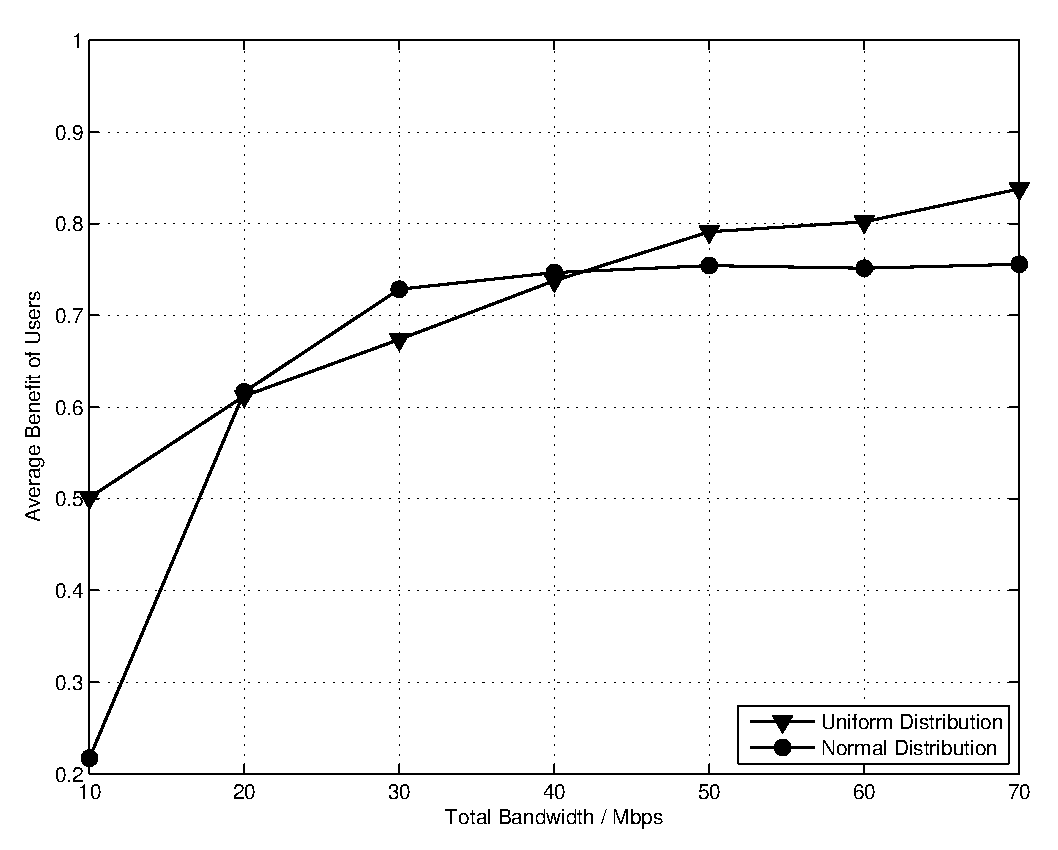
\includegraphics[width = \textwidth]{bayesian_normal_bandwidth_vs_avg_benefit.eps} 
    \caption{用户平均收益} 
    \label{fig:chap_bayesian:normal_bandwidth_vs_avg_benefit} 
  \end{minipage}% 

  \begin{minipage}[t]{0.5\linewidth} 
    \centering 
    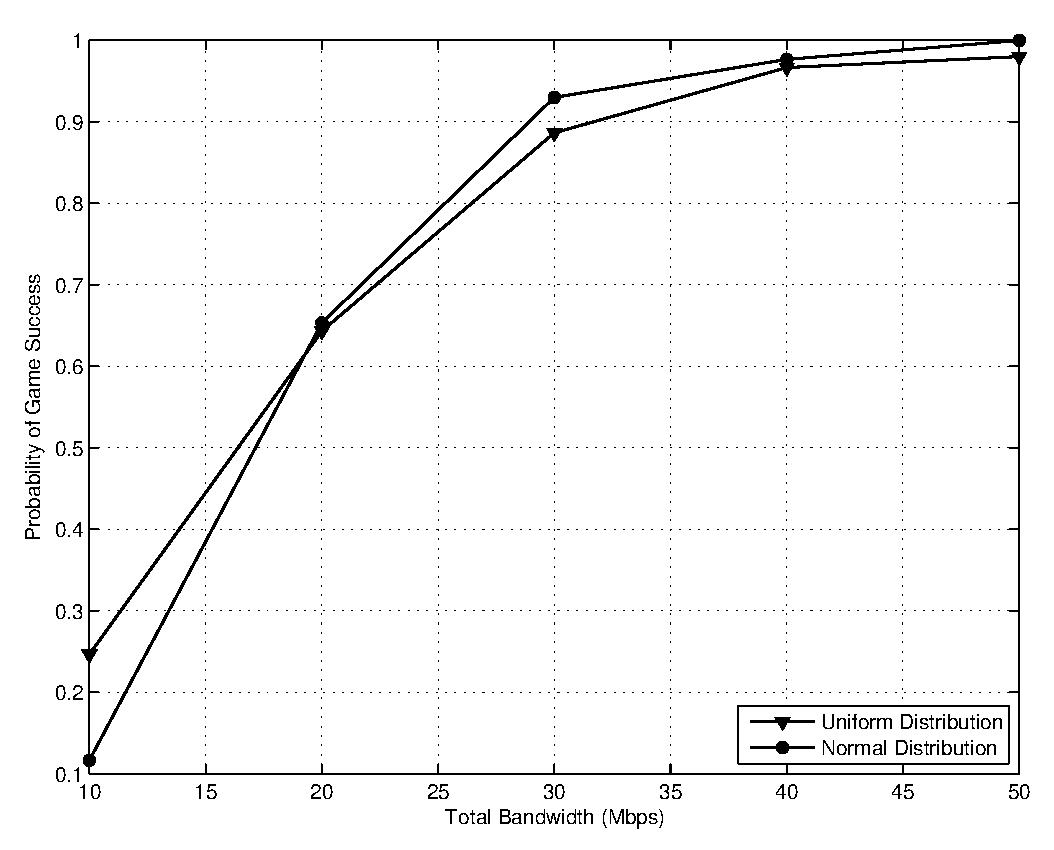
\includegraphics[width=\textwidth]{bayesian_normal_bandwidth_vs_success_probability.eps} 
    \caption{博弈成功概率} 
    \label{fig:chap_bayesian:normal_bandwidth_vs_success_probability} 
  \end{minipage} 
\end{figure}

%%%%%%%%%%%%%%%%%%%%%%%%%%%%%%%%%%%%%%%%%%%%%%%%%%%%%%%%%%%%%%%%%%%%%
%\begin{figure}[tb] 
%    \centering
%  \begin{minipage}[t]{0.5\linewidth} 
%    \centering 
%    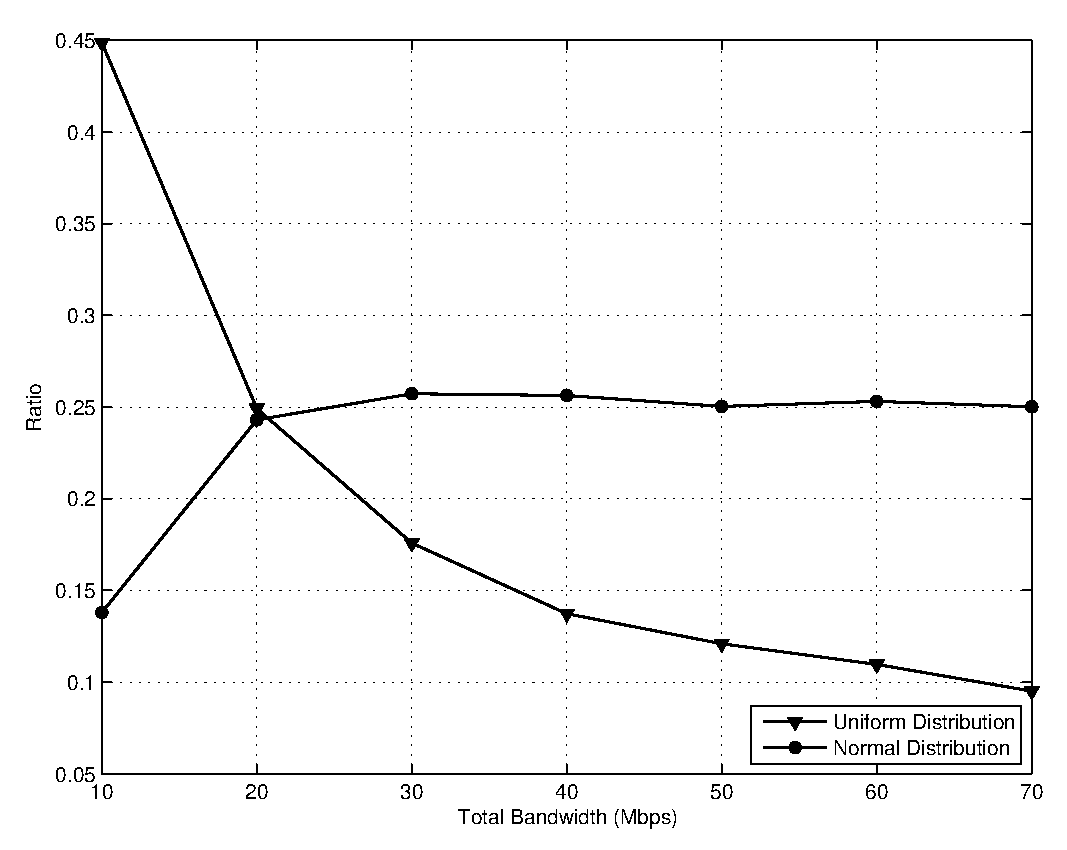
\includegraphics[width=\textwidth]{bayesian_normal_bandwidth_vs_withdraw_bw.eps} 
%    \caption{回收资源占总资源的比率} 
%    \label{fig:chap_bayesian:normal_bandwidth_vs_withdraw_bw} 
%  \end{minipage} 
%\end{figure}
仿真脚本通过改变系统的资源总量,来观察博弈结果的变化情况。
很明显,从\figref{fig:chap_bayesian:normal_bandwidth_vs_user_number}可以看出,资源总量的变化首先影响的是在线用户的数目。
系统总带宽的增多,很自然可以容纳更多用户。
与理论分析相同,单个用户决策“慷慨”的概率降低,\figref{fig:chap_bayesian:normal_bandwidth_vs_generosity}所示;
但同时,我们从
\figref{fig:chap_bayesian:normal_bandwidth_vs_avg_benefit}、
\figref{fig:chap_bayesian:normal_bandwidth_vs_success_probability}中可以看到,
用户的平均收益和一次博弈成功概率都会增多。
这里,“一次博弈成功概率”是指在一次博弈过程中,至少有~$m$~个参与者愿意减少自己占用资源的数量的概率。
用户的数目多少对于博弈的结果影响很大。
从单个用户的角度看,参与者数目增多会使得单个参与者选择“慷慨”的概率下降,
单个参与者从自己的利益出发,更希望其它的参与者选择“慷慨”而自身选择“自私”的情况下还能得到收益。
但是,从集体的角度看,用户数目的增多会弥补这一问题。
这说明,用户数目增多会激发集体的“理性”在更大程度上发挥作用,
在保证在线用户基本满意的前提下使系统本身受益。系统可以收集更多“空闲”资源放入空闲资源池中,供下一次资源分配来使用。
%如\figref{fig:chap_bayesian:normal_bandwidth_vs_withdraw_bw} 所示。
\subsection{仿真实验二}
\esubsection{Simulation Experiment II}
第二个仿真脚本,是对分配算法的一个实例模拟。
一个用户产生器,按照泊松流来模拟产生用户的到达。
其中,到达率为每小时~$300$~个用户。用户在系统中的停留时间服从均值为~$120$~秒的指数分布。
整个仿真时间持续~$2$~个小时。

这个脚本让我们从时间维度上观察所提出的博弈分配算法在一个基站中起的作用。
仿真的结果如 \figref{fig:chap_bayesian:time_vs_ongoing_user_number} 和\figref{fig:chap_bayesian:time_vs_bw_utilization}所示。
每幅仿真结果图中有三条曲线。在基准算法(baseline)中,如果有空闲资源则分配;如果没有则拒绝用户的资源申请。
其它两条曲线分别是采用业务类型分布为正态分布或均匀分布的博弈模型及相应的分配算法。
这里我们仅考察系统用户的容量和资源利用率指标。
系统开始仿真后,大约在~$30$~分钟后,指标进入相对稳定状态并略有波动。
从仿真的结果可以看出,由于在线的用户使用了博弈的分配算法,本质上是将已经分配给用户一部分资源使得用户将其释放出来,
所以空闲资源会得到补充,进而新的用户得以进入系统中。
因此,从用户容量来看,明显博弈分配算法会优于比较算法。
从系统的资源利用率上看,两种博弈的算法略好于基准算法。
%%%%%%%%%%%%%%%%%%%%%%%%%%%%%%%%%%%%%%%%%%%%%%%%%%%%%%%%%%%%%%%%%%%%%
\begin{figure}[!tb] 
   \centering
  \begin{minipage}[t]{0.5\linewidth} 
    \centering 
    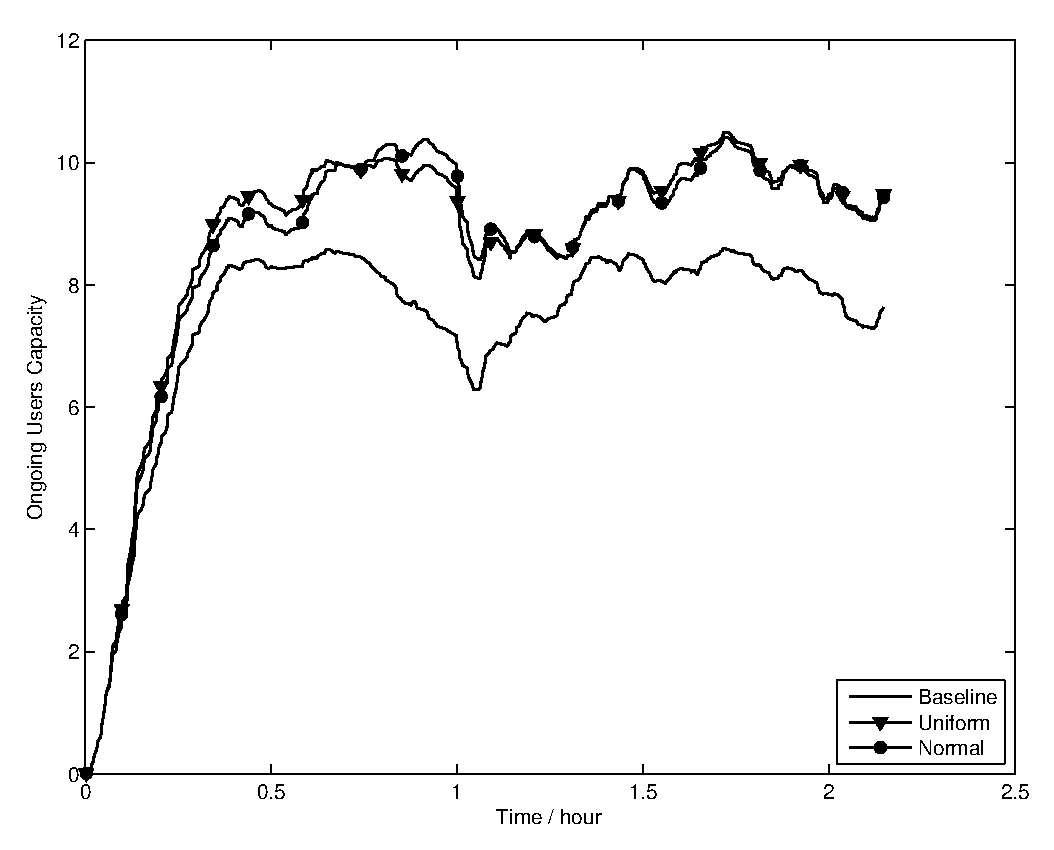
\includegraphics[width=\textwidth]{bayesian_time_vs_ongoing_user_number.eps} 
    \caption{系统在线用户容量} 
    \label{fig:chap_bayesian:time_vs_ongoing_user_number} 
  \end{minipage} 

  \centering
  \begin{minipage}[t]{0.5\linewidth} 
    \centering 
    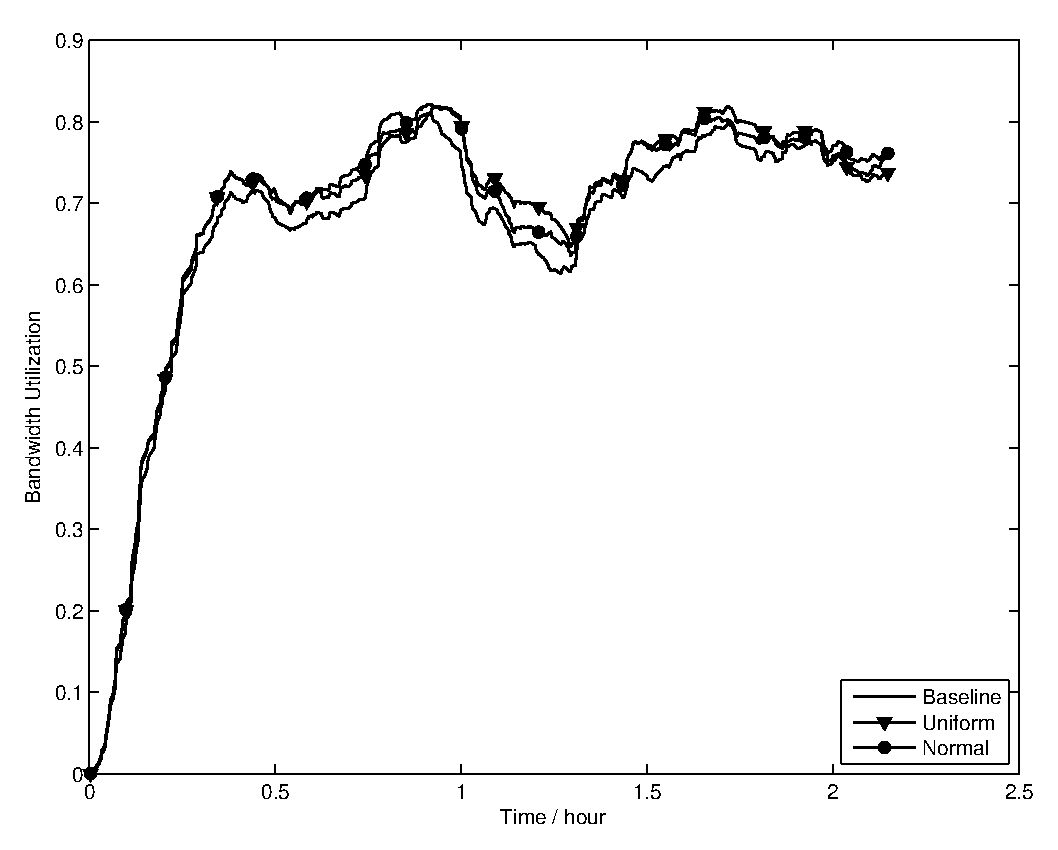
\includegraphics[width=\textwidth]{bayesian_time_vs_bw_utilization.eps} 
    \caption{系统资源利用率} 
    \label{fig:chap_bayesian:time_vs_bw_utilization} 
  \end{minipage} 
\end{figure}
\section{小结}
\esection{Chapter Summary}
本章针对网络中业务逐渐增多的趋势,提出通过概率连续随机变量来描述用户的业务类型。
与传统的离散分类不同,新的方法可以更加细致地刻化用户业务特征。
并且根据网络的实际情况,我们提出在不完备信息的情况下通过构造Bayesian博弈模型的方法来寻求使得所有用户满意的资源分配混合策略。
通过理论的分析与仿真实验证明,所提出的业务描述方法及博弈算法,为有效地解决在多用户竞争下的资源分配问题提供另外一条新的途径。



%
\graphicspath{ {../body/handover_figures/}}
\chapter{高速移动用户的基站切换}
\echapter{Handover or High Velocity Mobile Station}
\label{chap_iccs_handover_alogrithm}
本章研究的内容是
如何改善高速移动用户基站切换成功率的问题。
首先我们以移动WiMAX网络为例,
对移动用户基站切换所涉及到的具体流程与信令进行了细致地分析与讨论。
然后,建立了一个切换信令协议交换的概率模型;
并且针对用户的移动速度对切换成功概率的影响进行了深入地理论分析。
最后提出了一个用于在不同移动速度下保证切换成功率的自适应前向纠错方案。
该算法旨在通过提供增加额外的信令保护措施来确保切换过程满足所需的设计要求。


\section{引言}
\esection{Introduction}
\label{section_iccs_handover_algorithm_introduction}
在蜂窝通信网络中,
术语“切换”(handover, handoff)是指将一个正在通话或是进行数据传输业务的移动用户从一个通信信道转到另一个通信信道的过程。
通常,出现切换过程的原因有多种。
例如,一个正在通信的用户从一个基站(Base Station,BS)进入到了另一个基站的信号覆盖范围,
为了避免通信中断,这个用户就要进行切换操作:
在断开与当前基站或小区连接的同时,连接上第二个基站继续保持通信过程。
还有的时候,用户位于几个基站覆盖域的重叠区域。
此时,如果出现某个基站信号质量比当前服务的基站信号质量好,那么,为了寻求更好的通信质量,
切换过程也会发生。
即使在同一基站有时也会发生切换操作。例如,在某些非CDMA的网络中,
如果一个用户当前使用的信道被邻近小区使用同样信道的用户严重干扰,
那么基站系统也会将此用户的信道切换到同一基站系统的另外一个质量更好的信道上。
还有,如果网络基础架构中存在有宏小区和微小区的设计,在这两种小区之间的信道转变,也称之为切换。
此外,在CMDA网络中,规定一种由于“远近效应”产生的特殊切换过程。
一个用户为避免对其它用户的干扰主动地切换到另一个信道,即使当前通信质量较好。
基站切换可以是在同一网络中的小区切换(也被称为微移动性,Micro-mobility),也可以在异构的网络中的切换。
譬如是无线局域网(WLAN)与3G通信网之间的切换。

本章中所涉及的切换是指用户在移动过程中(从一个地理位置到另一个地理位置,如图\ref{fig:chap_iccs_handover_bs}),用户的通信保持不被中断\cite{Pollini:1996:THD}\cite{Wright:ICMB2007}。

为了能够具体地分析一个基站的切换流程,我们以移动WiMAX的切换协议作为分析的目标。
首先简要介绍一下移动WiMAX网络。
作为3G通信标准之一,WiMAX是一项用于替代现在有线宽带访问技术如ADSL,提供最后一公里的无线网络接入技术。
它提供一种方便快速的方法来建立无线城域网(WMN)。
这项技术可以对高速数据业务如宽带互联网访问,VoIP,IPTV等高速率应用提供底层网络技术支持。
WiMAX技术用来支持在基站与固定、移动或漫游用户终端之间的高速数据连接。
固定WiMAX (IEEE 802.16-2004)的标准中定义了面向连接的媒体访问层(MAC)和基于正交频分复用(OFDM)的物理层协议 \cite{IEEE:802_16D:2005}。
而移动WiMAX(IEEE 802.16e-2005)的标准中还规定了对于移动用户所需的各种MAC层及物理层协议\cite{IEEE:802_16E:2006}。


%%%%%%%%%%%%%%%%%%%%%%%%%%%%%%%%%%%%%%%%%%%%%%%%%%%%%%%%%%%%%%%%%%%%%
\begin{figure}[t]
\begin{centering}
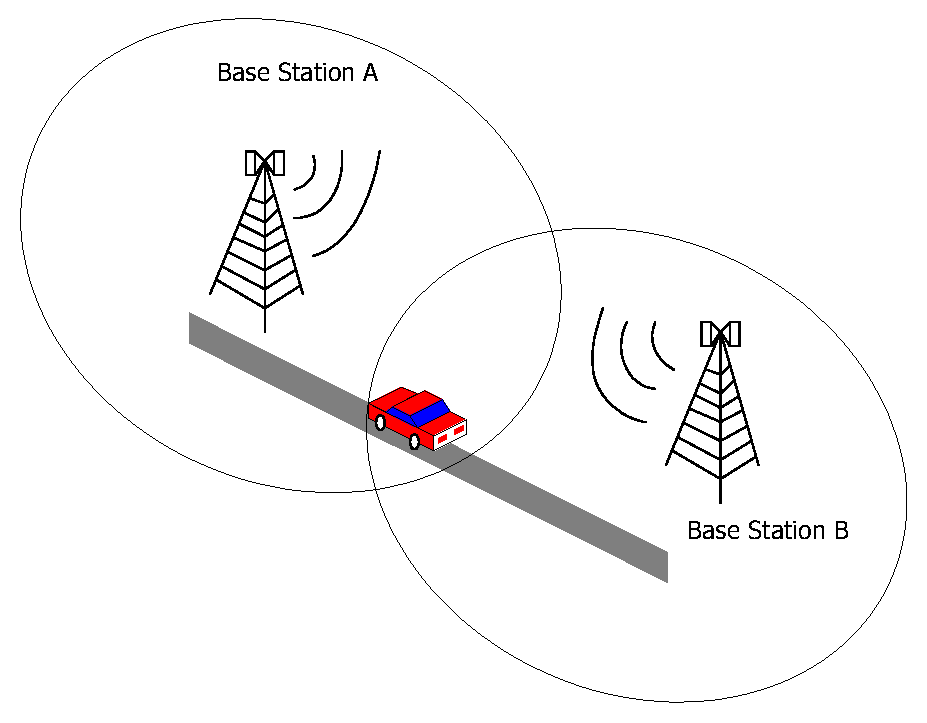
\includegraphics[height=6.75cm]{../figures/iccs_handover_bs}
%\caption{Simulation results of the probability of a handover success using the proposed adaptive FEC scheme.}
\caption{基站切换示意图}
\label{fig:chap_iccs_handover_bs}
\end{centering}
\end{figure}
%%%%%%%%%%%%%%%%%%%%%%%%%%%%%%%%%%%%%%%%%%%%%%%%%%%%%%%%%%%%%%%%%%%%%

当前的移动WiMAX标准详细定义了在切换过程中所需的切换信令协议。
这些协议被用来在单点到多点(Point-to-multipoint,PMP)模式的通信中支持切换过程。
通常,切换技术可以细分成两种:软切换(Soft handover, SHO)和硬切换(Hard Handover,HHO)。
在软切换过程中,移动台在切断与原有基站通信之前,就已经完成和目标基站的切换信令交换过程,并建立了正常的通信连接。
而在硬切换过程中,移动台先要完全断开与原有服务基站的连接,然后再与目标基站建立通信连接。
显然,软切换的优点在于在切换的过程中,数据连接始终存在。
但是同时资源利用率相比硬切换要低。
在硬切换过程中,数据连接会在一个小段时间内断开。
由此引入了一些延时,对于时间敏感的应用而言,需要做专门地处理和优化来确保通信服务质量。
此外,对于时间敏感的应用,软切换也会进行一些优化的处理才能保证在移动WiMAX中QoS。


近些年来,对于软切换方面的研究,许多学者做了大量工作。
一部分人的工作是集中在目标基站的选择策略上。
通过对移动台位置变化的预测、收集分析相邻基站的QoS信息或是对基站信号的分析来优化目标基站的选择\cite{Hsieh:INFOCOM2003}\cite{DooHwan:WPC2006}。
另外一些人的工作主要是集中在提高某些QoS的指标。
例如,学者Minsiki为了解决在切换过程中丢包率增加的问题,采用交叉层的设计方法。他们在上层设备中,如网络层中的路由器,缓存切换用户的数据\cite{MinsikICACT2006}。
Chen等学者为了减少切换过程中的延时,提出了一种预协商的机制。
这个机制利用预测移动台与基站间的距离,提前在目标基站中分配所需要的资源\cite{JenHui:AUSWIRELESS:2007}。
学者Ling通过用IP层的链路来传送MAC层的信息来达到减少切换延时的目的\cite{LingVTC2007}。
还有一些学者的研究集中在切换过程中出现的CID(Connection Identifier) 分配冲突,提出了更为合理的分配方案,或是对移动台的数据进行分类处理,最终也可以提高QoS的水平\cite{Hu:TVT2004}\cite{Wenhua:ICC2007}。


以往的大部分工作主要是从数据链路层或IP层来考虑切换的性能。他们的工作一般是假设无线信道是一个理想信道。在本章中,我们认为如果物理层的信道工作能与数据链路层工作进行协调,就可以有效提高切换性能。特别是在移动台高速运动的状态下。
下面,我们将会分析信道质量对切换信令交换流程的影响。
然后,通过建立信令交换的概率模型来分析在高速移动状态时的切换性能。
最后通过建立一个简单实用的自适应前向纠错方法来提高切换的成功率和效率。


\section{基站切换成功概率模型}
\label{section_iccs_handover_algorithm_mobility_analysis}
\esection{Probability Model of Handover}
切换的性能与效率通常可以用一个切换的成功率来描述。我们通过统计在切换过程中每次信令的交换成功概率来计算出完成整个切换过程概率。
在高速运动的切换过程中,移动速度会对切换造成非常大的影响。它不但反映移动台切换延时情况,也在研究切换用户丢包模型中扮演着重要的角色。
\subsection{切换的流程建模分析}
\esubsection{Hanover Protocols in WiMAX}
\label{subsection_iccs_handover_algorithm_mobility_analysis_handover_flow}
在IEEE 802.16e的标准中,切换信令的交换流程如图\ref{fig:chap_iccs_handover_algorithm_handover_flow}所示。
基站会周期地广播“邻近通告消息”(Neighbor Advertisement Message, MOB\_NBR-ADV)。
这个消息用来标识邻近基站或是它们的信道特征。
移动台总是会侦听此消息来收集邻近基站的信息。
如果一个移动台检测到与当前服务基站的信道变差,它会发送一个请求消息(MOB\_SCAN-REQ)给当前服务的基站。
如果基站收到此请求消息后,会反馈给移动台一个消息(MOB\_SCAN-RSP)。
此消息会指示移动台使用特定的无线资源(如时隙)来进行扫描操作(Scanning),确定目标基站。
当扫描操作结束后,移动台初始化切换过程,发送切换请求消息(MOB\_MSHO-REQ)给当前基站。
然后基站会发送响应消息信令(MOB\_BSHO-RSP)。
当移动台收到此消息时,它会发送消息(MOB\_HO-IND)通知当前基站可以关闭此移动的连接,释放无线资源。
(如果是硬切换,移动台会中断与当前服务基站的连接。如果是软切换,连接会继续保留直到与目标基站的信令交换结束。)
最后,移动台与目标基站交换测距消息以及重新接入的各种信令来完成剩余的切换流程。
综合上述的描述,一次成功的切换过程,尽管无线资源的分配也是切换需要考虑的内容,
但从数据链路层的信令层面上看,其核心首先是各种切换信令的成功传递与交换。

%%%%%%%%%%%%%%%%%%%%%%%%%%%%%%%%%%%%%%%%%%%%%%%%%%%%%%%%%%%%%%%%%%%
\begin{figure}[t]
\centering
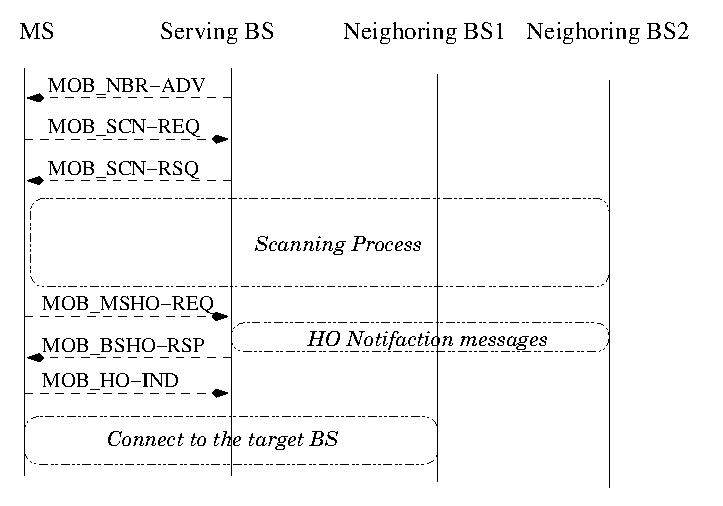
\includegraphics[height=7.75cm]{iccs_handover}
\caption{切换流程示意图}
%\caption{Illustration of the handover procedure.}
\label{fig:chap_iccs_handover_algorithm_handover_flow}
\end{figure}
%%%%%%%%%%%%%%%%%%%%%%%%%%%%%%%%%%%%%%%%%%%%%%%%%%%%%%%%%%%%%%%%%%%

\subsection{切换成功概率建模与误比特率}
\esubsection{Probability of Handover Success and Bit Error Rate}
根据上面的分析,我们考虑一个这样的切换过程模型。
不失一般性,我们假设在一次移动台的切换过程中有~$M$~($M \ge 2 $)个信令需要交换。
设事件~$A_i$~表示一次信令的传送。
 ~$p_i$~是此次信令成功传送的概率,其中 ~$i = 0,1, \cdots, M-1 $~。
如果不考虑自动重传(ARQ)的策略,则有以下结论:
%%%%%%%%%%%%%%%%%%%%%%%%
\begin{equation}
\label{eq:chap_iccs_handover_algorithm_pro_mess_no_tran}
\begin{cases}
P(A_{i})=p_{i}\\
P(\bar{A}_{i})=1- p_{i}
\end{cases}
\end{equation}
%%%%%%%%%%%%%%%%%%%%%%%%
其中,~$i=0,1,\cdots,M-1$~。
接下来我们分析一下有重传策略的情况。
在切换过程中,重传策略不但可以用于用户数据的传递,也可用于保证信令消息的可靠传送。
所以,根据切换信令的要求,这里我们假设一个信令消息如果不能被对方成功接收,将会被重传定时器激发重新发送过程,并直到接到对方反馈为止。
那么,如果考虑了重传策略后,则公式 (\ref{eq:chap_iccs_handover_algorithm_pro_mess_no_tran})可以重新写为下面的式子:
%%%%%%%%%%%%%%%%%%%%%%%%
\begin{equation}
\label{eq:chap_iccs_handover_algorithm_Pro_basic01}
P(A_{i})=\sum_{j=1}^{N_{i}}q_{i}^{j-1}p_{i}=\sum_{j=1}^{N_{i}}
(1-p_{i})^{j-1}p_{i},\quad N_{i}\geq1,
\end{equation}
%%%%%%%%%%%%%%%%%%%%%%%%
其中,~$N_i$~表示在一次切换过程中,第~$i$~个信令消息在成功接收前被传递的次数。在切换过程中有~$M$~个信令消息,那么,只有~$M$~个信令都成功收到,切换才认为是成功的,所以切换成功的概率可表示为:
%%%%%%%%%%%%%%%%%%%%%%%%%%
\begin{equation}
\label{eq:chap_iccs_handover_algorithm_Pro_basic02}
P_{succ}=\prod_{i=0}^{M-1}P(A_{i})=\prod_{i=0}^{M-1}
\left[\sum_{j=1}^{N_{i}}(1-p_{i})^{j-1}p_{i}\right].
\end{equation}
%%%%%%%%%%%%%%%%%%%%%%%%%%
因为当前通信系统的物理层中普遍采用交织信道编码的技术,所以模型中的无线信道可以假设为无记忆的信道。那么,概率~$p_i$~将主要与移动台和基站之间的无线信道的误比特率有关。我们用数学公式表示如下:
%%%%%%%%%%%%%%%%%%%%%%%%%%
$$
p_{i}=\varphi(P_{b}(\gamma_{b}),\: L_{i}),
$$
%%%%%%%%%%%%%%%%%%%%%%%%%%
其中,~$P_b(\gamma_b)$~是当接收比特信噪比为~$\gamma_b$~的误比特概率。这样,如果设第~$i$~个信令消息的长度为~$Li$~,则有
%%%%%%%%%%%%%%%%%%%%%%%%
\begin{equation}\label{eq:chap_iccs_handover_algorithm_Pro_basic03}
p_{i}=[1-P_{b}(\gamma_{b})]^{L_{i}}.
\end{equation}
%%%%%%%%%%%%%%%%%%%%%%%%
所以,将公式(\ref{eq:chap_iccs_handover_algorithm_Pro_basic03})代入公式(\ref{eq:chap_iccs_handover_algorithm_Pro_basic02}),可以得到切换模型中的切换成功概率与无线信道误比特率之间的关系。
%%%%%%%%%%%%%%%%%%%%%%%%%
\begin{align}
\label{eq:chap_iccs_handover_algorithm_Pro_basic_final}
\notag P_{succ}&=\prod_{i=0}^{M-1}P(A_{i})\\
&=\prod_{i=0}^{M-1}\left\{ \sum_{j=1}^{N_{i}}\left\{ 1-[1-P_{b}(\gamma_{b})]^{L_{i}}\right\} ^{j-1} \cdot[1-P_{b}(\gamma_{b})]^{L_{i}}\right\}
\end{align}
%%%%%%%%%%%%%%%%%%%%%%%%%%
%%%%%%%%%%%%%%%%%%%%%%%%%%%%%%%%%%%%%%%%%%%%%%%%%%%%%%%%%%%%%%%%%%%%%
\begin{figure}[t]
\begin{centering}
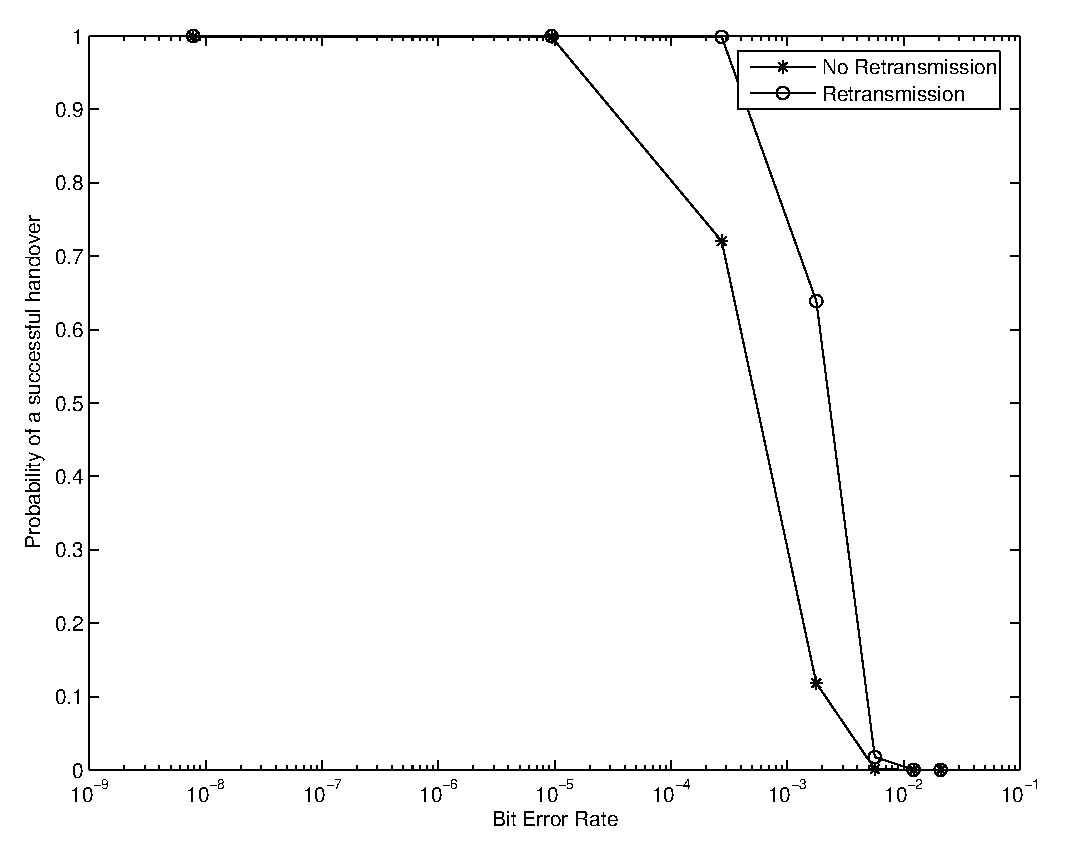
\includegraphics[height=7.75cm]{iccs_ber_prob}
\par\end{centering}
%%\caption{Probability of a handover success as a function of BER, where ~$M=5,\sum_{i=0}^{M-1}N_i<=50,L_i=250$~ bits in this case.}
\caption{切换成功概率与误比特率的关系。在此例中,~$M=5,\sum_{i=0}^{M-1}N_i<=50,L_i=250$~}
\label{fig:chap_iccs_handover_algorithm_PBER}
\end{figure}
%%%%%%%%%%%%%%%%%%%%%%%%%%%%%%%%%%%%%%%%%%%%%%%%%%%%%%%%%%%%%%%%%%%%%
这里,我们给出公式(\ref{eq:chap_iccs_handover_algorithm_Pro_basic_final})的一个例子,如图 \ref{fig:chap_iccs_handover_algorithm_PBER} 所示。
可以明显地看出,对于固定的~$N_i$~,切换的成功概率~$P_{succ}$~随着误比特概率~$P_b(\gamma_b)$~的增大而降低。当误比特率较大时(在~$10^{-4}$~到~$10^{-2}$~之间),使用重传策略会有效地改善切换的成功率。

\subsection{切换成功概率模型与移动台速度}
\esubsection{Probability of Handover Success and Velocity of MS}
上一节的分析指出了切换成功概率与两个重要的参数有关:一是信道的误比特率,二是信令消息的重传次数。
在一个实际的WiMAX网络中,这二者都与移动台的移动速度有关。
首先,移动的速度会影响多谱勒频率偏移,进而影响信道的误比特率,最终对信令消息的重传次数产生影响。
其次,两个相邻基站覆盖的交叠部分的物理距离有限,因而不能做到无限制的重传。
所以,一个快速移动的终端要求基站切换的速度与时间也有更严格的要求。
基于上述的考虑可知,通常情况下,移动台的移动速度越快,切换成功的概率会越低。

为了定量的分析起见,我们假设在切换过程中,对信令处理的时间可以忽略不计的。
所以,在整个切换过程中的延时可以写为下面的式子,
%%%%%%%%%%%%%%%%%%%%%%%%%%%%%%%%%%%%%
$$
T_{M}=(N_{0}+N_{1}+\cdots+N_{M-1})\cdot T_{retx}+M\cdot T_{prop},
$$
%%%%%%%%%%%%%%%%%%%%%%%%%%%%%%%%%%%%%
其中,~$N_i$~表示第~$i$~个信令传递的次数。~$T_{retx}$~是同一信令消息重传的计时器间隔,~$T_{prop}$~是在移动台与基站之间的承载信令的电磁波传播所需时间。

我们用~$D_{overlap}$~表示在移动台移动方向上两个相邻基站覆盖范围重叠部分的距离。
如图\ref{fig:chap_iccs_handover_bs}如示。
$v_m$是移动台的移动速度。
因此,在一次成功的基站切换过程中,需要满足下面的时间约束\eqref{eqn:chap_handover:times_T_M}:
%%%%%%%%%%%%%%%%%%%%%%%%%%%%%%%%
\begin{equation}
T_{M}<\frac{D_{overlap}}{v_{m}}.
\label{eqn:chap_handover:times_T_M}
\end{equation}
%%%%%%%%%%%%%%%%%%%%%%%%%%%%%%%
在这个约束下,一次成功切换的概率可以进一步被改写\eqref{eq:chap_iccs_handover_algorithm_Pro_basic_final00},

%%%%%%%%%%%%%%%%%%%%%%%
\begin{equation}
P_{succ}=\left\{
\begin{array}{ll}
\prod_{i=0}^{M-1}\left[\sum_{j=1}^{N_{i}}(1-p_{i})^{j-1}p_{i}\right],
& \mbox{if }T_{M}<\frac{D_{overlap}}{v_{m}},\\
\\0, & \mbox{others},
\end{array}\right.\label{eq:chap_iccs_handover_algorithm_Pro_basic_final00}
\end{equation}
%%%%%%%%%%%%%%%%%%%%%%%
其中,
%%%%%%%%%%%%%%%%%%%%%%%%
\begin{align*}
T_{M}=\sum_{i=0}^{M-1}(N_{i})\cdot T_{retx}+M\cdot T_{prop} \\
p_{i}=[1-P_{b}(\gamma_{b})]^{L_{i}}
\end{align*}
%%%%%%%%%%%%%%%%%%%%%%%%
这里,假设使用Rayleigh信道。平均接收符号的信噪比(energy-to-noise)可以表示为:\cite{GLST:PMC2002}\cite{Leung:WCNC2005}
%%%%%%%%%%%%%%%%%%%%%%%%
\begin{equation}
\bar{\gamma}_{s}=\frac{1}{1-\frac{1}{N^{2}}\left[N+2\sum_{i=1}^{N-1}\left(N-i\right)J_{0}(2\pi f_{m}T_{s}i) \right]
+\frac{NT_{s}}{E_s/N_{0}}},
\end{equation}
%%%%%%%%%%%%%%%%%%%%%%%
其中,~$N$~是OFDM子载波的个数,~$T_s$~是一个K阶QAM调制的符号在一个子载波上的传输时间。~$N_0$~是噪声功率, ~$E_s$~是传送每个符号的平均能量。~$f_{m}=fv_{m}/c $~是最大的多谱勒频偏,~$f$~为载波频率,~$v_m$~为移动台的速度,~$c$~为光速。那么相应的接收到的平均比特信噪比为
%%%%%%%%%%%%%%%%%%%%%%%%
\begin{align}
\bar{\gamma}_{b}&= \frac{ \bar{\gamma}_s} {\log_2K} \notag\\
&=\frac{1/\log_{2}K}{1-\frac{1}{N^{2}}\left[N+2\cdot \sum_{i=1}^{N-1}\left(N-i\right) J_{0}(2\pi f_{m}T_{s}i) \right]
+\frac{NT_{s}}{\log_{2}K}\left(\frac{1}{E_{b}/N_{0}}\right)}
\label{eqn:chap_handover:avg_snr}
\end{align}
其中,
\begin{equation*}
J_{0}(2\pi f_{m}T_{s}i) = \frac{1}{\pi}\int_0^\pi \cos(2\pi f_m T_{s}i \sin \theta) d \theta
\end{equation*}
%%%%%%%%%%%%%%%%%%%%%%%
此处,我们假设以Clarke-Jakes的模型为基础的Rayleigh信道模型。

%其中,~$Y$~定义为
%%%%%%%%%%%%%%%%%%%%%%%%
%$$
%Y=\sum_{i=1}^{N-1}\left(N-i\right)J_{0}(2\pi f_{m}T_{s}i)
%$$
%%%%%%%%%%%%%%%%%%%%%%%%%
对于K阶的QAM调试(如果~$K=4$~,调制的方式是QPSK;如果~$K=16$~,那么就是16-QAM)。
我们假设在接收端可以进行出错的符号检测。那么对于当接收比特能量与噪声比为~$\gamma_b$~时,误比特概率(bit error, BER)为~$P_b(\gamma_b)$~可以写为:
%%%%%%%%%%%%%%%%%%%%%%%
\[
{{P}_{b}}=\int\limits_{0}^{\infty }{{{P}_{b}}(\gamma ){{f}_{{{\gamma }_{b}}}}(}\gamma )d\gamma
\]
%%%%%%%%%%%%%%%%%%%%%%%%
其中,~$f_{\gamma_b}$~是Rayleigh信道模型的比特能量与噪声比的概率密度函数。它定义如下:
%%%%%%%%%%%%%%%%%%%%%%%%%
\[{{f}_{{{\gamma }_{b}}}}(\gamma )=\frac{\exp (\frac{-\gamma }{{{{\bar{\gamma }}}_{b}}})}{{{{\bar{\gamma }}}_{b}}},\gamma \ge 0\]
%%%%%%%%%%%%%%%%%%%%%%%%%%%%
我们假设载波间的干扰(ICI)为高斯白噪声。这个值近似在~$256 \le N \le 1024$~是比较精确的\cite{Leung:WCNC2005}。那么,对于K阶的QAM和Gray码,可以有如下的近似,
%%%%%%%%%%%%%%%%%%%%%%%
\begin{equation}
P_b(\gamma_b) \approx \frac{P_M(\gamma_s)}{\log_2 K}
\end{equation}
%%%%%%%%%%%%%%%%%%%%%%%
其中,~$P_K$~是符号的错误概率。特别对于QPSK,有
%%%%%%%%%%%%%%%%%%%%%%%%
\begin{align}
\label{eq:chap_iccs_handover_algorithm_BER_V}
P_{b}(\gamma_{b})&= Q\left(\sqrt{2\gamma_{b}}\right).\\
Q(x) &= \int^x_{-\infty} \frac{1}{\sqrt{2\pi}}e^{-y^2/2}dy \notag
\end{align}
%%%%%%%%%%%%%%%%%%%%%%%%
把公式(\ref{eq:chap_iccs_handover_algorithm_Pro_basic_final00})和公式( \ref{eq:chap_iccs_handover_algorithm_BER_V})合并则有下面的结果。
%%%%%%%%%%%%%%%%%%%%%%%
\begin{equation}
P_{succ}=\left\{
\begin{array}{ll}
\prod_{i=0}^{M-1}\left[\sum_{j=1}^{N_{i}}(1-Q\left(\sqrt{2\gamma_{b}}\right))^{j-1}Q\left(\sqrt{2\gamma_{b}}\right)\right],
& \mbox{if }T_{M}<\frac{D_{overlap}}{v_{m}},\\
\\0, & \mbox{others}
\end{array}\right.\label{eq:chap_handover:velocity_bit_error_rate}
\end{equation}
其中,~$\gamma_b$~是移动速度的一个函数。
至此,我们可以得到以移动台速度为变量的一个切换成功概率函数模型。其函数图形,如图\ref{fig:chap_iccs_handover_algorithm_Pro_V} 所示。
%%%%%%%%%%%%%%%%%%%%%%%%%%%%%%%%%%%%%%%%%%%%%%%%%%%%%%%%%%%%%%%%%%%%
\begin{figure}[t]
\begin{centering}
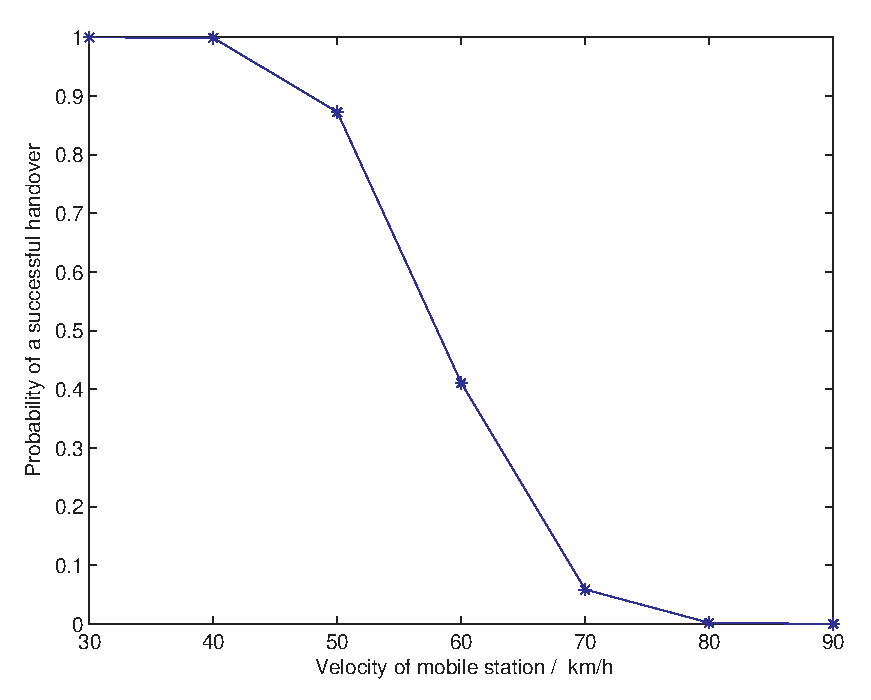
\includegraphics[height=7.75cm]{iccs_speed_prob_theroy}
%%\caption{The probability of a handover success as a function of MS's velocity, where ~$M=5, \sum_{i=0}^{M-1}N_i=50, L_i=250$~ bits in this case.}
\caption{切换成功概率与用户的移动速度关系,在本例中~$M=5, \sum_{i=0}^{M-1}N_i=50, L_i=250$~}
\label{fig:chap_iccs_handover_algorithm_Pro_V}
\end{centering}
\end{figure}
%%%%%%%%%%%%%%%%%%%%%%%%%%%%%%%%%%%%%%%%%%%%%%%%%%%%%%%%%%%%%%%%%%%%

从图中可明显看出,随着移动的速度增快,切换成功概率会显著下降。这样会极大地影响了切换的过程。所以说,如果在高速移动状态下,切换对于移动台来说需要额外的处理。

\section{基于切换成功概率模型的切换方案}
\esection{Handover Scheme with High Velocity MS}
在高速移动状态下,为了提高移动台的切换成功概率,除了可以减小重传间隔、增加重传的次数以外,我们也需要建立更加可靠的通信链路的传输机制来传送信令消息。
本节我们讨论了前向纠错编码的特点,并采用此技术来改善传输的误码率。
前向纠错编码是通过发送端使用冗余比特数来提供差错保护。
这些额外的冗余比特可以帮助接收端检测并纠正错误。
如果采用了前向纠错的技术,数据重传的次数也会降低。
根据WiMAX的标准,切换信令的消息大小约为50到180个字节左右。

不同的前向纠错编码方案可以提供不同的纠错能力。
对于同一种前向纠错码而言,冗余比特数越多,纠错能力也超强。
同时由于无线信道的限制及交换的信令消息较多,所以要在满足设计要求的基础上尽可能减少冗余比特数。

因此,下面我们定量地讨论冗余比特的个数。对于一个给定的移动台速度,我们要能基于系统设计要求达到的切换成功率来计算出冗余比特数。为了简单起见,我们使用切换消息信令的平均长度,设切换消息传输一次的成功的概率为~$\tilde{p}$~以替换公式(\ref{eq:chap_iccs_handover_algorithm_Pro_basic_final00})中的~$p_i$~,如下
%%%%%%%%%%%%%%%%%%%%%%%%%%%%%%%%%%%
\begin{align}
\notag P_{succ} &= \prod_{i=0}^{M-1}P(A_{i})\\
&= \prod_{i=0}^{M-1}\left[\sum_{j=1}^{N_{i}}(1-p_{i})^{j-1}p_{i}\right]\\
\notag &\thickapprox\sum_{i=M}^{S}{i-1 \choose M-1}\cdot\widetilde{p}^{M}(1-\widetilde{p})^{i-M}
\end{align}
%%%%%%%%%%%%%%%%%%%%%%%%%%%%%%%%%%
其中,~$S=\sum_{i=0}^{M-1}N_{i}$~是总共重传的次数。根据前面小节的分析,可以得到如下的公式:
%%%%%%%%%%%%%%%%%%%%%%%%%%%%%%%%%%
\begin{align*}
S & = \sum_{i=0}^{M-1}N_{i}\\
  & = \left\lfloor \frac{(\frac{D_{overlap}}{v_{m}}-MT_{prop})}
        {T_{retx}}\right\rfloor \leq\frac{(\frac{D_{overlap}}{v_{m}}
        -MT_{prop})}{T_{retx}}.
\end{align*}
%%%%%%%%%%%%%%%%%%%%%%%%%%%%%%%%%%
这样,我们就可根据相邻基站覆盖交叠的距离~$D_{overlap}$~和移动台的速度~$v_m$~,得到参数~$S$~;并根据系统设计要求的~$P_{succ}$~进一步计算得每一个信令的成功传输的概率值。如果使用Reed-Solomon(R-S)纠错编码,我们可以推导出如下\eqref{eq:chap_iccs_handover_algorithm_FEC_Pro_final}。
%%%%%%%%%%%%%%%%%%%%%%%%%%%%%
\begin{equation}\label{eq:chap_iccs_handover_algorithm_FEC_Pro_final}
\tilde{p}\approx\frac{2^{k-1}}{k(2^{k}-1)^{2}}\sum_{j=t+1}^{2^{k}-1}j
\cdot{2^{k}-1\choose j}_{}^{}\cdot p^{j}(1-p)^{2^{k}-1-j},
\end{equation}
%%%%%%%%%%%%%%%%%%%%%%%%%%%%%
其中, ~$t=\lfloor\frac{N-k}{2}\rfloor$~ 是编码的符号纠错能力,~$N$~是全部的比特数,~$k$~是信令消息的比特数, ~$\lfloor{x}\rfloor$~表示不超过~$x$~的最大整数。那么冗余比特数~$N-k$~可以确定下来。图 \ref{fig:chap_iccs_handover_algorithm_AFEC_bits} 表明了在切换流程要达到不同的切换成功概率(~$50\%,80\%,99\%$~)下,在不同的速度下,移动台切换所需的冗余比特数。
%%%%%%%%%%%%%%%%%%%%%%%%%%%%%%%%%%%%%%%%%%%%%%%%%%%%%%%%%%%%%%%%%%%%%%%%%%%
\begin{figure}[t]
\begin{centering}
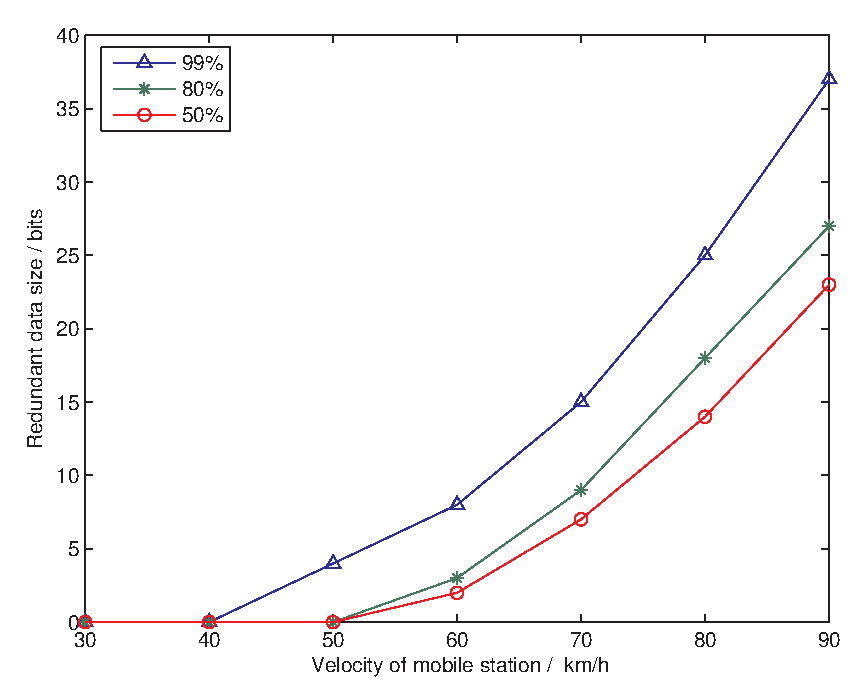
\includegraphics[height=6.75cm]{iccs_speed_size_theory}
\caption{RS码中的冗余比特数与移动台速度之间的关系,其中,假设~$k=250$~比特}
\label{fig:chap_iccs_handover_algorithm_AFEC_bits}
\end{centering}
\end{figure}
%%%%%%%%%%%%%%%%%%%%%%%%%%%%%%%%%%%%%%%%%%%%%%%%%%%%%%%%%%%%%%%%%%%%%%%%%%%

如图 \ref{fig:chap_iccs_handover_algorithm_AFEC_bits}所示,当移动台的速度越快,那么为了达到系统设定的切换成功概率,所需的冗余比特数也越多。例如,为了能够达到~$80\%$~的成功概率,如果移动台的速度分别是50,70, 90 km/h,那么所需的冗余比特数是2,10,28。通过上面的分析,我们可以使用一种自适应的方法根据不同的移动台速度来增加所需的冗余比特。

\section{仿真实验与结果分析}
\esection{Simuation and Results}
我们通过计算机仿真实验来验证和评估我们的切换概率模型及相应的前向纠错方案。在实验中,我们使用了NS-2仿真模拟器和修改了的NIST的WiMAX仿真代码\cite{NS2_simulator}\cite{NIST_WIMAX}。实验主要的实验设置参数如表格\ref{chap_iccs_table_I} 所示。

%%%%%%%%%%%%%%%%%%%%%%%%%%%%%%%%%%%%%%%%%%%%%%%%%%%%%%%%%%%%%%%%%%%%%
\begin{table}[htbp]
\wuhao
\centering
%\begin{centering}
\caption{仿真实验的主要参数配置}\label{chap_iccs_table_I}
\begin{tabular*}{0.99\textwidth}{p{7cm} p{7cm}} 
\toprule 
参数名称  & 参数值 \\
\midrule
移动方向上的交叠距离  & 200 米\tabularnewline 
带宽  & 5 MHz\tabularnewline 
载波频率  & 2.5 GHz\tabularnewline 
FFT   & 512\tabularnewline
信道类型  & Rayleigh channel\tabularnewline 
FEC  & Reed-Solomon code\tabularnewline 
移动速度  & 30-90 km/h\\
\bottomrule
\end{tabular*}
%\end{centering}
\end{table}
%%%%%%%%%%%%%%%%%%%%%%%%%%%%%%%%%%%%%%%%%%%%%%%%%%%%%%%%%%%%%%%%%%%%%

这里,我们采用的是自适应的前向纠错码方案。
冗余比特数是理论计算事先得到的。
在切换成功概率为50\%,80\%,99\%的情况下,计算出所需要的冗余比特数。
对于每一组实验参数,仿真进行100次,然后取结果的平均值来得到最后的统计结果。
最终得到的仿真实验结果,如\figref{fig:chap_iccs_results}所示。
从图中我们可以看到,在移动台的速度较低时,少量增加一些冗余比特会使得切换成功的概率会显著增加,并接近于~1。
而当速度逐渐增大后,对于目标为50\%的曲线,切换成功率会下降,但仍然会保持在50\%以上。
这说明,在保证高切换成功率,如99\%,所增加的冗余比特数较多,我们的方案略显些保守。
而且我们也注意到,在速度为70km/h时,理论成功率50\%的曲线存在一个局部极值点。
经过反复实验与比对,我们认为有两个原因会造成:
一是,在NS2系统中的Rayleigh信道模型计算误比特数时存在偏差。
二是,\eqref{eqn:chap_handover:avg_snr}中速度与SNR关系偏差所致。

%%%%%%%%%%%%%%%%%%%%%%%%%%%%%%%%%%%%%%%%%%%%%%%%%%%%%%%%%%%%%%%%%%%%%
\begin{figure}[t]
\begin{centering}
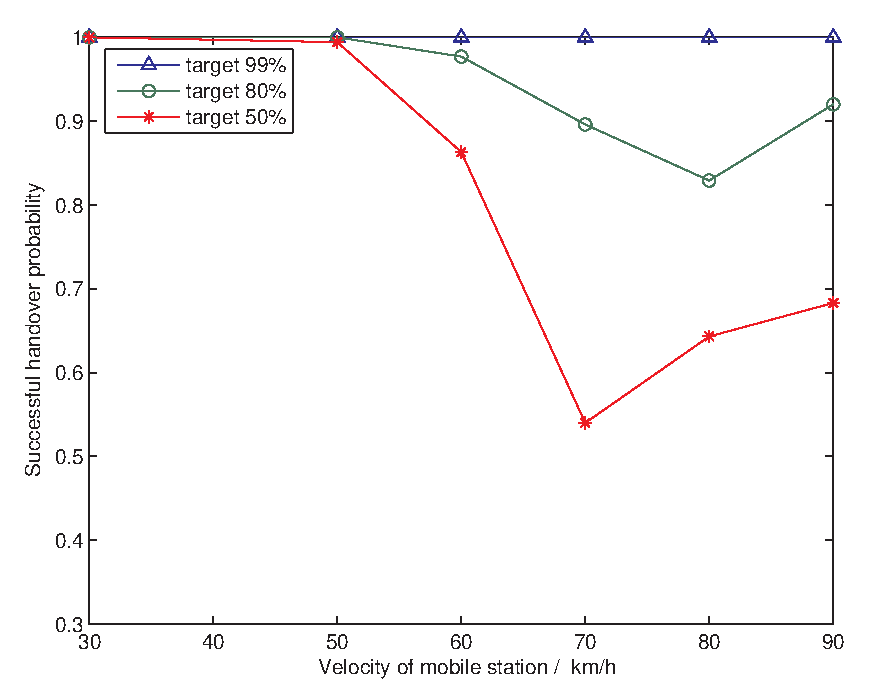
\includegraphics[height=7.75cm]{iccs_speed_prob_simu}
%\caption{Simulation results of the probability of a handover success using the proposed adaptive FEC scheme.}
\caption{仿真实验的结果}
\label{fig:chap_iccs_results}
\end{centering}
\end{figure}
%%%%%%%%%%%%%%%%%%%%%%%%%%%%%%%%%%%%%%%%%%%%%%%%%%%%%%%%%%%%%%%%%%%%%

\section{本章小结}
\esection{Chapter Summary}
在本章中,我们以WiMAX网络为例分析了移动台的移动速度对切换成功率的影响。分析的结果表明,由于移动台的速度增加会导致无线传输的信道变差,进而使得切换信令不能正常收发。又由于切换操作是时间受限的,所以在设计切换时要两方面同时考虑。根据理论分析,我们提出了一个简单有效的自适应前向纠错方案,通过理论计算就可以得到在不同速度下所需的冗余比特数,可以满足在不同移动速度下的切换设计需求。最后仿真实验验证了我们的理论模型和所提出的前向纠错方案的正确性。
%chapter_end

%
%chapter_begin
\chapter{结论与展望}
\echapter{Conclusions and Future Work}
\label{chap_conclusions}
\section{论文总结}
\esection{Conclusions}
互联网技术的发展为多媒体业务的开展提供了广阔的应用平台。
各种新型的互联网应用,也改变了人们对传统互联网通信的认识。这些应用也使得人们希望能始终保持与互联网连接,随时随地得进行自由的信息传递。但是,由于空中接口频谱资源的稀缺,使得无线互联网技术遇到了许多技术难题。

本论文以无线资源管理为主线,以解决数据链路层中所涉及移动性管理和资源的合理公平利用为目标,
针对高速无线移动终端的基站切换问题、基于业务流量特征的呼叫接纳控制算法与资源分配问题,以及博弈论在资源管理方面的应用做了一些有意义的探索。
主要的内容简要总结为如下四点:

\begin{enumerate}[(1.)]
\item
针对多媒体业务用户的呼叫接纳控制与资源管理问题,
我们首先分析了多媒体业务的特点,
建立了一个网络高层服务质量评估与数据链路层质量评估关系的映射模型。
该模型可以针对不同的业务数据流在数据链路层上映射为一个归一化的QoS水平评估指标。
基于这样一个QoS的映射模型,可以有效地评测各个用户连接的QoS水平与资源的需求,并最终提供给呼叫接纳控制单元做为接入控制的判断依据。
而后,所提出的接纳控制算法充分利用了这一模型特点,有效地改善接纳控制的性能。
仿真结果表明,此算法在保证用户服务质量的同时,改善了系统的连接容量、资源利用率、以及新用户的阻塞率。
\item 针对多用户资源竞争的问题,将非对称纳什议价博弈理论引入资源分配问题的解决方案中来。
构造了一个新的资源分配议价博弈模型,定义了博弈参与者的效用,用户的分歧点等。
通过对模型的理论分析,证明了该分配模型满足纳什议价公理所提出的各项约束。
然后,分析了用户议价能力对分配结果的影响,
进而提出以用户应用特征参数值为基础的议价能力的具体定义。
仿真结果表明,所提出的博弈模型与相应的资源分配算法,可以有效地且公平地解决用户资源竞争的问题。所提出的资源分配算法在保证系统资源利用率的同时,也兼顾了各个不同类别用户之间的需求。

\item 研究了在非完备信息下的资源分配Bayesian博弈问题。
针对信息不完整,我们提出一个新的业务类型概率描述方法。此方法不再使用传统的离散的业务描述方式,而是使用连续的概率随机变量的描述方式。。
基于这种描述方式的转变,我们提出并构造了一个基于Bayesian博弈的资源竞争与决策分析模型。
这个模型可以有效地描述在不完备信息下的用户资源竞争的情况。
通过理论分析来研究用户的业务类型对博弈结果的影响。
理论分析结果表明,建立适当的收益机制,可以激励用户在信息不完备的情况下,仍旧可以根据自身的业务情况做出理性的分析和决策。
最后的仿真结果也显示,所提出的博弈模型在平衡用户的资源竞争方面是有效的。

\item 针对WiMAX网络中无线终端的移动速度对切换过程的影响问题,通过分析切换过程的协议以及其中传递的信令流程,
建立了一个基站切换信令交换流程与移动终端的移动速度之间关系的概率模型。
通过对此模型的分析,提出了一个用于在高速移动速度下保证切换成功的速度自适应的前向纠错方案。
该方案提供通过增加额外的保护信息来确保切换过程的顺利完成。
仿真实验结果表明,通过预先计算好不同移动速度下所需的冗余比特数,就可以在不同速度下达到设定的基站切换成功率。
\end{enumerate}

\section{研究展望}
\esection{Future Work}
本文针对无线宽带网络,从系统设计的角度出发,重点研究
了数据链路层中有关资源管理的几个问题,取得了一些有意义的结果。
但是本文所涉及的研究问题都集中在无线网络的数据链路层上。这些问题只是无线资源管理课题中的一小部分,仍然有大量的内容作者尚未涉及。基于目前作者对无线管理领域的了解与认识,认为以下三点值得进一步深入开展研究工作。
\begin{enumerate}[(1)]
\item 业务模型的分类定义与选择问题。解决资源管理与控制问题的先决条件是对用户业务流量特点的理解。由于多媒体业务类型多样且越来越复杂,如何自适应地建立业务分类的概率模型,并得到确切的模型参数。这些内容都值得以后的研究者予以重视。确定用户业务的连续分类方法也许是无线资源有效且公平分配问题中的一个有效的突破口。
\item 无线资源管理在IP架构下的交叉层技术及协议规划问题。目前几乎所有的网络,都向着全IP的网络架构发展。无线资源管理在网络上层(如IP层或传输层)也许可以获得更大的自由度。特别是对于异构网络的大量出现,在IP层可以增加更多的资源管理的内容。这要求在制定新网络基础协议时提供支持,同时又要兼容现有协议。这对于研究者来说是一个挑战和机遇。
\item 非完备信息下的合作博弈在资源分配中的应用。由于信息的不完整与不对称,这使得资源管理与公平分配更加困难。博弈理论工具的引入,可以对资源争用问题更有效地建立数学模型。通过这些模型的研究,可以让研究者摆脱直觉上的资源争用的诸多不确定性,使研究更接近与真实的情况;进而才可以提出更加合理与公平的分配方案。
\end{enumerate}

%chapter_end


\xjtuendcontent
\bibliographystyle{GBT7714-2005NLang-UTF8}
\xjtubib{../reference/Mendeley_Collection}

%\xjtuappendix
	\xjtuspchapter{附录}{附录 \quad 视频特征拟合结果}{Appendix }
    %\xjtuappendixchapter{视频特征拟合结果}
%\xjtuappendixechapter{ Fitting Results for Video Characteristic}
%\addcontentsline{toe}{chapter}{Results for video characteristic}

   % \xjtuappendixsection{视频特征拟合结果}

\begin{table}[htb]
\caption{拟合模型与结果(Akiyo)} 
%\caption{Fitting Model Types} 
\label{tb:chap_append:fit_functions}
\centering
\wuhao
\begin{tabularx}{0.99\linewidth}{p{.1\textwidth}p{.4\textwidth}p{.2\textwidth}p{.2\textwidth}}
\toprule
ID& $f(x)$ & SSE & Adjusted R-square\\
\midrule
1&$ae^{bx}$ & 613.3 &0.4714\\
2&$p_1 x + p_2$ & 540.1 & 0.5344\\
3&$a_1e^{-((x-b1)/c1)^2}$&404.6&0.5516\\
4&$a_0 + a_1\cos(xw) + b_1\sin(xw)$&314.8&0.5930\\
5&$p_1x^2 + p_2x + p_3$ &181.1 & 0.7659\\
6&$p_1x^3 + p_2x^2 + p_3x + p_4$&88.09&0.8633\\
7&$a(1-e^{ \rho \frac{x}{\max(x)}})$ &0.028 & 0.9654\\
8&$p_1x^4 + p_2x^3 + p_3x^2 + p_4x + p_5$&31.8 &0.9383\\
\bottomrule
\end{tabularx}
\end{table}


\begin{table}[htb]
\caption{拟合模型与结果(Carphone)} 
%\caption{Fitting Model Types} 
\label{tb:chap_append:fit_functions}
\centering
\wuhao
\begin{tabularx}{0.99\linewidth}{p{.1\textwidth}p{.4\textwidth}p{.2\textwidth}p{.2\textwidth}}
\toprule
ID& $f(x)$ & SSE & Adjusted R-square\\
\midrule
1&$ae^{bx}$ & 602.8 &0.4155\\
2&$p_1 x + p_2$ & 520.9 & 0.4949\\
3&$a_1e^{-((x-b1)/c1)^2}$&372.5&0.5872\\
4&$a_0 + a_1\cos(xw) + b_1\sin(xw)$&261.6&0.6618\\
5&$p_1x^2 + p_2x + p_3$ &115.0 & 0.8513\\
6&$p_1x^3 + p_2x^2 + p_3x + p_4$&42.12&0.9347\\
7&$a(1-e^{ \rho \frac{x}{\max(x)}})$ &27.86 & 0.9754\\
8&$p_1x^4 + p_2x^3 + p_3x^2 + p_4x + p_5$&31.8 &0.9383\\
\bottomrule
\end{tabularx}
\end{table}



\begin{table}[htb]
\caption{拟合模型与结果(Claire)} 
%\caption{Fitting Model Types} 
\label{tb:chap_append:fit_functions}
\centering
\wuhao
\begin{tabularx}{0.99\linewidth}{p{.1\textwidth}p{.4\textwidth}p{.2\textwidth}p{.2\textwidth}}
\toprule
ID& $f(x)$ & SSE & Adjusted R-square\\
\midrule
1&$ae^{bx}$ & 1032 &0.4155\\
2&$p_1 x + p_2$ & 544.3 & 0.4722\\
3&$a_1e^{-((x-b1)/c1)^2}$& 410.5 &0.5451\\
4&$a_0 + a_1\cos(xw) + b_1\sin(xw)$&323.1&0.5822\\
5&$p_1x^2 + p_2x + p_3$ &193.9 & 0.7493\\
6&$p_1x^3 + p_2x^2 + p_3x + p_4$&99.32&0.8459\\
7&$a(1-e^{ \rho \frac{x}{\max(x)}})$ &51.38 & 0.9683\\
8&$p_1x^4 + p_2x^3 + p_3x^2 + p_4x + p_5$&38.88 &0.9246\\
\bottomrule
\end{tabularx}
\end{table}



\begin{table}[htb]
\caption{拟合模型与结果(Costguard)} 
%\caption{Fitting Model Types} 
\label{tb:chap_append:fit_functions}
\centering
\wuhao
\begin{tabularx}{0.99\linewidth}{p{.1\textwidth}p{.4\textwidth}p{.2\textwidth}p{.2\textwidth}}
\toprule
ID& $f(x)$ & SSE & Adjusted R-square\\
\midrule
1&$ae^{bx}$ & 541.4  & 0.3136 \\
2&$p_1 x + p_2$ & 489.8  & 0.379  \\
3&$a_1e^{-((x-b1)/c1)^2}$&351.9   & 0.49  \\
4&$a_0 + a_1\cos(xw) + b_1\sin(xw)$&262   & 0.5571  \\
5&$p_1x^2 + p_2x + p_3$ & 111.2  & 0.812  \\
6&$p_1x^3 + p_2x^2 + p_3x + p_4$& 38.9  & 0.9211  \\
7&$a(1-e^{ \rho \frac{x}{\max(x)}})$ & 14.09   & 0.9821  \\
8&$p_1x^4 + p_2x^3 + p_3x^2 + p_4x + p_5$&   10.23 & 0.9741  \\
\bottomrule
\end{tabularx}
\end{table}


\begin{table}[htb]
\caption{拟合模型与结果(Container)} 
%\caption{Fitting Model Types} 
\label{tb:chap_append:fit_functions}
\centering
\wuhao
\begin{tabularx}{0.99\linewidth}{p{.1\textwidth}p{.4\textwidth}p{.2\textwidth}p{.2\textwidth}}
\toprule
ID& $f(x)$ & SSE & Adjusted R-square\\
\midrule
1&$ae^{bx}$ & 801.6  & 0.342 \\
2&$p_1 x + p_2$ & 722.3  &  0.4071 \\
3&$a_1e^{-((x-b1)/c1)^2}$& 525.9  &  0.5066  \\
4&$a_0 + a_1\cos(xw) + b_1\sin(xw)$& 404.8  & 0.5569  \\
5&$p_1x^2 + p_2x + p_3$ &  404.8  & 0.6202  \\
6&$p_1x^3 + p_2x^2 + p_3x + p_4$& 209.1  & 0.7712  \\
7&$a(1-e^{ \rho \frac{x}{\max(x)}})$ &   31.78 &  0.9739 \\
8&$p_1x^4 + p_2x^3 + p_3x^2 + p_4x + p_5$& 31.87   & 0.9477   \\
\bottomrule
\end{tabularx}
\end{table}


\begin{table}[htb]
\caption{拟合模型与结果(Grandma)} 
%\caption{Fitting Model Types} 
\label{tb:chap_append:fit_functions}
\centering
\wuhao
\begin{tabularx}{0.99\linewidth}{p{.1\textwidth}p{.4\textwidth}p{.2\textwidth}p{.2\textwidth}}
\toprule
ID& $f(x)$ & SSE & Adjusted R-square\\
\midrule
1&$ae^{bx}$ & 859.8   & 0.3739 \\
2&$p_1 x + p_2$ & 762.7   &  0.4445 \\
3&$a_1e^{-((x-b1)/c1)^2}$& 553.4  &  0.5394 \\
4&$a_0 + a_1\cos(xw) + b_1\sin(xw)$& 427.0   &  0.5854 \\
5&$p_1x^2 + p_2x + p_3$ & 426.9   &  0.6447 \\
6&$p_1x^3 + p_2x^2 + p_3x + p_4$& 240.3  & 0.7666  \\
7&$a(1-e^{ \rho \frac{x}{\max(x)}})$ & 53.38   & 0.9611  \\
8&$p_1x^4 + p_2x^3 + p_3x^2 + p_4x + p_5$&  39.5  & 0.9425  \\
\bottomrule
\end{tabularx}
\end{table}


\begin{table}[htb]
\caption{拟合模型与结果(Hall)} 
%\caption{Fitting Model Types} 
\label{tb:chap_append:fit_functions}
\centering
\wuhao
\begin{tabularx}{0.99\linewidth}{p{.1\textwidth}p{.4\textwidth}p{.2\textwidth}p{.2\textwidth}}
\toprule
ID& $f(x)$ & SSE & Adjusted R-square\\
\midrule
1&$ae^{bx}$ & 835.3   & 0.3444 \\
2&$p_1 x + p_2$ &  741.1 & 0.4184  \\
3&$a_1e^{-((x-b1)/c1)^2}$& 490  &  0.5606 \\
4&$a_0 + a_1\cos(xw) + b_1\sin(xw)$& 336.9  &  0.6475  \\
5&$p_1x^2 + p_2x + p_3$ &  336.9   &  0.6979  \\
6&$p_1x^3 + p_2x^2 + p_3x + p_4$& 128.7  &  0.8653 \\
7&$a(1-e^{ \rho \frac{x}{\max(x)}})$ & 18.67   & 0.9853  \\
8&$p_1x^4 + p_2x^3 + p_3x^2 + p_4x + p_5$& 42.29   & 0.9469   \\
\bottomrule
\end{tabularx}
\end{table}


\begin{table}[htb]
\caption{拟合模型与结果(Miss America)} 
%\caption{Fitting Model Types} 
\label{tb:chap_append:fit_functions}
\centering
\wuhao
\begin{tabularx}{0.99\linewidth}{p{.1\textwidth}p{.4\textwidth}p{.2\textwidth}p{.2\textwidth}}
\toprule
ID& $f(x)$ & SSE & Adjusted R-square\\
\midrule
1&$ae^{bx}$ & 1092   & 0.2845  \\
2&$p_1 x + p_2$ & 1002  & 0.3434  \\
3&$a_1e^{-((x-b1)/c1)^2}$& 721.4  & 0.4596  \\
4&$a_0 + a_1\cos(xw) + b_1\sin(xw)$&  577 &  0.4957 \\
5&$p_1x^2 + p_2x + p_3$ &  577  &   0.5678 \\
6&$p_1x^3 + p_2x^2 + p_3x + p_4$& 319.3  &  0.721 \\
7&$a(1-e^{ \rho \frac{x}{\max(x)}})$ &  23.23  &  0.9848 \\
8&$p_1x^4 + p_2x^3 + p_3x^2 + p_4x + p_5$&  157.7  & 0.8346   \\
\bottomrule
\end{tabularx}
\end{table}


\begin{table}[htb]
\caption{拟合模型与结果(Mobile)} 
%\caption{Fitting Model Types} 
\label{tb:chap_append:fit_functions}
\centering
\wuhao
\begin{tabularx}{0.99\linewidth}{p{.1\textwidth}p{.4\textwidth}p{.2\textwidth}p{.2\textwidth}}
\toprule
ID& $f(x)$ & SSE & Adjusted R-square\\
\midrule
1&$ae^{bx}$ & 331.3  & 0.4615 \\
2&$p_1 x + p_2$ & 262.1  & 0.5741  \\
3&$a_1e^{-((x-b1)/c1)^2}$&  149.1 & 0.7231   \\
4&$a_0 + a_1\cos(xw) + b_1\sin(xw)$& 56.79  & 0.8769  \\
5&$p_1x^2 + p_2x + p_3$ & 56.79   &  0.8945 \\
6&$p_1x^3 + p_2x^2 + p_3x + p_4$& 4.932  & 0.9893  \\
7&$a(1-e^{ \rho \frac{x}{\max(x)}})$ & 4.596   & 0.9925  \\
8&$p_1x^4 + p_2x^3 + p_3x^2 + p_4x + p_5$&  0.1941  & 0.9995  \\
\bottomrule
\end{tabularx}
\end{table}


\begin{table}[tb]
\caption{拟合模型与结果(Mother and daughter)} 
%\caption{Fitting Model Types} 
\label{tb:chap_append:fit_functions}
\centering
\wuhao
\begin{tabularx}{0.99\linewidth}{p{.1\textwidth}p{.4\textwidth}p{.2\textwidth}p{.2\textwidth}}
\toprule
ID& $f(x)$ & SSE & Adjusted R-square\\
\midrule
1&$ae^{bx}$ & 888.3  & 0.3736 \\
2&$p_1 x + p_2$ &  786.5 & 0.4454  \\
3&$a_1e^{-((x-b1)/c1)^2}$&561.1   &0.5478   \\
4&$a_0 + a_1\cos(xw) + b_1\sin(xw)$& 427  & 0.5985  \\
5&$p_1x^2 + p_2x + p_3$ & 427   & 0.6559  \\
6&$p_1x^3 + p_2x^2 + p_3x + p_4$& 237.3  & 0.7768  \\
7&$a(1-e^{ \rho \frac{x}{\max(x)}})$ &  52.55  & 0.9629  \\
8&$p_1x^4 + p_2x^3 + p_3x^2 + p_4x + p_5$&  116  & 0.8691  \\
\bottomrule
\end{tabularx}
\end{table}


\begin{table}[tb]
\caption{拟合模型与结果(News)} 
%\caption{Fitting Model Types} 
\label{tb:chap_append:fit_functions}
\centering
\wuhao
\begin{tabularx}{0.99\linewidth}{p{.1\textwidth}p{.4\textwidth}p{.2\textwidth}p{.2\textwidth}}
\toprule
ID& $f(x)$ & SSE & Adjusted R-square\\
\midrule
1&$ae^{bx}$ &  674.2 & 0.415   \\
2&$p_1 x + p_2$ & 584.9   & 0.4925  \\
3&$a_1e^{-((x-b1)/c1)^2}$&419.2   &  0.5843 \\
4&$a_0 + a_1\cos(xw) + b_1\sin(xw)$&  304 & 0.6483  \\
5&$p_1x^2 + p_2x + p_3$ & 304    & 0.7655  \\
6&$p_1x^3 + p_2x^2 + p_3x + p_4$& 156.4  &  0.8191 \\
7&$a(1-e^{ \rho \frac{x}{\max(x)}})$ & 52.43   & 0.9545  \\
8&$p_1x^4 + p_2x^3 + p_3x^2 + p_4x + p_5$&  65.44  & 0.9091  \\
\bottomrule
\end{tabularx}
\end{table}




%\xjtuendappendix

\xjtuspchapter{致谢}{致\qquad 谢}{Acknowledgements}

\ifx\authornames\swithON
    \par 本学位论文是在刘贵忠教授的亲切关怀和悉心指导下完成的,谨向刘老师表示衷心的感谢,并致以崇高的敬意!
刘贵忠教授渊博的理论知识、严谨的治学作风、求实的研究态度、
谦逊的学者风范、孜孜不倦的求是精神以及在学术领域的远见卓识都令我深深敬佩。
在我的博士阶段学习和科研工作期间,刘贵忠教授给予了无微不至的指导、关爱和鼓励;
当我遇到困难时,他宽厚待人的态度、对学生的关怀与鼓励,使我在学习期间保持斗
志和信心。刘老师不仅是我学术上的导师,更是我为人的楷模。作为他的学生
我深感自豪。在此谨向刘老师表示衷心的感谢和深深的敬意。

在人生漫长的求学生涯期间,能在刘贵忠教授的教导下学习和工作,我感到十分的荣幸。
在我的学习期间,作者所取得的每一点进步,倾注着导师的心血。
刘老师高尚的人格,渊博的学识,一丝不苟、富有启发性的治学作风,坚韧不拔、锐意进取的工作精神,民主而严谨的治学作风将是作者永远永远学习的楷模!

\par 在过去几年中,十分幸运地能和~$SIGPRO$~实验室及~$3C$~实验室中许多优秀的同学一起学习交流。
在此,首先感谢武林俊、苏睿、唐耀华、田小永、陈志刚、孙晓东。
其次要感谢留在交大继续工作的钱学明、赵凡、李锋、李凡。
还要感谢曾经与我朝夕相处的实验室的同学,张庆、张静、王喆、南楠、孙力、陈立水、韩一娜、谢辉、程逸逸、戈晓旦、王凤玲、高毅欣、姜海侠、张娜、郭旦萍、刘占伟、李智 、 王海东、 张益民、 王琛、党红强、任斐斐、 汪欢、 金剑、 胡瑛、 贺丽君、马亚娜、 张海涛 、王星 、杨阳 、廖开阳 、王秦立 、蔡秀霞 、邱明建 、肖丽 、惠有师。他们一直全力支持我的研究和学习,也给我的业余生活带来了许多快乐。

\par 同时,感谢南加利福尼亚大学(USC)的Prof. C.-C Jay Kuo。尽管与Prof. Kuo的交往只有一年的时间,但是~Prof. Kuo~严谨的学风、认真扎实的科研态度使我受益匪浅。
感谢Loyola Marymount University的Prof. Lei Huang,Huang老师对我的研究工作给予耐心细致的指导和不断的鼓励,每周不但要花大量时间阅读我的周报,还对我在USC的生活给予诸多的方便。在此对黄老师为我付诸的心血和期望表示由衷的感谢。
同时,也要感谢华中科技大学的徐士麟、北京大学的刘家瑛,一起在南加州大学的学习与生活令人难以忘怀。

\par 衷心感谢我的各位师长、学友,以及我的朋友们对我的关心和帮助。 
\par 要特别地感谢在故乡的父母和兄长!在作者漫长的求学生涯中,他们始终在物质上尽一切可能给予支持,在精神上给予不断的鼓励与鞭策!

\par 最后,还要感谢我的妻子和孩子。他们的爱和理解才使这一切成为可能。

%明审
\else
%盲审
\fi

    

\xjtuspchapter{攻读博士期间取得的研究成果}{攻读博士期间取得的研究成果}{Achievements}
\begin{spacing}{1.2}
\ifx\authornames\swithON
{\wuhao \leftskip=3ex\parindent=-3ex
%      \begin{enumerate}[{[}1{]}]
[1] Yan  ZW , Liu GZ , Su R. Call Admission Control Scheme with Normalized Quality of Sevice Metric in IEEE802.16 Networks[J].  Wireless Communication and Mobile Computing.  Accpted (SCI 源).

[2] Yan ZW. Optimal Call Admission Control Solution with Normalized Multimedia QoS[J]. Asian Transactions on Fundamentals of Electronics, Communication \& Multimedia, 2012, 2(2): 1-7.

%\item Yan  ZW , Liu GZ , Su R. Call Admission Control Scheme with Multimedia 
%Scheduling Service in WiMAX Network[J].  Advances in Multimedia International Journal, 2012, 3(1). 

[3] Yan ZW ,  Huang L, Kuo CCJ .   Seamless high-velocity handover support in mobile WiMAX networks[C] //  The 11th IEEE  International Conference on Communication Systems (ICCS).  IEEE Computer Society, 2008:1680 -1684 (EI 20091411996161)

%:20091411996161
[4] Yan  ZW , Liu GZ , Su R, etal  A simulation
mechanism for video delivery researches[C]// Fourth International Conference on Communications and Networking in China. Xian, China: IEEE Press, 2009: 300-304 (EI 20095112557688)

%:20095112557688
[5] 刘贵忠, 苏睿, 燕志伟, 陈晓闽, 张庆, 陈立水.  面向 H.264/AVC 视频编解码器的实时视频网络传输仿真系统[C] //第二届和谐人机环境联合学术会议(HHME06)-第15届中国多媒体学术会议(NCMT06)会议论文集, 清华大学出版社, 2007: 145 - 151.
%\end{enumerate}
%明审

}
\else
%盲审v
{\wuhao \leftskip=3ex\parindent=-3ex
%      \begin{enumerate}[{[}1{]}]
[1] Call Admission Control Scheme with Normalized Quality of Sevice Metric in IEEE802.16 Networks[J].  Wireless Communication and Mobile Computing.  Accpted (SCI 源).

[2] Optimal Call Admission Control Solution with Normalized Multimedia QoS[J]. Asian Transactions on Fundamentals of Electronics, Communication \& Multimedia, 2012, 2(2): 1-7.

%\item Yan  ZW , Liu GZ , Su R. Call Admission Control Scheme with Multimedia 
%Scheduling Service in WiMAX Network[J].  Advances in Multimedia International Journal, 2012, 3(1). 

[3] Seamless high-velocity handover support in mobile WiMAX networks[C] //  The 11th IEEE  International Conference on Communication Systems (ICCS).  IEEE Computer Society, 2008:1680 -1684 (EI 20091411996161)

%:20091411996161
[4] A simulation mechanism for video delivery researches[C]// Fourth International Conference on Communications and Networking in China. Xian, China: IEEE Press, 2009: 300-304 (EI 20095112557688)

%:20095112557688
[5] 面向 H.264/AVC 视频编解码器的实时视频网络传输仿真系统[C] //第二届和谐人机环境联合学术会议(HHME06)-第15届中国多媒体学术会议(NCMT06)会议论文集, 清华大学出版社, 2007: 145-151.
%\end{enumerate}
\fi
\end{spacing}

\xjtuacademicintegrity


\end{document}

